\documentclass[11pt,a4paper]{article}

\usepackage{tikz}
\usepackage{eso-pic}
\usepackage{graphicx}
\usepackage{fancyhdr}
\usepackage{float}
\usepackage[hidelinks]{hyperref}
\usepackage{amsmath,amssymb}
\usepackage{xcolor}
\usepackage{caption}
\usepackage{subcaption}
\usepackage{setspace}
\usepackage[margin=2.5cm]{geometry}
\usepackage{array}
\usepackage[most]{tcolorbox}

\definecolor{codeblue}{rgb}{0.13,0.29,0.53}
\definecolor{accent}{RGB}{20,45,90}     
\definecolor{lightblue}{RGB}{52, 152, 219}

\hypersetup{
    colorlinks=true,
    linkcolor=teal,
    filecolor=magenta,
    urlcolor=teal,
    citecolor=teal
}

\captionsetup{
    font=small,
    labelfont=bf,
    skip=6pt
}


\newtcolorbox[auto counter,number within=section,
number freestyle={(\noexpand\arabic{\tcbcounter}-\thesection)},
]{phbox}[2][]{%
	colback=yellow!15!white,colframe=blue!75!black,fonttitle=\bfseries,
	title=تمرین~\thetcbcounter: #2,#1}

\newtcolorbox[auto counter,number within=section,
number freestyle={(\noexpand\arabic{\tcbcounter}-\thesection)},
]{phboxr}[2][]{%
	colback=yellow!15!white,colframe=red!75!black,fonttitle=\bfseries,
	title=توضیح پوشۀ کدها}

\newtcolorbox[auto counter,number within=section,
number freestyle={(\noexpand\arabic{\tcbcounter}-\thesection)},
]{phboxb}[2][]{%
	colback=yellow!15!white,colframe=blue!75!black,fonttitle=\bfseries,
	title=نکته}

\newtcolorbox[auto counter,number within=section,
number freestyle={(\noexpand\arabic{\tcbcounter}-\thesection)},
]{phboxb1}[2][]{%
	colback=white!15!white,colframe=black!75!black,fonttitle=\bfseries,
	title=انگیزه}


\newtcolorbox[auto counter,number within=section,
number freestyle={(\noexpand\arabic{\tcbcounter}-\thesection)},
]{phboxg}[2][]{%
	colback=yellow!15!white,colframe=green!75!black,fonttitle=\bfseries,
	title=جمع‌بندی}

\newtcolorbox[auto counter,number within=section,
number freestyle={(\noexpand\arabic{\tcbcounter}-\thesection)},
]{phboxgg}[2][]{%
	colback=yellow!15!white,colframe=green!75!black,fonttitle=\bfseries,
	title=جمع‌بندی روش‌های پیشنهادی اول و دوم}

\newtcolorbox[auto counter,number within=section,
number freestyle={(\noexpand\arabic{\tcbcounter}-\thesection)},
]{phboxp}[2][]{%
	colback=yellow!15!white,colframe=purple!75!black,fonttitle=\bfseries,
	title=هدف}

\newtcolorbox[auto counter,number within=section,
number freestyle={(\noexpand\arabic{\tcbcounter}-\thesection)},
]{phboxbr}[2][]{%
	colback=yellow!10!white,colframe=brown!95!black,fonttitle=\bfseries,
	title=نکات قابل ذکر}





\usepackage{xepersian}
\SepMark{-}
\setlength\headheight{34pt}
\settextfont[Path={./font/}, Scale=1.2]{IRLotus}
\setlatintextfont[Scale=1]{Times New Roman}
\setdigitfont[Path={./font/}, Scale=1]{Yas}
\onehalfspacing

\pagestyle{fancy}
\fancyhf{}
\fancyhead[R]{میدان و امواج\quad
\includegraphics[width=1cm]{img/Logo.png}}
\fancyhead[L]{\thepage}
\renewcommand{\headrulewidth}{1pt}
\renewcommand{\footrulewidth}{0pt}

\AtBeginDocument{
    \def\sectionautorefname{بخش}
    \def\subsectionautorefname{زیربخش}
    \def\equationautorefname{رابطهٔ}
    \def\figureautorefname{شکل}
    \def\tableautorefname{جدول}
}

\begin{document}

% =========================================================================
% titlepage_v2.tex — صفحه عنوان رسمی پروژه (قالب FW_ADS)
% =========================================================================
\defpersianfont\nast[Path={./font/}, Extension=.ttf, Scale=1.8]{IranNastaliq}

\begin{titlepage}
    \thispagestyle{empty} % حذف هدر و فوتر در صفحه عنوان
    
    % ---------------- کادر تزئینی دور صفحه با TikZ ----------------
    \AddToShipoutPictureBG*{%
        \begin{tikzpicture}[remember picture, overlay]
            \draw[line width=2pt, color=codeblue]
            ([shift={(1cm,-1cm)}]current page.north west)
            rectangle
            ([shift={(-1cm,1cm)}]current page.south east);
        \end{tikzpicture}
    }
    
    \begin{center}
        \vspace*{0.8cm}
        
\includegraphics[width=4.5cm]{img/Logo.png}
        \vspace{0.4cm}
        
        {\textcolor{codeblue}{\nast دانشگاه صنعتی خواجه نصیرالدین طوسی}}\\[0.4cm]
        {\Large\textbf{دانشکده مهندسی برق}}\\[0.2cm]
        {\large\textbf{گرایش مخابرات میدان و موج}}
        
        \vfill
        
        {\Huge\textbf{طراحی و شبیه‌سازی موج‌بر تیغه‌دار در \lr{CST}}}\\[0.6cm]
        {\LARGE\textbf{بررسی تحلیلی و شبیه‌سازی تیغهٔ دی‌الکتریک در باند \lr{9 GHz}}}\\[0.4cm]
        {\large\textbf{تحلیل مدهای انتشاری، پارامترهای پراکندگی، همگرایی مش و توزیع میدان‌ها}}\\[0.6cm]
        {\huge\textbf{درس میدان‌ها و امواج}}
        
        \vfill
        
        {\large
            \textbf{استاد درس:}\\[0.2cm]
            دکتر زهرا قطان
        }
        
        \vspace{0.8cm}
        
        % ---------------- جدول مشخصات دانشجو ----------------
        {\Large
            \renewcommand{\arraystretch}{1.5}
            \begin{tabular}{|c|c|}
                \hline
                \textbf{نام و نام خانوادگی} & \textbf{شماره دانشجویی} \\
                \hline
                نیما نقوی & \lr{40222323} \\
                \hline
            \end{tabular}
        }
        
        \vfill
        
        {\large\textbf{پاییز ۱۴۰۳}}
    \end{center}
\end{titlepage}


\newpage
\tableofcontents
\newpage

\section{مقدمه و مبانی تحلیلی موجبر مستطیلی}

\begin{phboxp}{طراحی موج‌بر بارگذاری‌شده با تیغه دی‌الکتریک}
هدف این پروژه، طراحی تحلیلی، مدل‌سازی سه‌بعدی تمام‌پارامتریک و شبیه‌سازی یک موج‌بر مستطیلی در باند \lr{9 GHz} حاوی تیغه دی‌الکتریک در نرم‌افزار \lr{CST Studio Suite}، استخراج پارامترهای پراکندگی، بررسی همگرایی مش و تحلیل دقیق توزیع میدان‌های الکترومغناطیسی در برش‌های فضایی مختلف است.
\end{phboxp}

موج‌برهای مستطیلی فلزی از متداول‌ترین خطوط انتقال امواج مایکروویو در فرکانس‌های بالا به شمار می‌روند. به دلیل هادی بودن دیواره‌ها \lr{(PEC)} و تهی بودن فضای درونی، انتشار مد \lr{TEM} در موج‌بر تک‌هادی ناممکن بوده و انتشار امواج به صورت مدهای عرضی الکتریکی \lr{(TE)} و عرضی مغناطیسی \lr{(TM)} انجام می‌گیرد.

\subsection{تحلیل مدهای انتشاری و فرکانس‌های قطع}
فرکانس قطع مدهای \lr{TE$_{mn}$} و \lr{TM$_{mn}$} در موج‌بر مستطیلی با ابعاد عرضی $a$ و ارتفاع $b$ از رابطه تحلیلی زیر محاسبه می‌شود:
\begin{equation}
f_{c,mn} = \frac{c}{2\pi \sqrt{\mu_r \varepsilon_r}} \sqrt{\left(\frac{m\pi}{a}\right)^2 + \left(\frac{n\pi}{b}\right)^2} = \frac{c}{2} \sqrt{\left(\frac{m}{a}\right)^2 + \left(\frac{n}{b}\right)^2}
\end{equation}
که در آن $c \approx 2.9979 \times 10^8\text{ m/s}$ سرعت نور در خلاء، $m$ تعداد نیم‌موج‌ها در راستای بعد عریض ($x$) و $n$ تعداد نیم‌موج‌ها در راستای ارتفاع ($y$) است.
مد غالب موج‌بر مستطیلی مد $\text{TE}_{10}$ ($m=1, n=0$) است که کمترین فرکانس قطع را دارد.

برای استاندارد موج‌بر باند \lr{X} موسوم به \lr{WR-90}، ابعاد استاندارد داخلی عبارتند از:
\begin{equation}
a = 22.86\text{ mm}, \quad b = 10.16\text{ mm}
\end{equation}
فرکانس قطع مدهای مرتبه پایین به صورت تحلیلی به شرح زیر است:
\begin{itemize}
    \item مد غالب $\text{TE}_{10}$:
    \begin{equation}
    f_{c,\text{TE}_{10}} = \frac{c}{2a} = \frac{2.9979 \times 10^8}{2 \times 0.02286} = 6.557\text{ GHz}
    \end{equation}
    \item مد دوم $\text{TE}_{20}$:
    \begin{equation}
    f_{c,\text{TE}_{20}} = \frac{c}{a} = \frac{2.9979 \times 10^8}{0.02286} = 13.114\text{ GHz}
    \end{equation}
    \item مد $\text{TE}_{01}$:
    \begin{equation}
    f_{c,\text{TE}_{01}} = \frac{c}{2b} = \frac{2.9979 \times 10^8}{2 \times 0.01016} = 14.753\text{ GHz}
    \end{equation}
\end{itemize}

\subsection{توجیه انتخاب فرکانس کار \lr{9 GHz}}
فرکانس کاری طراحی $f_0 = 9.0\text{ GHz}$ انتخاب شده است. برای کارکرد پایدار و تک‌مدی، فرکانس باید درون پهنای باند تک‌مدی \lr{(Single-mode Band)} قرار گیرد:
\begin{equation}
f_{c,\text{TE}_{10}} < f_0 < f_{c,\text{TE}_{20}} \implies 6.557\text{ GHz} < 9.0\text{ GHz} < 13.114\text{ GHz}
\end{equation}
فرکانس $9\text{ GHz}$ با حاشیهٔ $37\%$ بالاتر از فرکانس قطع مد اصلی و $31\%$ پایین‌تر از مد بعدی قرار دارد؛ بنابراین انتشار کاملاً تک‌مدی تضمین شده و ساختار از پاشندگی شدید لبه فرکانس قطع فاصله دارد.

\subsection{طول موج هدایت‌شده و امپدانس موج}
طول موج در فضای آزاد ($\lambda_0$) و طول موج هدایت‌شده در موج‌بر خالی ($\lambda_{g0}$) در فرکانس $9\text{ GHz}$ عبارتند از:
\begin{equation}
\lambda_0 = \frac{c}{f_0} = \frac{2.9979 \times 10^8}{9.0 \times 10^9} = 33.31\text{ mm}
\end{equation}
\begin{equation}
\lambda_{g0} = \frac{\lambda_0}{\sqrt{1 - \left(\frac{f_c}{f_0}\right)^2}} = \frac{33.31\text{ mm}}{\sqrt{1 - \left(\frac{6.557}{9.0}\right)^2}} = \frac{33.31}{0.6850} = 48.63\text{ mm}
\end{equation}
ثابت انتشار در موج‌بر خالی:
\begin{equation}
\beta_0 = \frac{2\pi}{\lambda_{g0}} = \frac{2\pi}{0.04863\text{ m}} = 129.20\text{ rad/m} = 0.1292\text{ rad/mm}
\end{equation}
امپدانس موج مد $\text{TE}_{10}$ در موج‌بر تهی:
\begin{equation}
Z_{\text{TE}} = \frac{\eta_0}{\sqrt{1 - \left(\frac{f_c}{f_0}\right)^2}} = \frac{376.73\ \Omega}{0.6850} = 549.97\ \Omega
\end{equation}

\section{طراحی تیغه دی‌الکتریک و مکانیزم تغییر فاز}

\begin{phboxb}{مکانیزم فیزیکی تیغه تفلون}
تیغه دی‌الکتریک با افزایش ضریب گذردهی موثر ($\varepsilon_{\text{eff}} > 1$)، سرعت فاز را موضعی کاهش داده و طول موج هدایت‌شده را فشرده می‌کند؛ در نتیجه بدون افت دامنه، شیفت فاز تفاضلی ایجاد می‌نماید.
\end{phboxb}

\subsection{نقش تیغه دی‌الکتریک \lr{(Dielectric Slab Phase Shifter)}}
با قرارگیری تیغه دی‌الکتریک با ضریب گذردهی $\varepsilon_r > 1$ درون موج‌بر:
\begin{enumerate}
    \item ضریب گذردهی موثر محیط انتشار ($\varepsilon_{\text{eff}}$) به بالای ۱ افزایش می‌یابد.
    \item سرعت فاز موج $v_p = \frac{\omega}{\beta}$ در ناحیهٔ تیغه افت می‌کند.
    \item طول موج هدایت‌شده فشرده‌تر می‌شود ($\lambda_{g,\text{slab}} < \lambda_{g0}$).
    \item ثابت فاز افزایش می‌یابد ($\beta_{\text{slab}} > \beta_0$).
\end{enumerate}

با عبور موج از طول $l_{\text{slab}}$ تیغه، تاخیر فاز تفاضلی $\Delta\phi$ نسبت به حالت موج‌بر خالی ایجاد می‌گردد:
\begin{equation}
\Delta\phi = (\beta_{\text{slab}} - \beta_0) \cdot l_{\text{slab}}
\end{equation}

\subsection{محاسبهٔ تحلیلی طول موج در تیغه بر مبنای شیفت فاز تفاضلی}
در شبیه‌سازی عددی، شیفت فاز تفاضلی ناشی از تیغه به طول $l_{\text{slab}} = 25.0\text{ mm}$ در فرکانس $9\text{ GHz}$ برابر با $\Delta\phi = 53.79^\circ$ به دست آمده است. با تبدیل درجه به رادیان:
\begin{equation}
\Delta\phi = 53.79^\circ \times \frac{\pi}{180^\circ} = 0.93881\text{ rad}
\end{equation}
با جایگذاری در رابطهٔ تاخیر فاز تفاضلی، ثابت فاز موج در ناحیهٔ بارگذاری‌شده با تیغه به دست می‌آید:
\begin{equation}
\beta_{\text{slab}} = \beta_0 + \frac{\Delta\phi}{l_{\text{slab}}} = 129.20\text{ rad/m} + \frac{0.93881\text{ rad}}{0.025\text{ m}} = 129.20 + 37.55 = 166.75\text{ rad/m}
\end{equation}
در نتیجه، طول موج هدایت‌شده درون ناحیه تیغه‌دار ($\lambda_{g,\text{slab}}$) به صورت دقیق عبارت است از:
\begin{equation}
\lambda_{g,\text{slab}} = \frac{2\pi}{\beta_{\text{slab}}} = \frac{2\pi}{166.75\text{ rad/m}} = 0.03768\text{ m} \approx 37.68\text{ mm} \approx 37.7\text{ mm}
\end{equation}
این نتیجه نشان می‌دهد که طول موج هدایت‌شده در ناحیه تیغه به میزان $22.5\%$ نسبت به موج‌بر خالی ($\lambda_{g0} = 48.63\text{ mm}$) فشرده‌تر شده است. \autoref{fig:long_wave} نمودار شماتیک تغییرات طول موج و فشرده‌سازی شکل موج در امتداد طولی موج‌بر را نمایش می‌دهد.

\begin{figure}[!htbp]
    \centering
    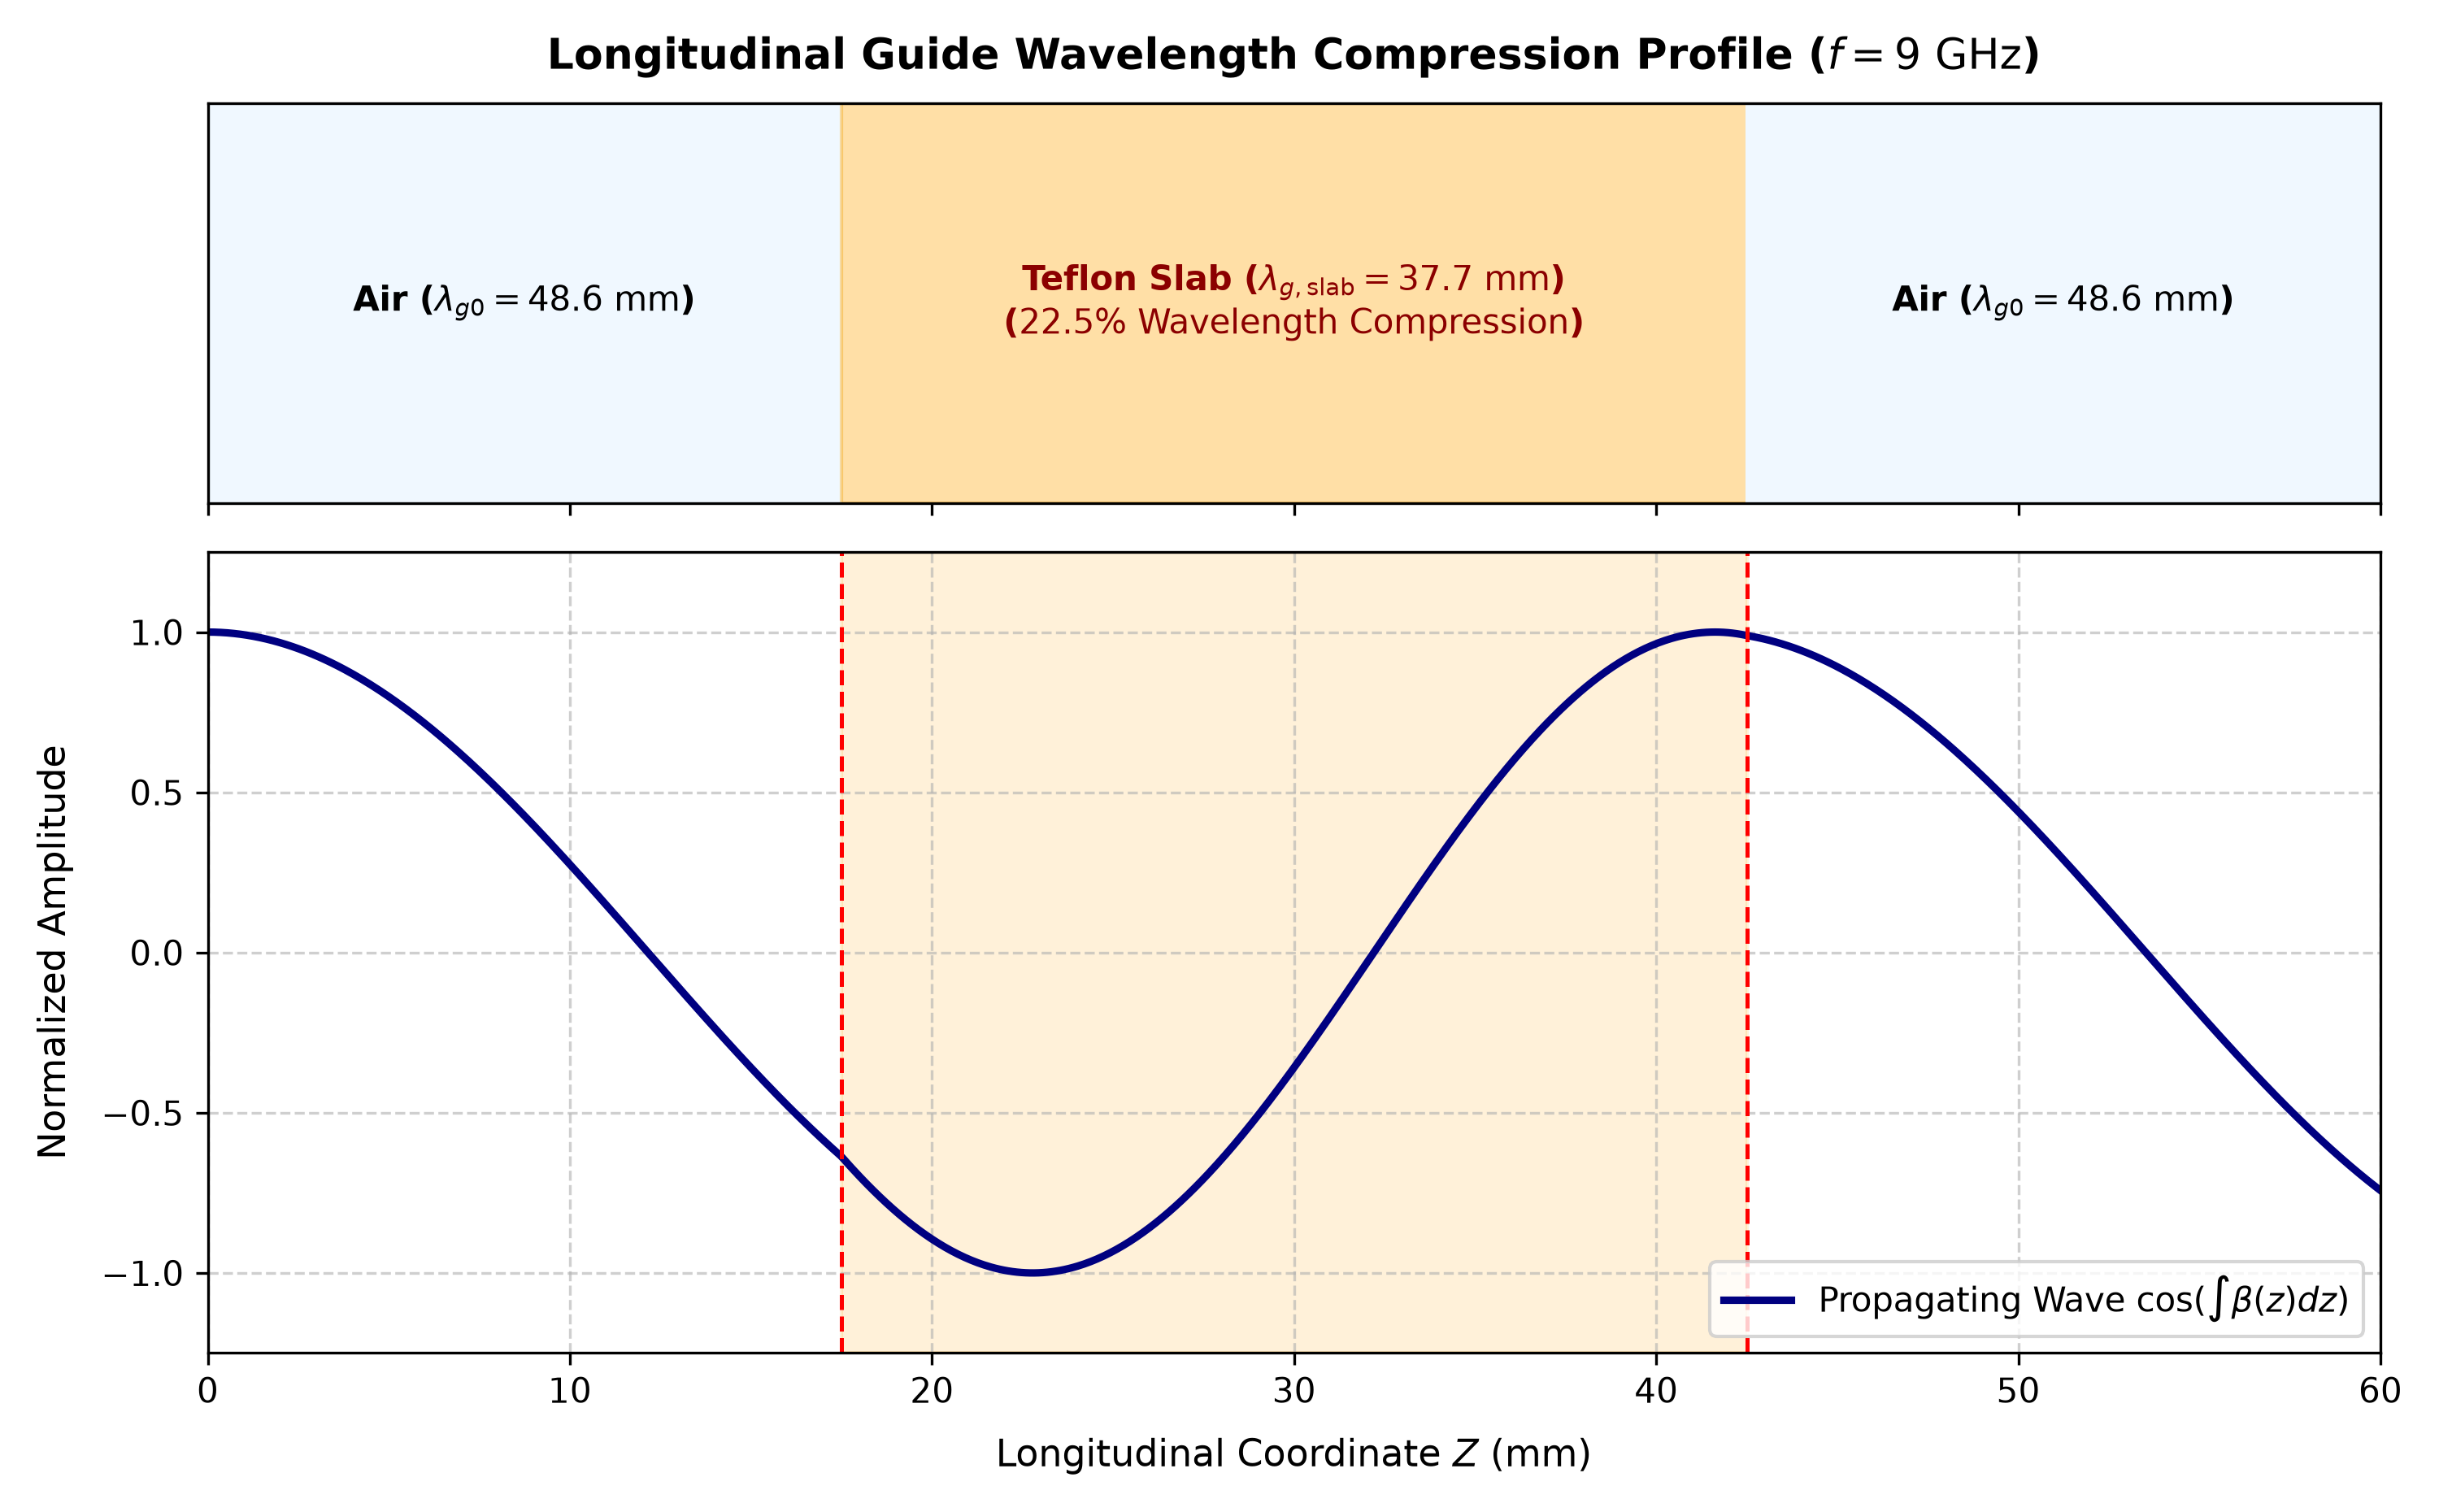
\includegraphics[width=0.92\textwidth]{img/longitudinal_wavelength_diagram.png}
    \caption{فشرده‌سازی طول موج هدایت‌شده ($\lambda_{g,\text{slab}} \approx 37.7\text{ mm}$) در ناحیه استقرار تیغه تفلون نسبت به بخش‌های تهی ($\lambda_{g0} = 48.63\text{ mm}$).}
    \label{fig:long_wave}
\end{figure}

\subsection{انتخاب جنس و ابعاد تیغه}
\begin{itemize}
    \item \textbf{جنس تیغه:} تفلون \lr{(PTFE / Teflon)} با گذردهی نسبی $\varepsilon_r = 2.1$ و ضریب اتلاف بسیار اندک $\tan\delta = 0.0002$. ضریب گذردهی ملایم تفلون باعث می‌شود پرش امپدانسی در لبه‌های تیغه کم باشد و عبور توان به حداکثر برسد.
    \item \textbf{ابعاد تیغه ($25 \times 10.16 \times 3\text{ mm}$):} طول $l_{\text{slab}} = 25.0\text{ mm}$، ارتفاع $b = 10.16\text{ mm}$ (پرکننده ارتفاع کامل) و ضخامت $t_{\text{slab}} = 3.0\text{ mm}$ انتخاب شده است.
    \item \textbf{موقعیت تیغه:} در راستای عرضی، در مرکز موج‌بر ($x=0$) قرار گرفته که ماکزیمم میدان الکتریکی مد $\text{TE}_{10}$ در آنجا متمرکز است تا بیشترین تغییر فاز با حداقل حجم دی‌الکتریک حاصل شود.
\end{itemize}

\begin{figure}[!htbp]
    \centering
    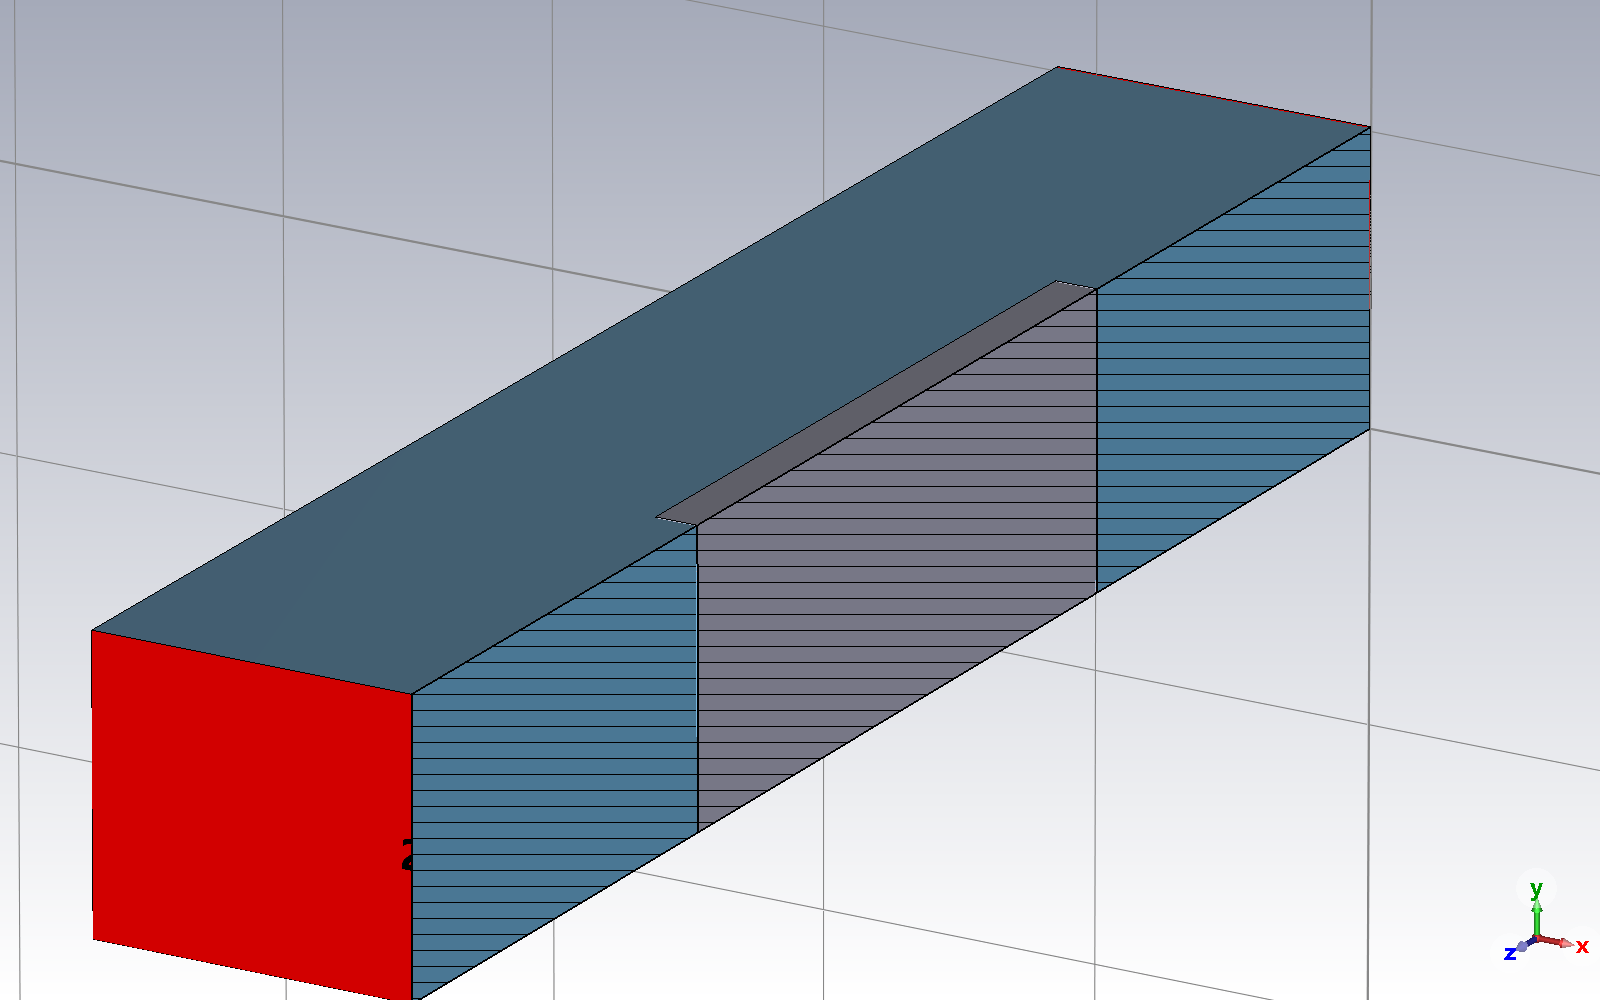
\includegraphics[width=0.75\textwidth]{img/waveguide_structure_3D.png}
    \caption{مدل هندسی سه‌بعدی موج‌بر بارگذاری‌شده با تیغه تفلون در نرم‌افزار \lr{CST Studio Suite}.}
    \label{fig:cad3d}
\end{figure}

\begin{table}[!htbp]
    \centering
    \caption{مشخصات هندسی و پارامتریک مدل در \lr{CST Studio Suite}}
    \vspace{0.2cm}
    \begin{tabular}{|c|c|c|c|}
        \hline
        \textbf{نام پارامتر} & \textbf{نماد در نرم‌افزار} & \textbf{مقدار} & \textbf{توضیحات هندسی} \\
        \hline
        عرض موج‌بر & \texttt{a} & $22.86\text{ mm}$ & بعد عریض موج‌بر استاندارد \lr{WR-90} \\
        \hline
        ارتفاع موج‌بر & \texttt{b} & $10.16\text{ mm}$ & بعد باریک موج‌بر \lr{WR-90} \\
        \hline
        طول کل موج‌بر & \texttt{length} & $60.0\text{ mm}$ & امتداد طولی در راستای محور Z \\
        \hline
        ضخامت تیغه & \texttt{t\_slab} & $3.0\text{ mm}$ & ضخامت دی‌الکتریک متقارن در مرکز \\
        \hline
        طول تیغه & \texttt{l\_slab} & $25.0\text{ mm}$ & امتداد طولی دی‌الکتریک در مرکز موج‌بر \\
        \hline
        گذردهی نسبی & \texttt{eps\_r} & $2.1$ & تفلون با تلفات ناچیز ($\tan\delta = 2 \times 10^{-4}$) \\
        \hline
    \end{tabular}
    \label{tab:params}
\end{table}

\section{شبیه‌سازی در \lr{CST Studio Suite} و تحلیل پارامترهای پراکندگی}

مدل‌سازی به صورت تمام‌پارامتریک در نرم‌افزار \lr{\lr{CST Studio Suite} 2026} انجام گرفت. دیواره‌های بیرونی از جنس هادی ایده‌آل \lr{(PEC)} و دو پورت موج‌بری \lr{(Waveguide Ports)} در مقاطع ورودی ($Z=0$) و خروجی ($Z=60\text{ mm}$) قرار داده شدند. حل‌کننده حوزه فرکانس \lr{(Frequency Domain Solver)} مبتنی بر شبکه تتراهدرال جهت حل دقیق میدان‌ها استفاده شد.

\subsection{نمودار اندازه پارامترهای پراکندگی (\texorpdfstring{$|S_{11}|$ و $|S_{21}|$}{|S11| و |S21|})}
پاسخ فرکانسی اندازه پارامترهای $S_{11}$ و $S_{21}$ در بازه فرکانسی $7.0\text{ GHz}$ تا $12.0\text{ GHz}$ در \autoref{fig:s_mag} ترسیم شده است.

\begin{figure}[!htbp]
    \centering
    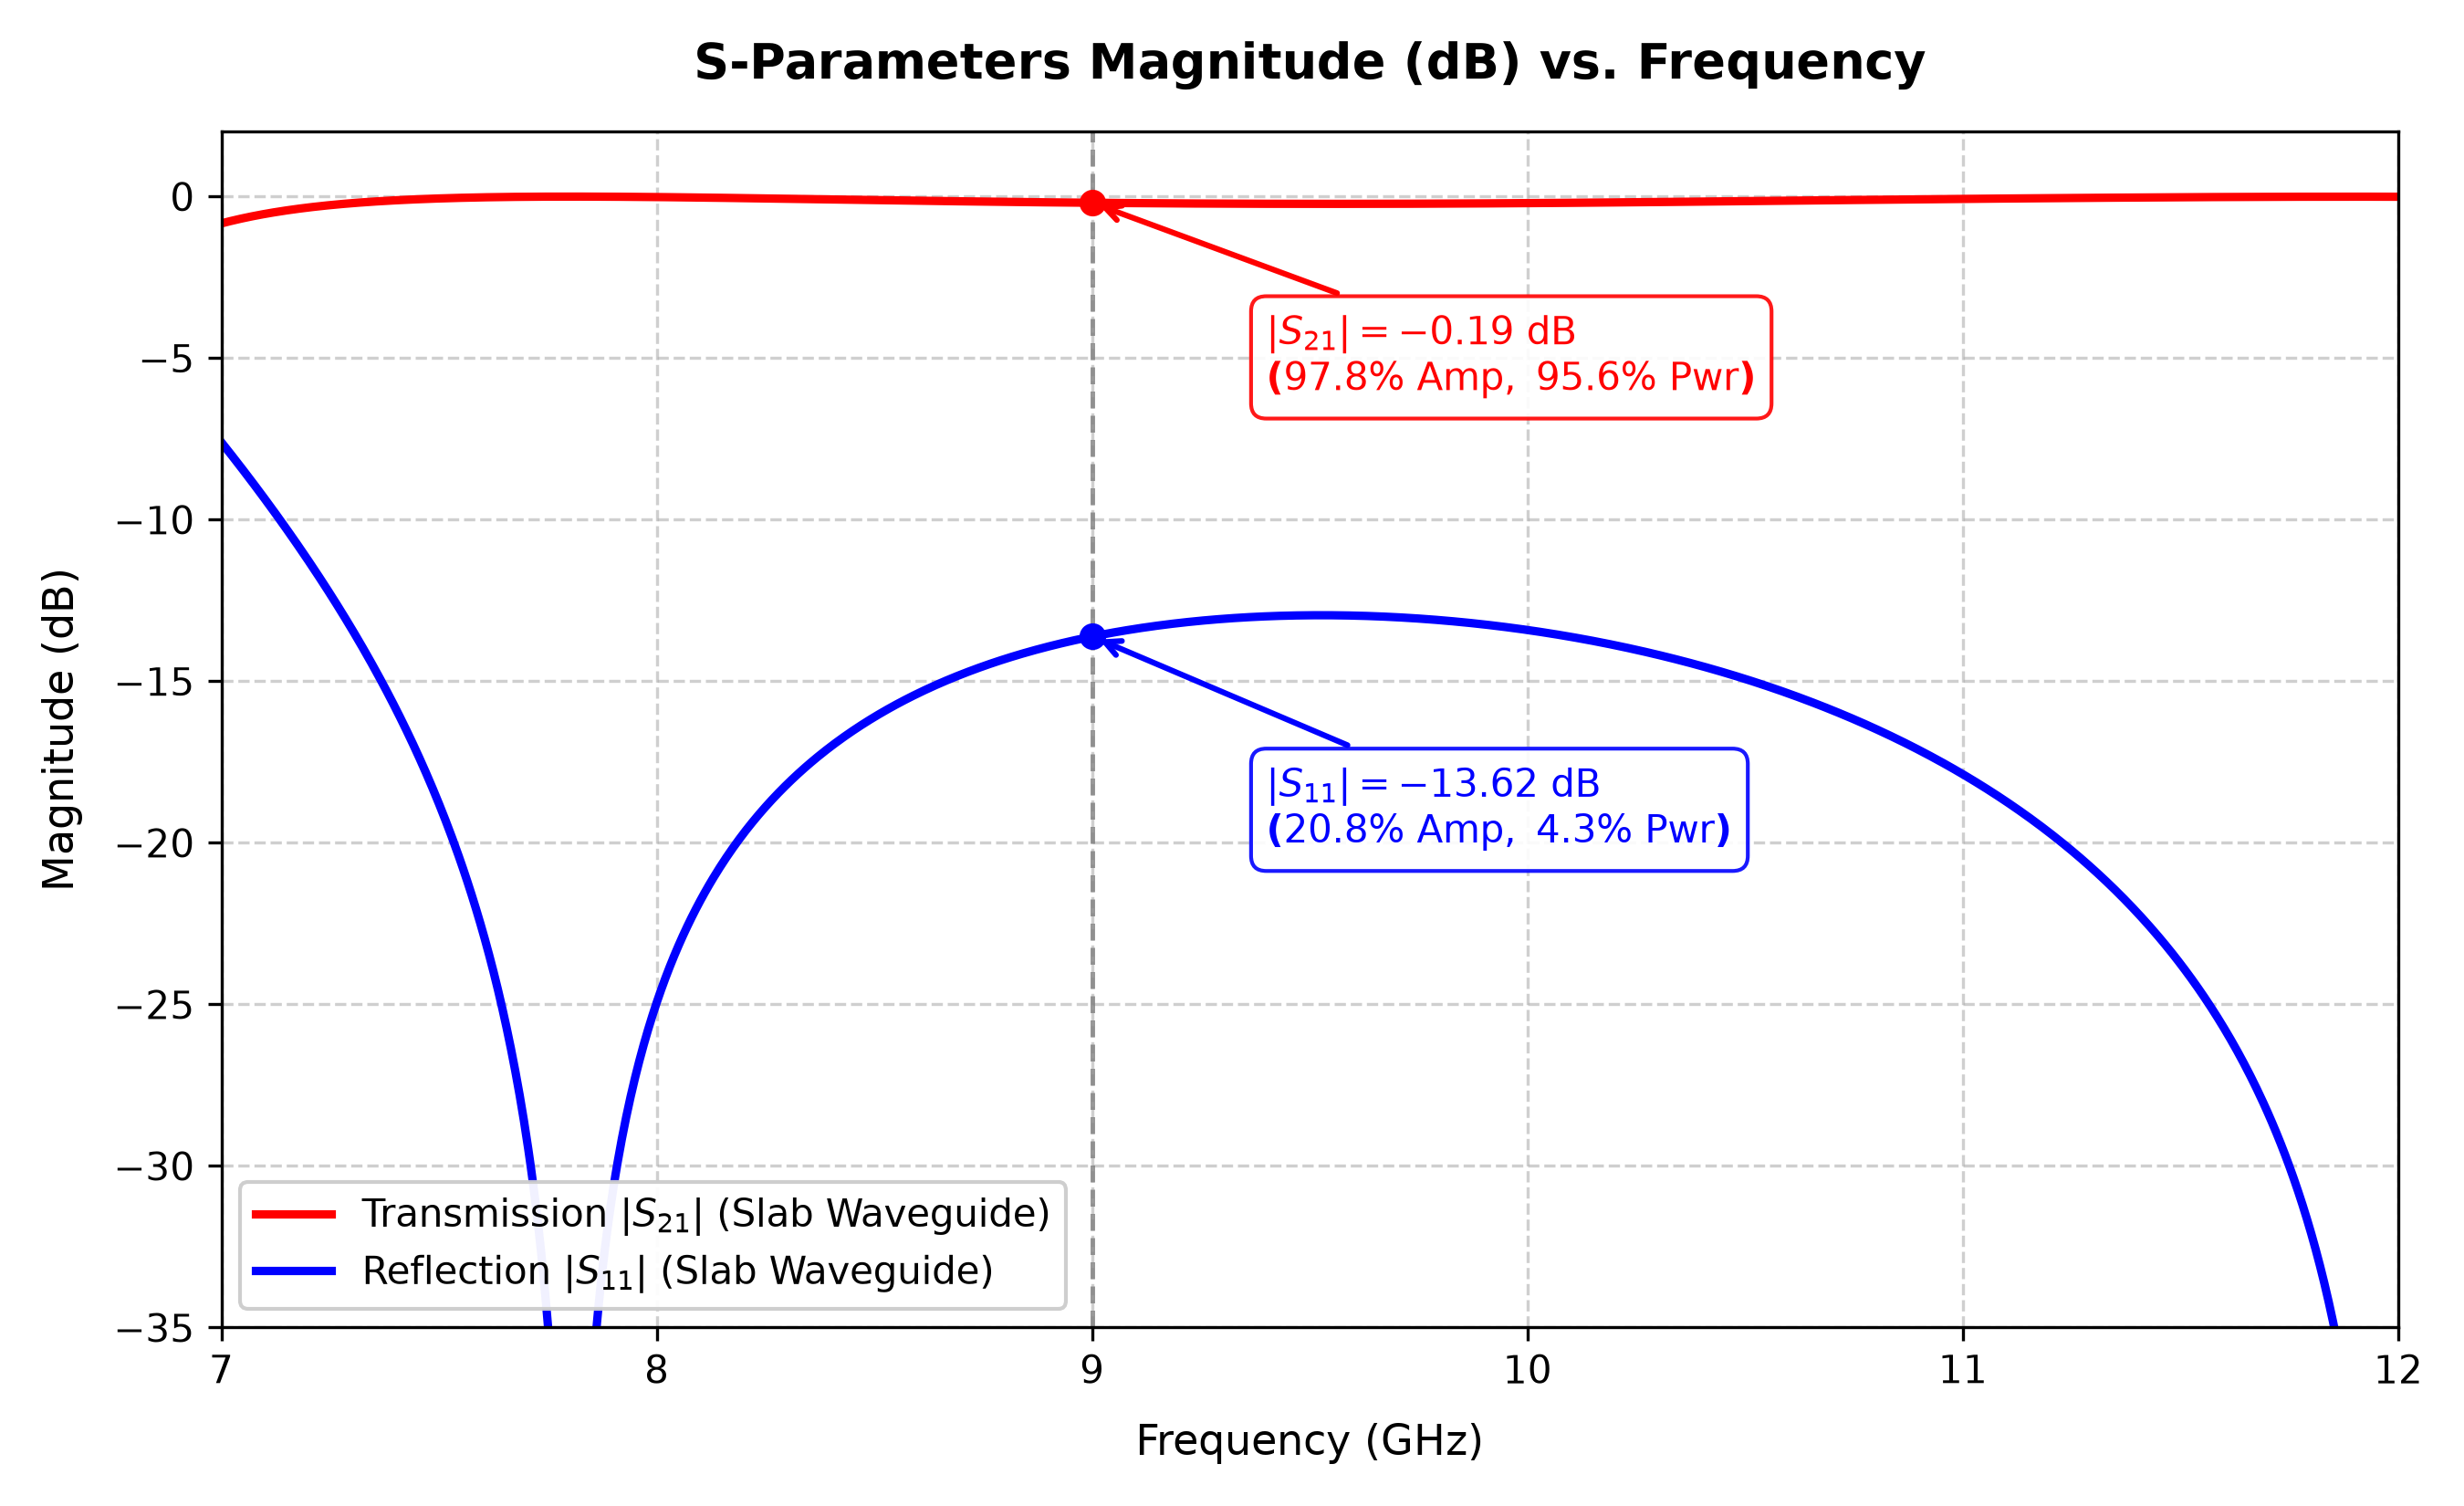
\includegraphics[width=0.88\textwidth]{img/s_parameters_magnitude_v2.png}
    \caption{پاسخ فرکانسی اندازه پارامترهای پراکندگی $|S_{11}|$ و $|S_{21}|$ بر حسب دسی‌بل در بازه ۷ تا ۱۲ گیگاهرتز.}
    \label{fig:s_mag}
\end{figure}

در فرکانس مرکزی $9.0\text{ GHz}$:
\begin{itemize}
    \item \textbf{ضریب انتقال:} $|S_{21}| = -0.194\text{ dB}$ است. این مقدار بیانگر انتقال **$97.8\%$ از دامنه ولتاژ** ($10^{-0.194/20} = 0.9779$) و **$95.6\%$ از توان ورودی** ($|S_{21}|^2 = 10^{-0.194/10} = 0.9563$) است.
    \item \textbf{ضریب بازتاب:} $|S_{11}| = -13.62\text{ dB}$ است که معادل بازتاب دامنه $20.8\%$ و بازتاب توان $4.3\%$ می‌باشد ($0.9563 + 0.0433 \approx 1.0$).
\end{itemize}

\textbf{تحلیل فیزیکی بازتاب ناچیز:}
بازتاب ساختار ناشی از دو ناپیوستگی پله‌ای ناگهانی در مرز ورودی تیغه ($Z=17.5\text{ mm}$) و مرز خروجی تیغه ($Z=42.5\text{ mm}$) است. علت اینکه بازتاب در سطح پایینی (زیر $4.3\%$ توان) باقی مانده، کنتراست گذردهی ملایم تفلون ($\varepsilon_r = 2.1$) و تقابل فاز موج‌های بازتابی از دو لبه است، نه تغییر تدریجی امپدانس.

\subsection{نمودار فاز پارامترهای پراکندگی (\texorpdfstring{$\angle S_{11}$ و $\angle S_{21}$}{Phase S11 and S21})}
برای درک پیوسته از فاز انتقال، رفتار فاز بازشده \lr{(Unwrapped Phase)} پارامترهای پراکندگی در \autoref{fig:s_phase_unwrapped} ارائه شده است.

\begin{figure}[!htbp]
    \centering
    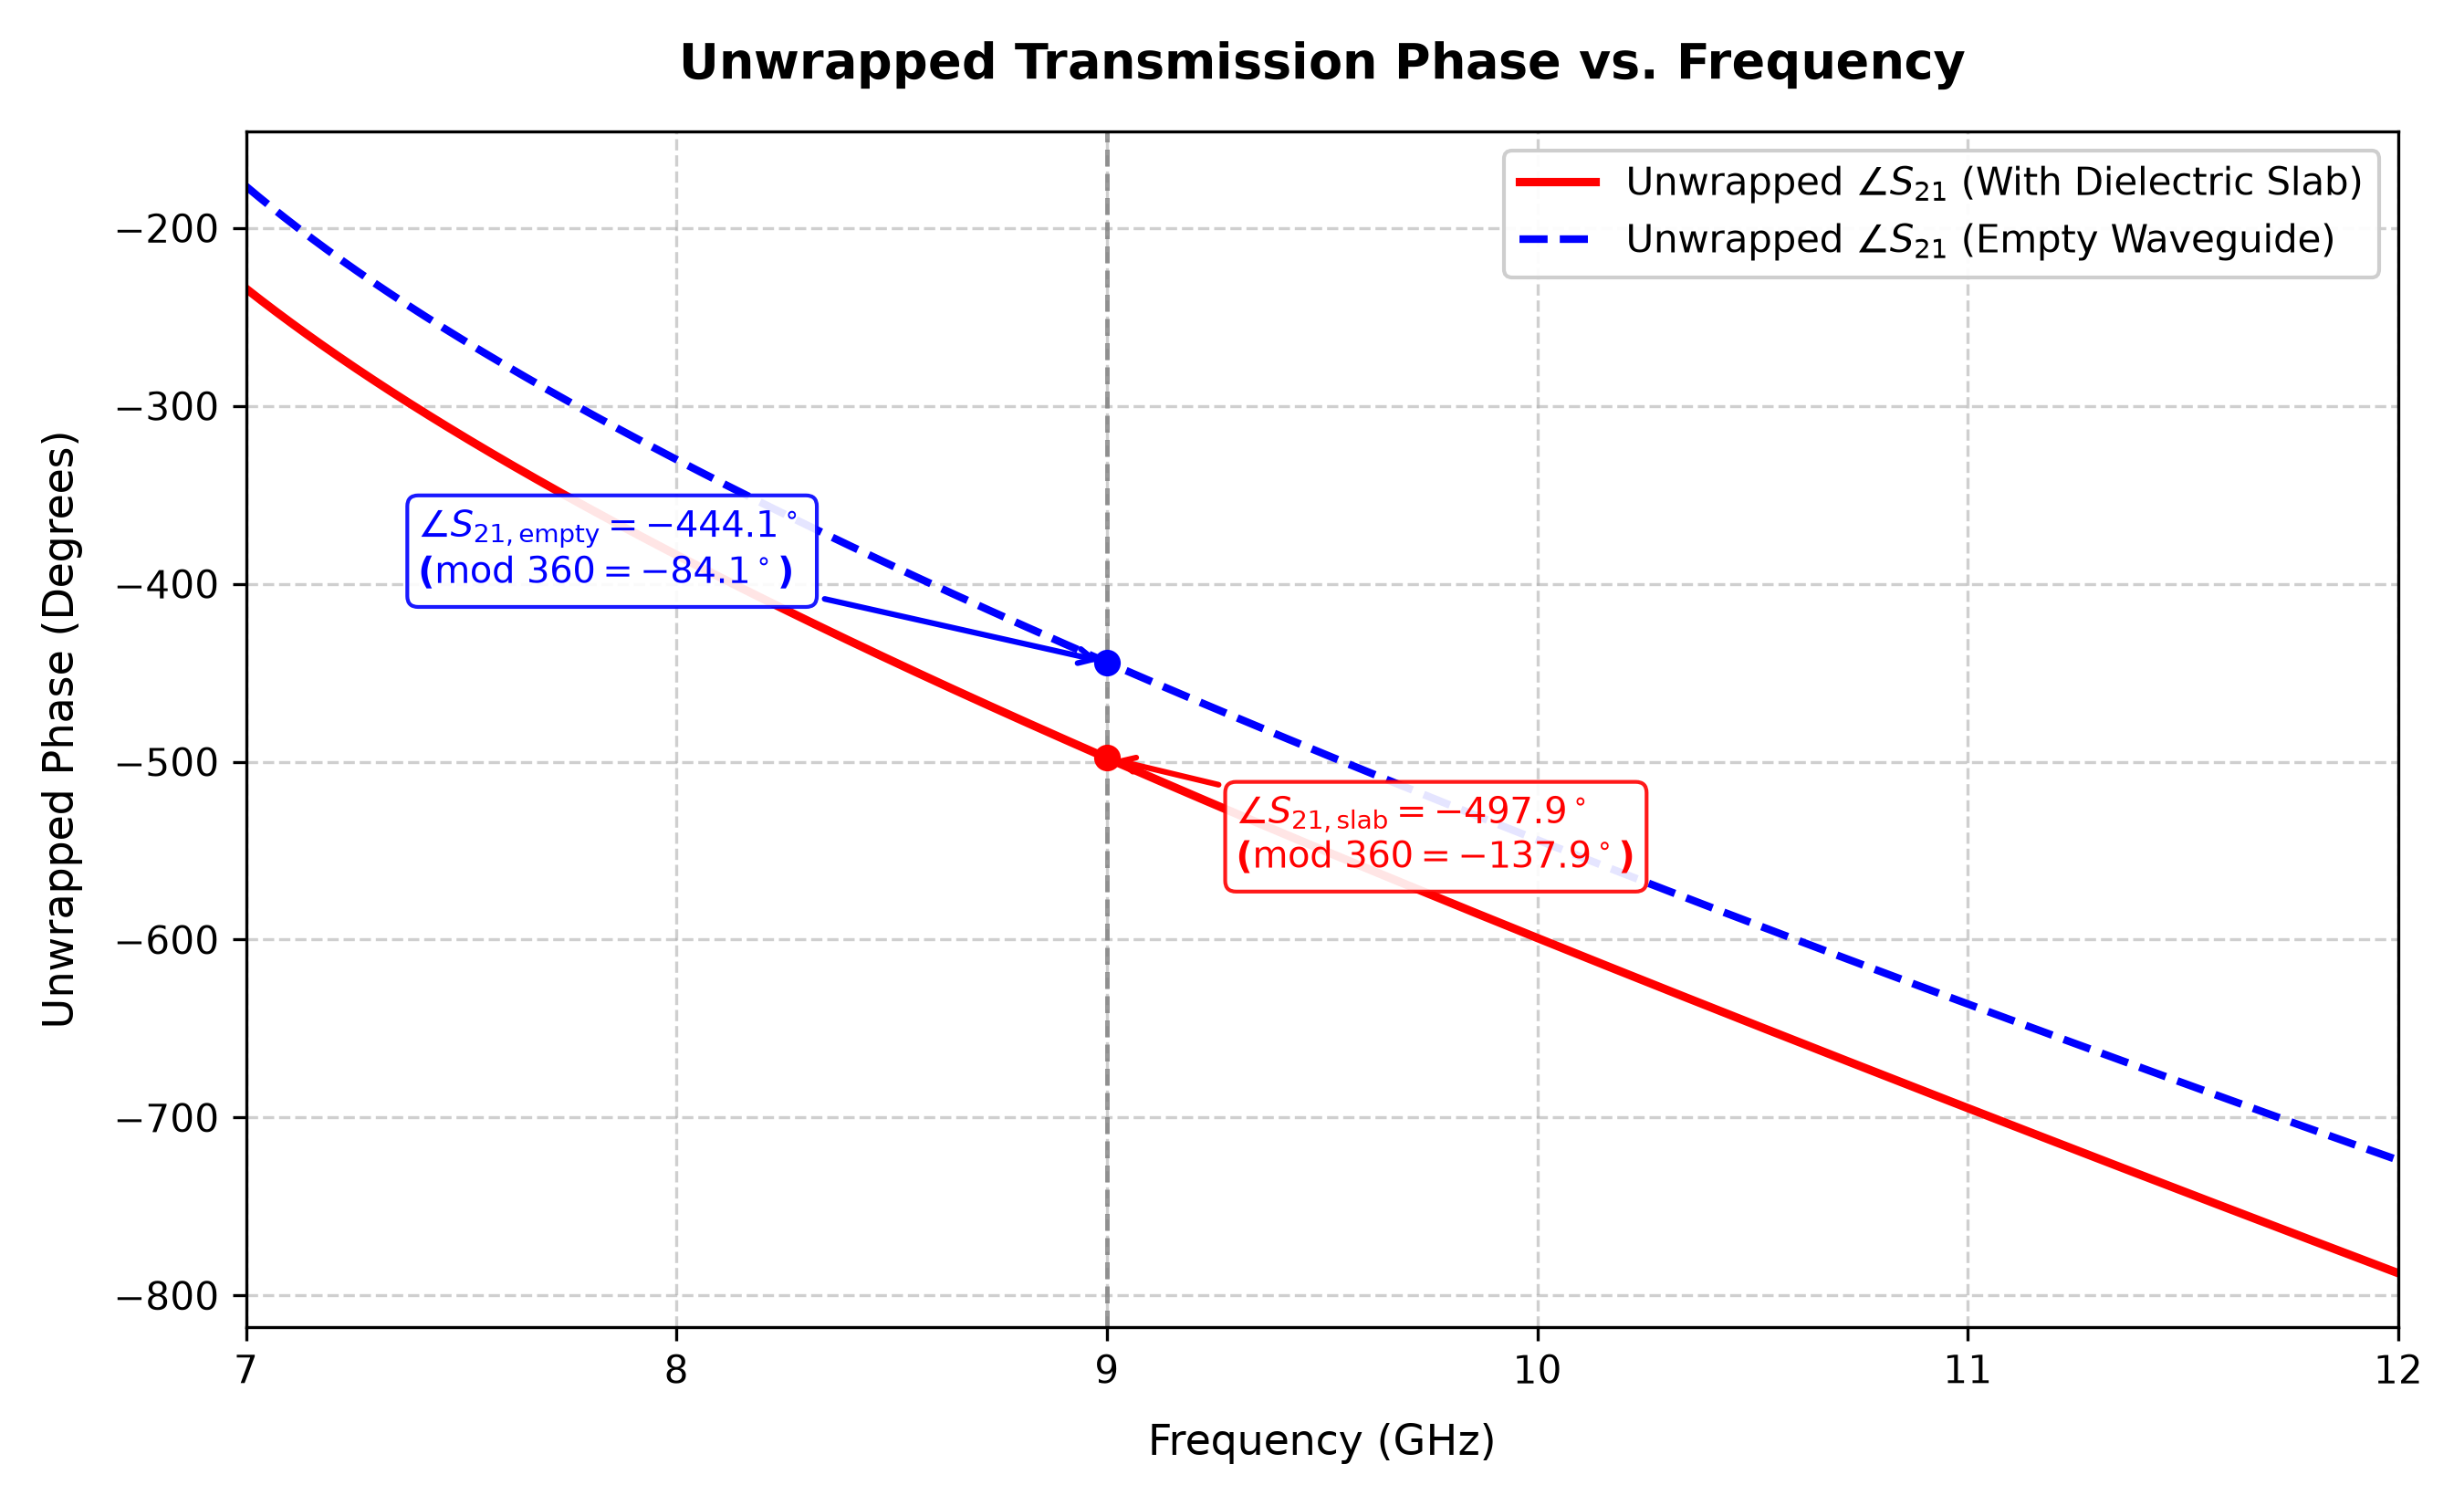
\includegraphics[width=0.88\textwidth]{img/s_parameters_phase_unwrapped.png}
    \caption{رفتار فاز بازشده (Unwrapped) پارامترهای انتقال در دو حالت با تیغه و بدون تیغه.}
    \label{fig:s_phase_unwrapped}
\end{figure}

در فرکانس $9\text{ GHz}$:
\begin{itemize}
    \item فاز انتقال واقعی بدون برش موج‌بر حاوی تیغه برابر $\angle S_{21,\text{slab}} = -497.92^\circ$ است که در محدوده بازه اصلی نرم‌افزار معادل $-137.92^\circ$ گزارش می‌شود ($-497.92^\circ + 360^\circ = -137.92^\circ$).
    \item فاز انتقال واقعی موج‌بر خالی برابر $\angle S_{21,\text{empty}} = -444.13^\circ$ (معادل $-84.13^\circ$) است.
    \item اختلاف این دو فاز بازشده مستقیماً شیفت فاز تفاضلی $53.79^\circ$ را آشکار می‌سازد.
\end{itemize}

\section{مقایسه عملکرد: حالت با تیغه دی‌الکتریک و موجبر خالی}
برای اعتبارسنجی مستقل، ساختار یک‌بار با تیغه تفلون ($\varepsilon_r = 2.1$) و بار دیگر با جایگزینی هوا ($\varepsilon_r = 1.0$) تحت شرایط شبیه‌سازی یکسان اجرا شد. نمودار شیفت فاز تفاضلی $\Delta\phi(f)$ بر حسب فرکانس در \autoref{fig:delta_phi} رسم شده است.

\begin{figure}[!htbp]
    \centering
    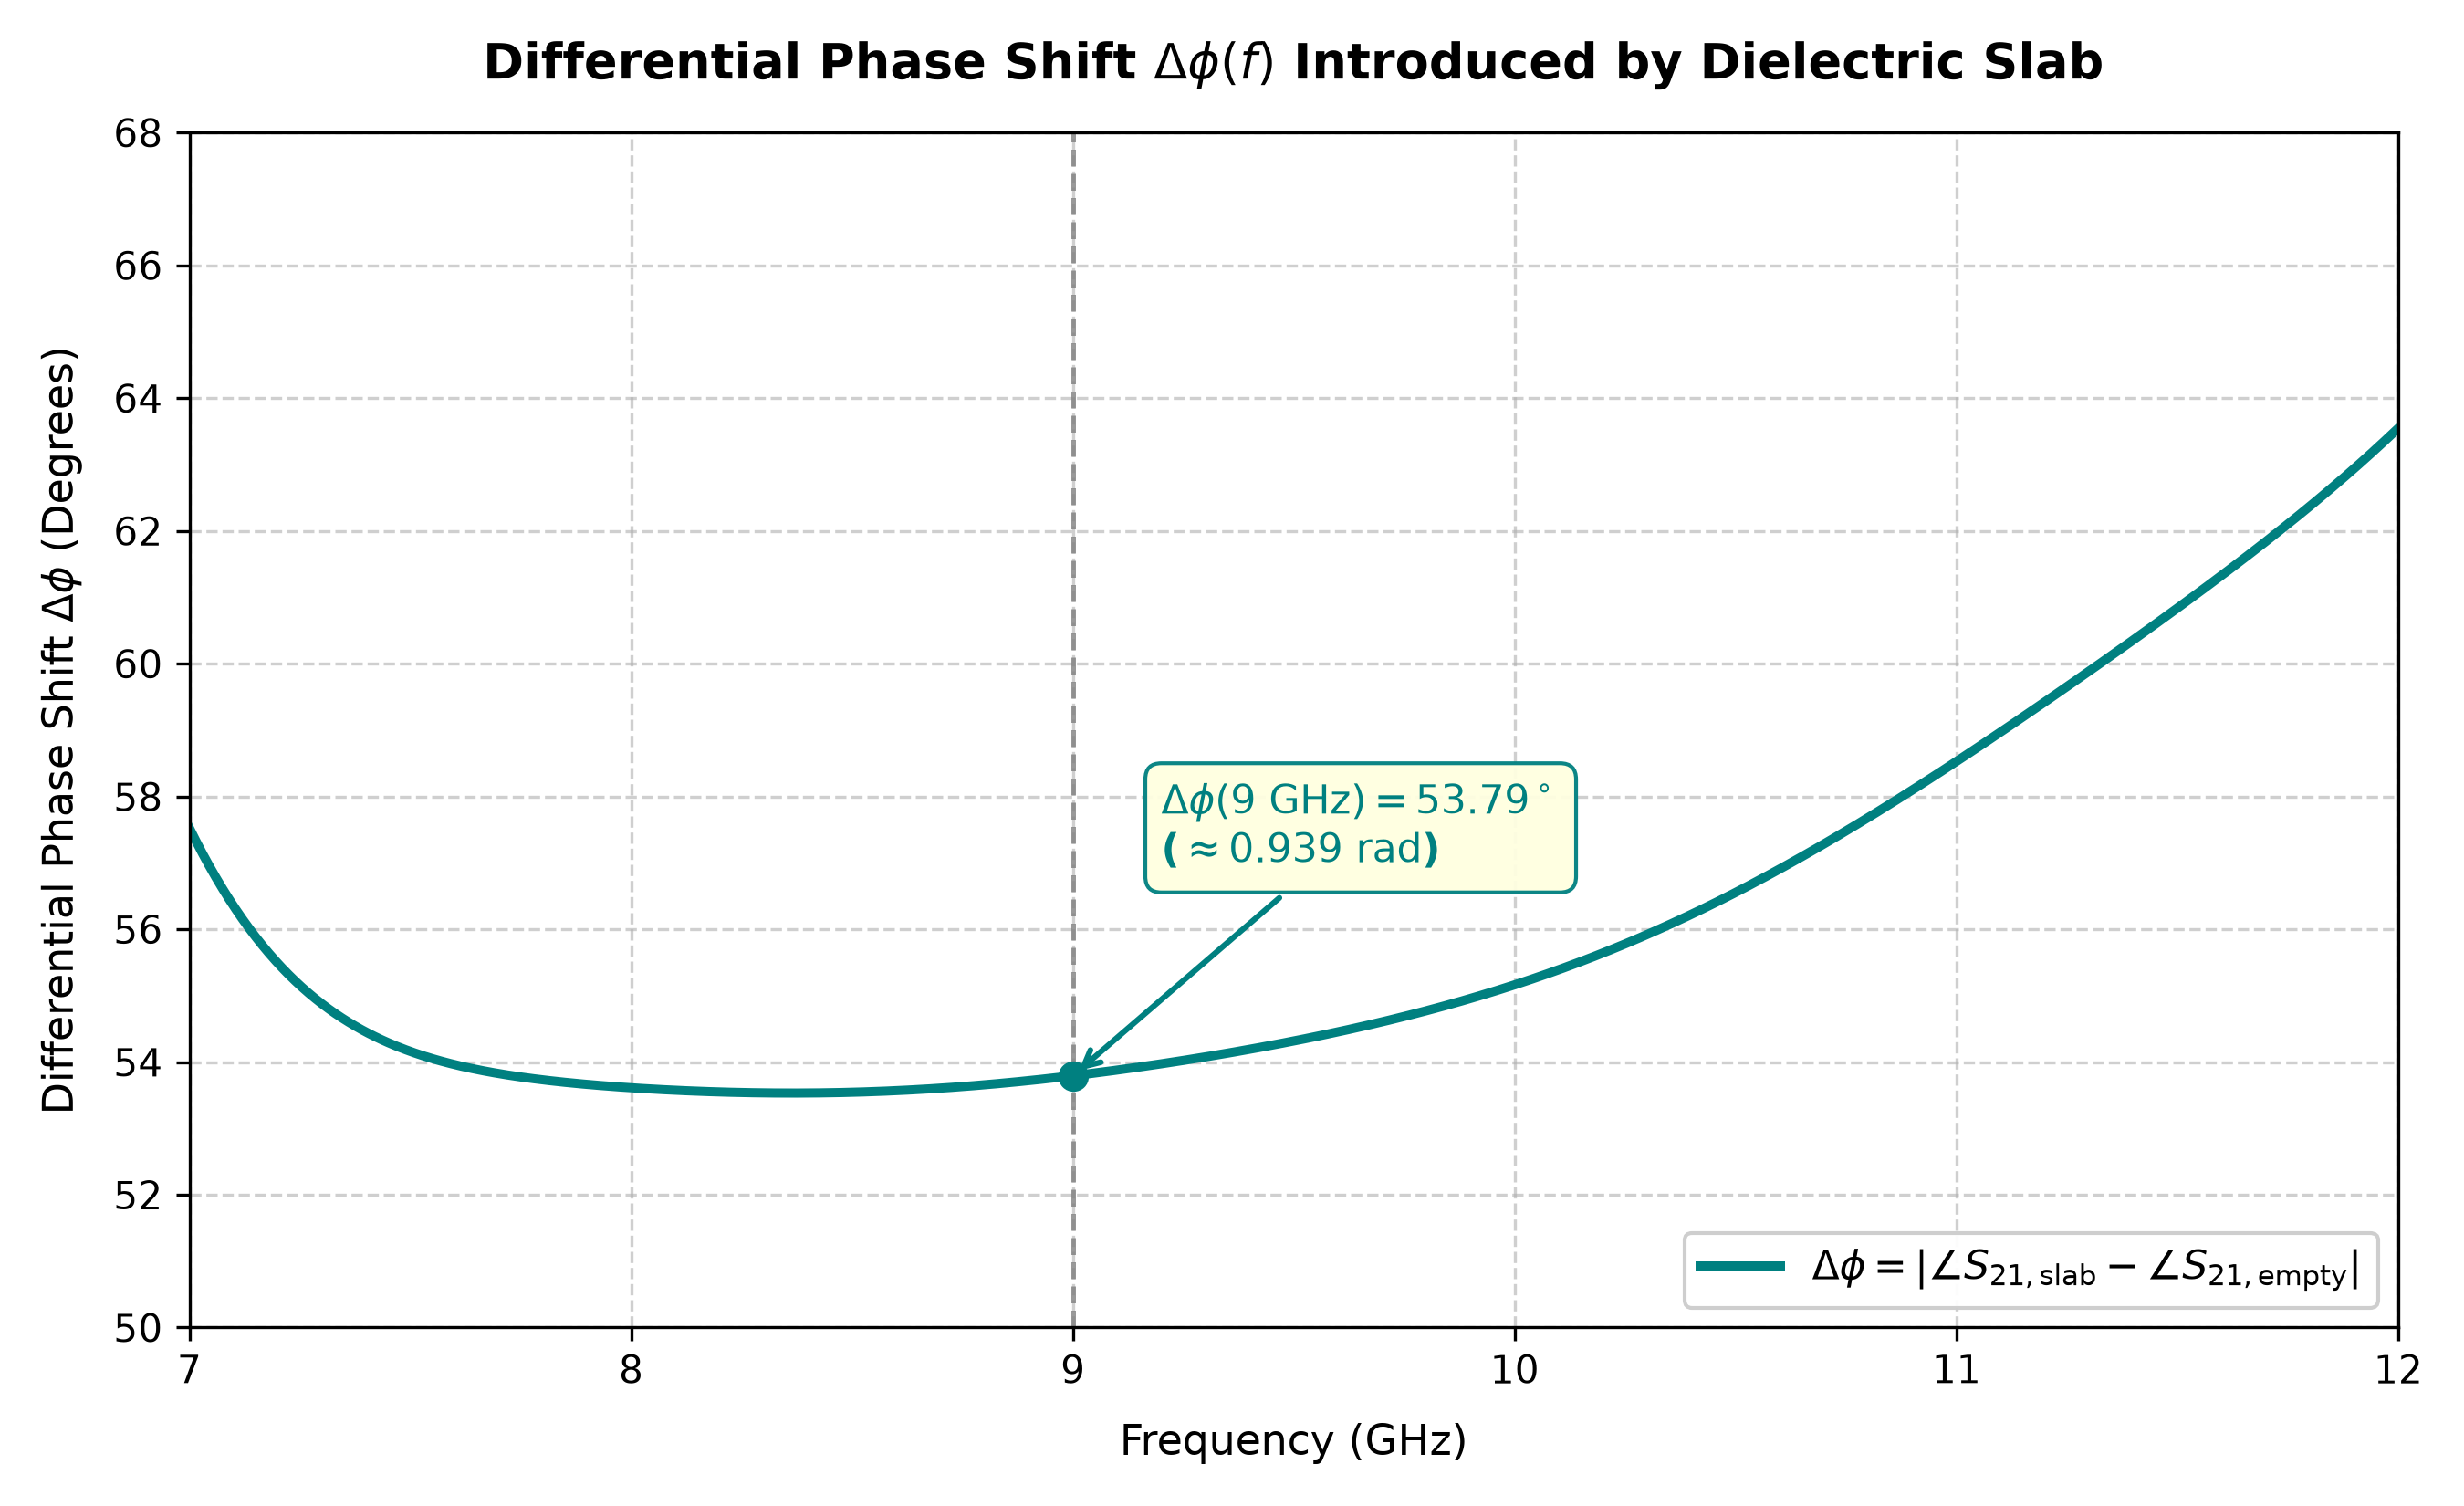
\includegraphics[width=0.88\textwidth]{img/delta_phi_vs_freq.png}
    \caption{نمودار پاسخ فرکانسی شیفت فاز تفاضلی $\Delta\phi(f) = |\angle S_{21,\text{slab}} - \angle S_{21,\text{empty}}|$ در بازه ۷ تا ۱۲ گیگاهرتز.}
    \label{fig:delta_phi}
\end{figure}

\begin{table}[!htbp]
    \centering
    \caption{مقایسه عددی مشخصات موج‌بر در فرکانس $9.0\text{ GHz}$}
    \vspace{0.2cm}
    
    \resizebox{\textwidth}{!}{%
    \begin{tabular}{|c|c|c|c|}
        \hline
        \textbf{مشخصه} & \textbf{موج‌بر خالی (بدون تیغه)} & \textbf{موج‌بر با تیغه تفلون} & \textbf{اثر تیغه دی‌الکتریک} \\
        \hline
        ضریب بازتاب $|S_{11}|$ & $-87.74\text{ dB}$ & $-13.62\text{ dB}$ & بازتاب اندک ناشی از دو لبه پله‌ای \\
        \hline
        ضریب انتقال $|S_{21}|$ & $-0.002\text{ dB}$ & $-0.194\text{ dB}$ & افت توان بسیار ناچیز ($4.4\%$) \\
        \hline
        فاز انتقال $\angle S_{21}$ & $-84.13^\circ$ (واقعی: $-444.1^\circ$) & $-137.92^\circ$ (واقعی: $-497.9^\circ$) & تاخیر زمانی موج \\
        \hline
        \textbf{شیفت فاز تفاضلی ($\Delta\phi$)} & $0^\circ$ & \textbf{$53.79^\circ$} & \textbf{شیفتر فاز با بازتاب اندک} \\
        \hline
        طول موج هدایت‌شده & $\lambda_{g0} = 48.63\text{ mm}$ & $\lambda_{g,\text{slab}} \approx 37.7\text{ mm}$ & فشرده‌سازی مکانی طول موج \\
        \hline
    \end{tabular}%
    }
    \label{tab:compare}
\end{table}

\section{بررسی همگرایی مش (Mesh Convergence Analysis)}
برای اطمینان از استقلال نتایج عددی از شبکه المان‌ها، شبیه‌سازی با دو تراکم مش مش‌بندی تتراهدرال اولیه (\lr{Coarse}) و مش متراکم بهینه‌سازی‌شده (\lr{Fine}) اجرا گردید.

\begin{table}[!htbp]
    \centering
    \caption{بررسی همگرایی مش در فرکانس $9.0\text{ GHz}$}
    \vspace{0.2cm}
    \begin{tabular}{|c|c|c|c|c|}
        \hline
        \textbf{سطح مش} & \textbf{تعداد المان‌های تتراهدرال} & $|S_{11}|\text{ (dB)}$ & $|S_{21}|\text{ (dB)}$ & \textbf{درجه آزادی} \\
        \hline
        مش اولیه (\lr{Coarse}) & $1,865$ & $-13.617$ & $-0.194$ & $10,840$ \\
        \hline
        مش متراکم (\lr{Fine}) & $3,330$ & $-13.610$ & $-0.195$ & $19,432$ \\
        \hline
        \textbf{تغییرات ($\Delta$)} & $+78.5\%$ & \textbf{$0.007\text{ dB}$} & \textbf{$0.001\text{ dB}$} & \textbf{همگرایی کامل} \\
        \hline
    \end{tabular}
    \label{tab:mesh}
\end{table}
تغییرات کمتر از $0.007\text{ dB}$ در ضریب بازتاب و کمتر از $0.001\text{ dB}$ در ضریب عبور، صحت همگرایی کامل حل عددی را به اثبات می‌رساند.

\section{تحلیل توزیع میدان‌های الکترومغناطیسی: مقایسه برداری و کانتوری}

توزیع میدان‌های الکتریکی ($\vec{E}$) و مغناطیسی ($\vec{H}$) در فرکانس $9.0\text{ GHz}$ در سه مقطع بررسی شده است:
\begin{enumerate}
    \item \textbf{مقطع عرضی \lr{(Transverse XY Cut)}}: در مرکز موج‌بر $Z = 30\text{ mm}$ عمود بر امتداد انتشار.
    \item \textbf{صفحه طولی افقی \lr{(Horizontal Longitudinal XZ Cut)}}: در نیمه ارتفاع موج‌بر $Y = b/2 = 5.08\text{ mm}$.
    \item \textbf{صفحه طولی عمودی \lr{(Vertical Longitudinal YZ Cut)}}: در صفحه تقارن $X = 0\text{ mm}$.
\end{enumerate}

\subsection{مقایسه مفاهیم نمایش برداری و کانتوری پیوسته}
\begin{itemize}
    \item \textbf{نمایش برداری (Vector Plot):} با استفاده از بردارها، جهت لحظه‌ای میدان، پلاریزاسیون خطی و شرط مرزی صفر بودن میدان مماس بر هادی ($E_{\text{tan}} = 0$) را نمایش می‌دهد.
    \item \textbf{نمایش کانتوری و سطحی (Smooth Shaded Contour Plot):} این نمایش گرادیان پیوسته شدت میدان را به صورت نقشه‌ای رنگی و بدون خطوط تراز مزاحم نشان می‌دهد. شایان توجه است که در الکترودینامیک با میدان‌های متغیر با زمان ($\nabla \times \vec{E} \ne 0$)، خطوط تراز بیانگر ترازهای شدت میدان هستند و نباید با خطوط هم‌پتانسیل الکترواستاتیک اشتباه گرفته شوند. مزیت این نمایش در آشکارسازی نقاط تمرکز انرژی در تیغه دی‌الکتریک بدون شلوغی بصری فلش‌ها است. مقیاس رنگ برای تمام شکل‌های میدان الکتریکی در بازه $0$ تا $2700\text{ V/m}$ و برای میدان‌های مغناطیسی در بازه $0$ تا $5.2\text{ A/m}$ ثابت نگه داشته شده است.
\end{itemize}

\subsection{مقطع عرضی ($XY$) در $Z = 30\text{ mm}$}
در مقطع عرضی، فلش‌های میدان الکتریکی مد $\text{TE}_{10}$ کاملاً عمودی در امتداد محور $y$ هستند. میدان روی دیواره‌های جانبی صفر شده و در مرکز موج‌بر به بیشینه می‌رسد. در نمایش کانتوری، تمرکز رنگ گرم درون تیغه تفلون، چگالی انرژی بالاتر به دلیل گذردهی دی‌الکتریک را اثبات می‌کند.

\begin{figure}[!htbp]
    \centering
    \begin{subfigure}[b]{0.48\textwidth}
        \centering
        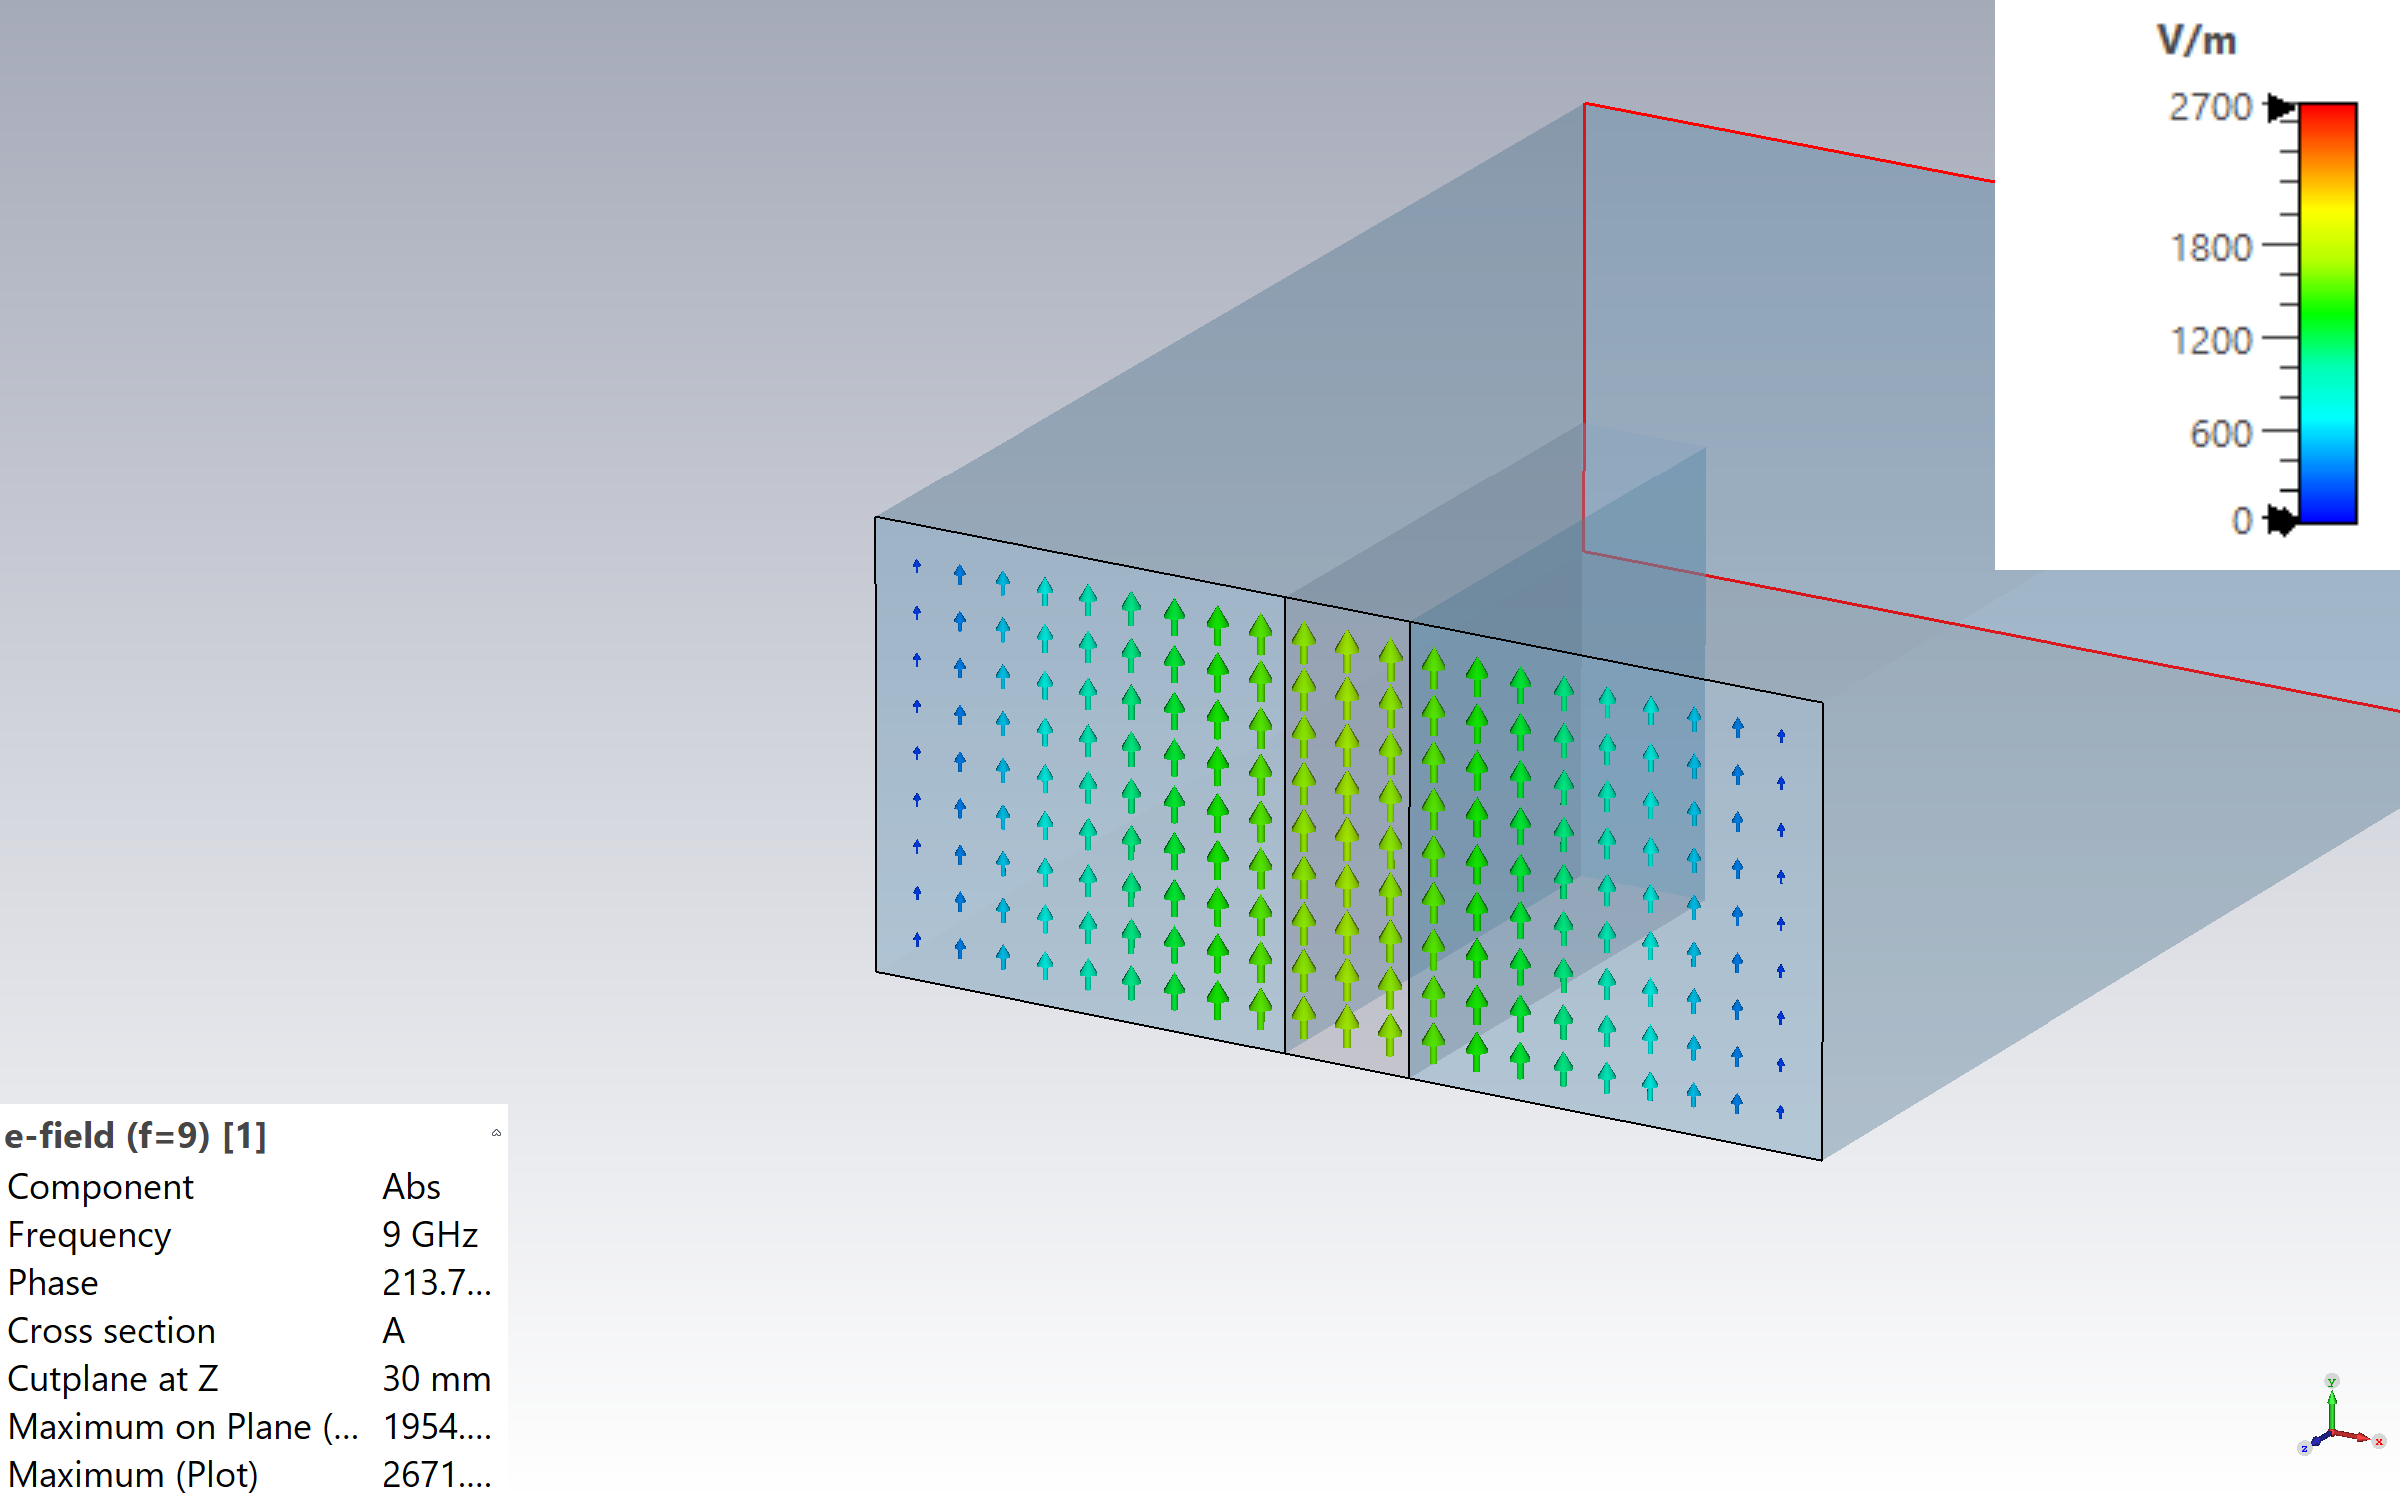
\includegraphics[width=\textwidth]{img/efield_v2_vector_XY.png}
        \caption{میدان الکتریکی --- نمای برداری}
    \end{subfigure}
    \hfill
    \begin{subfigure}[b]{0.48\textwidth}
        \centering
        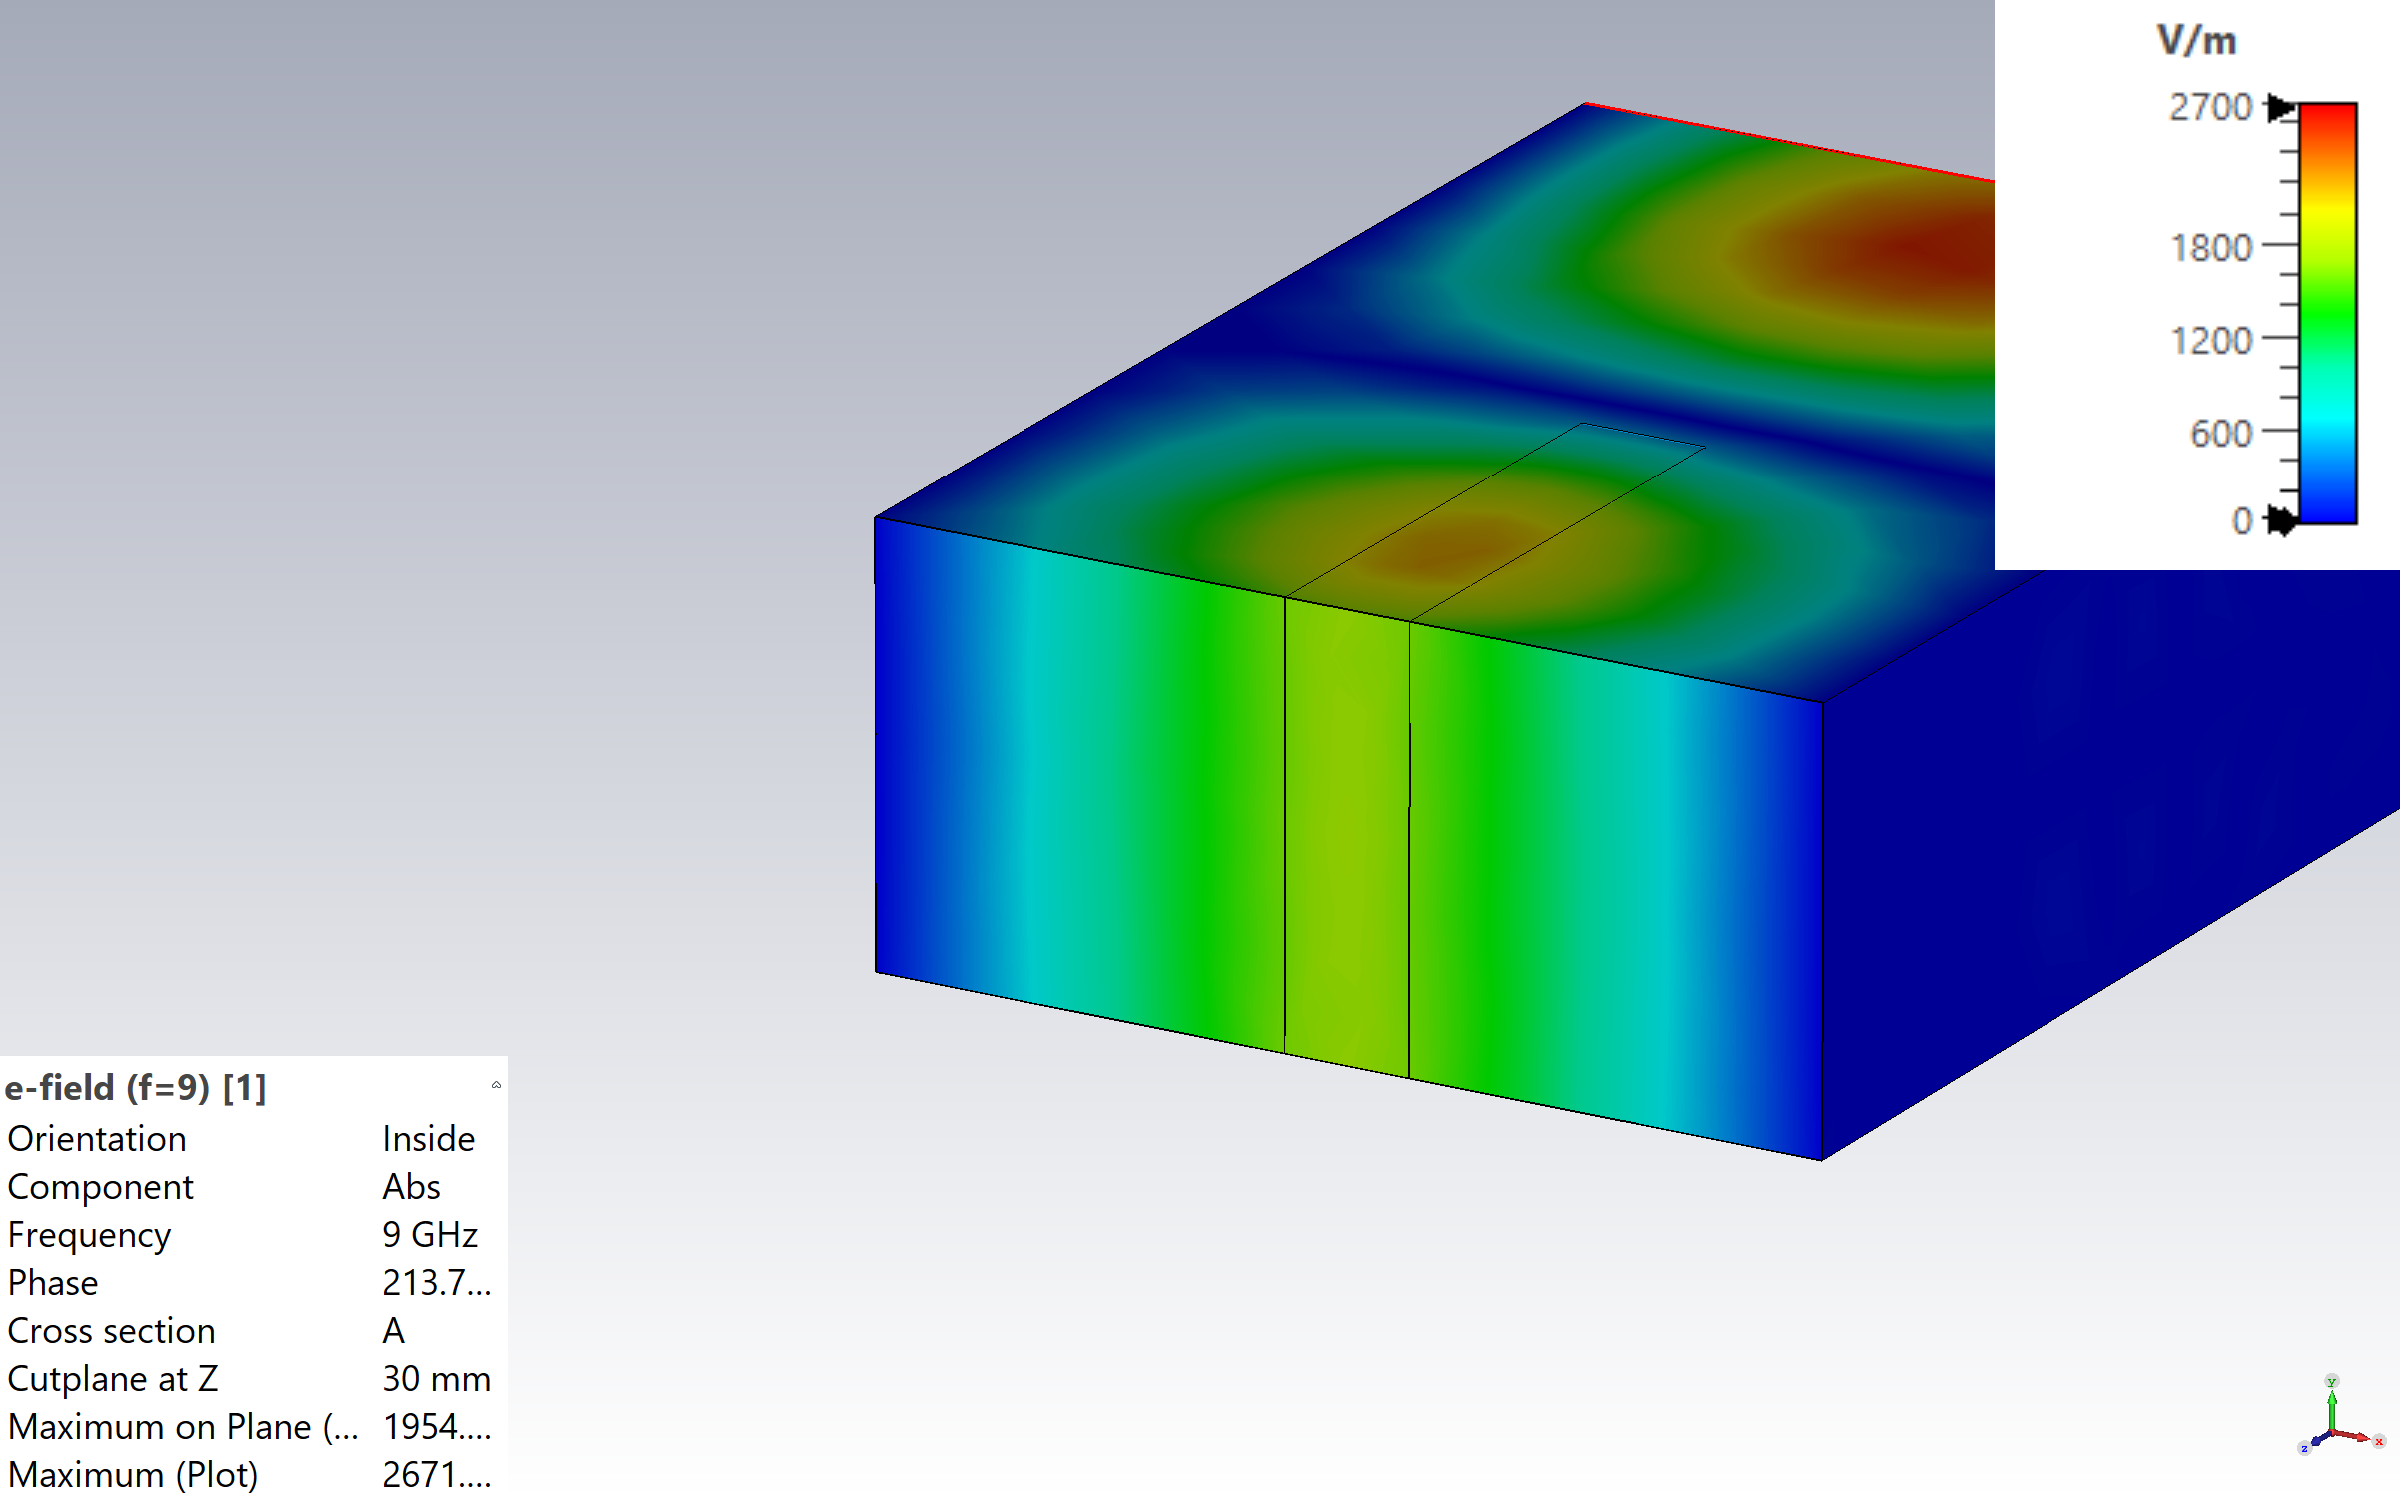
\includegraphics[width=\textwidth]{img/efield_v2_contour_XY.png}
        \caption{میدان الکتریکی --- نمای کانتوری پیوسته}
    \end{subfigure}
    \caption{توزیع میدان الکتریکی در مقطع عرضی ($XY$) در $Z=30\text{ mm}$ (مقیاس یکنواخت: ۰ تا ۲۷۰۰ ولت بر متر).}
    \label{fig:e_xy}
\end{figure}

\begin{figure}[!htbp]
    \centering
    \begin{subfigure}[b]{0.48\textwidth}
        \centering
        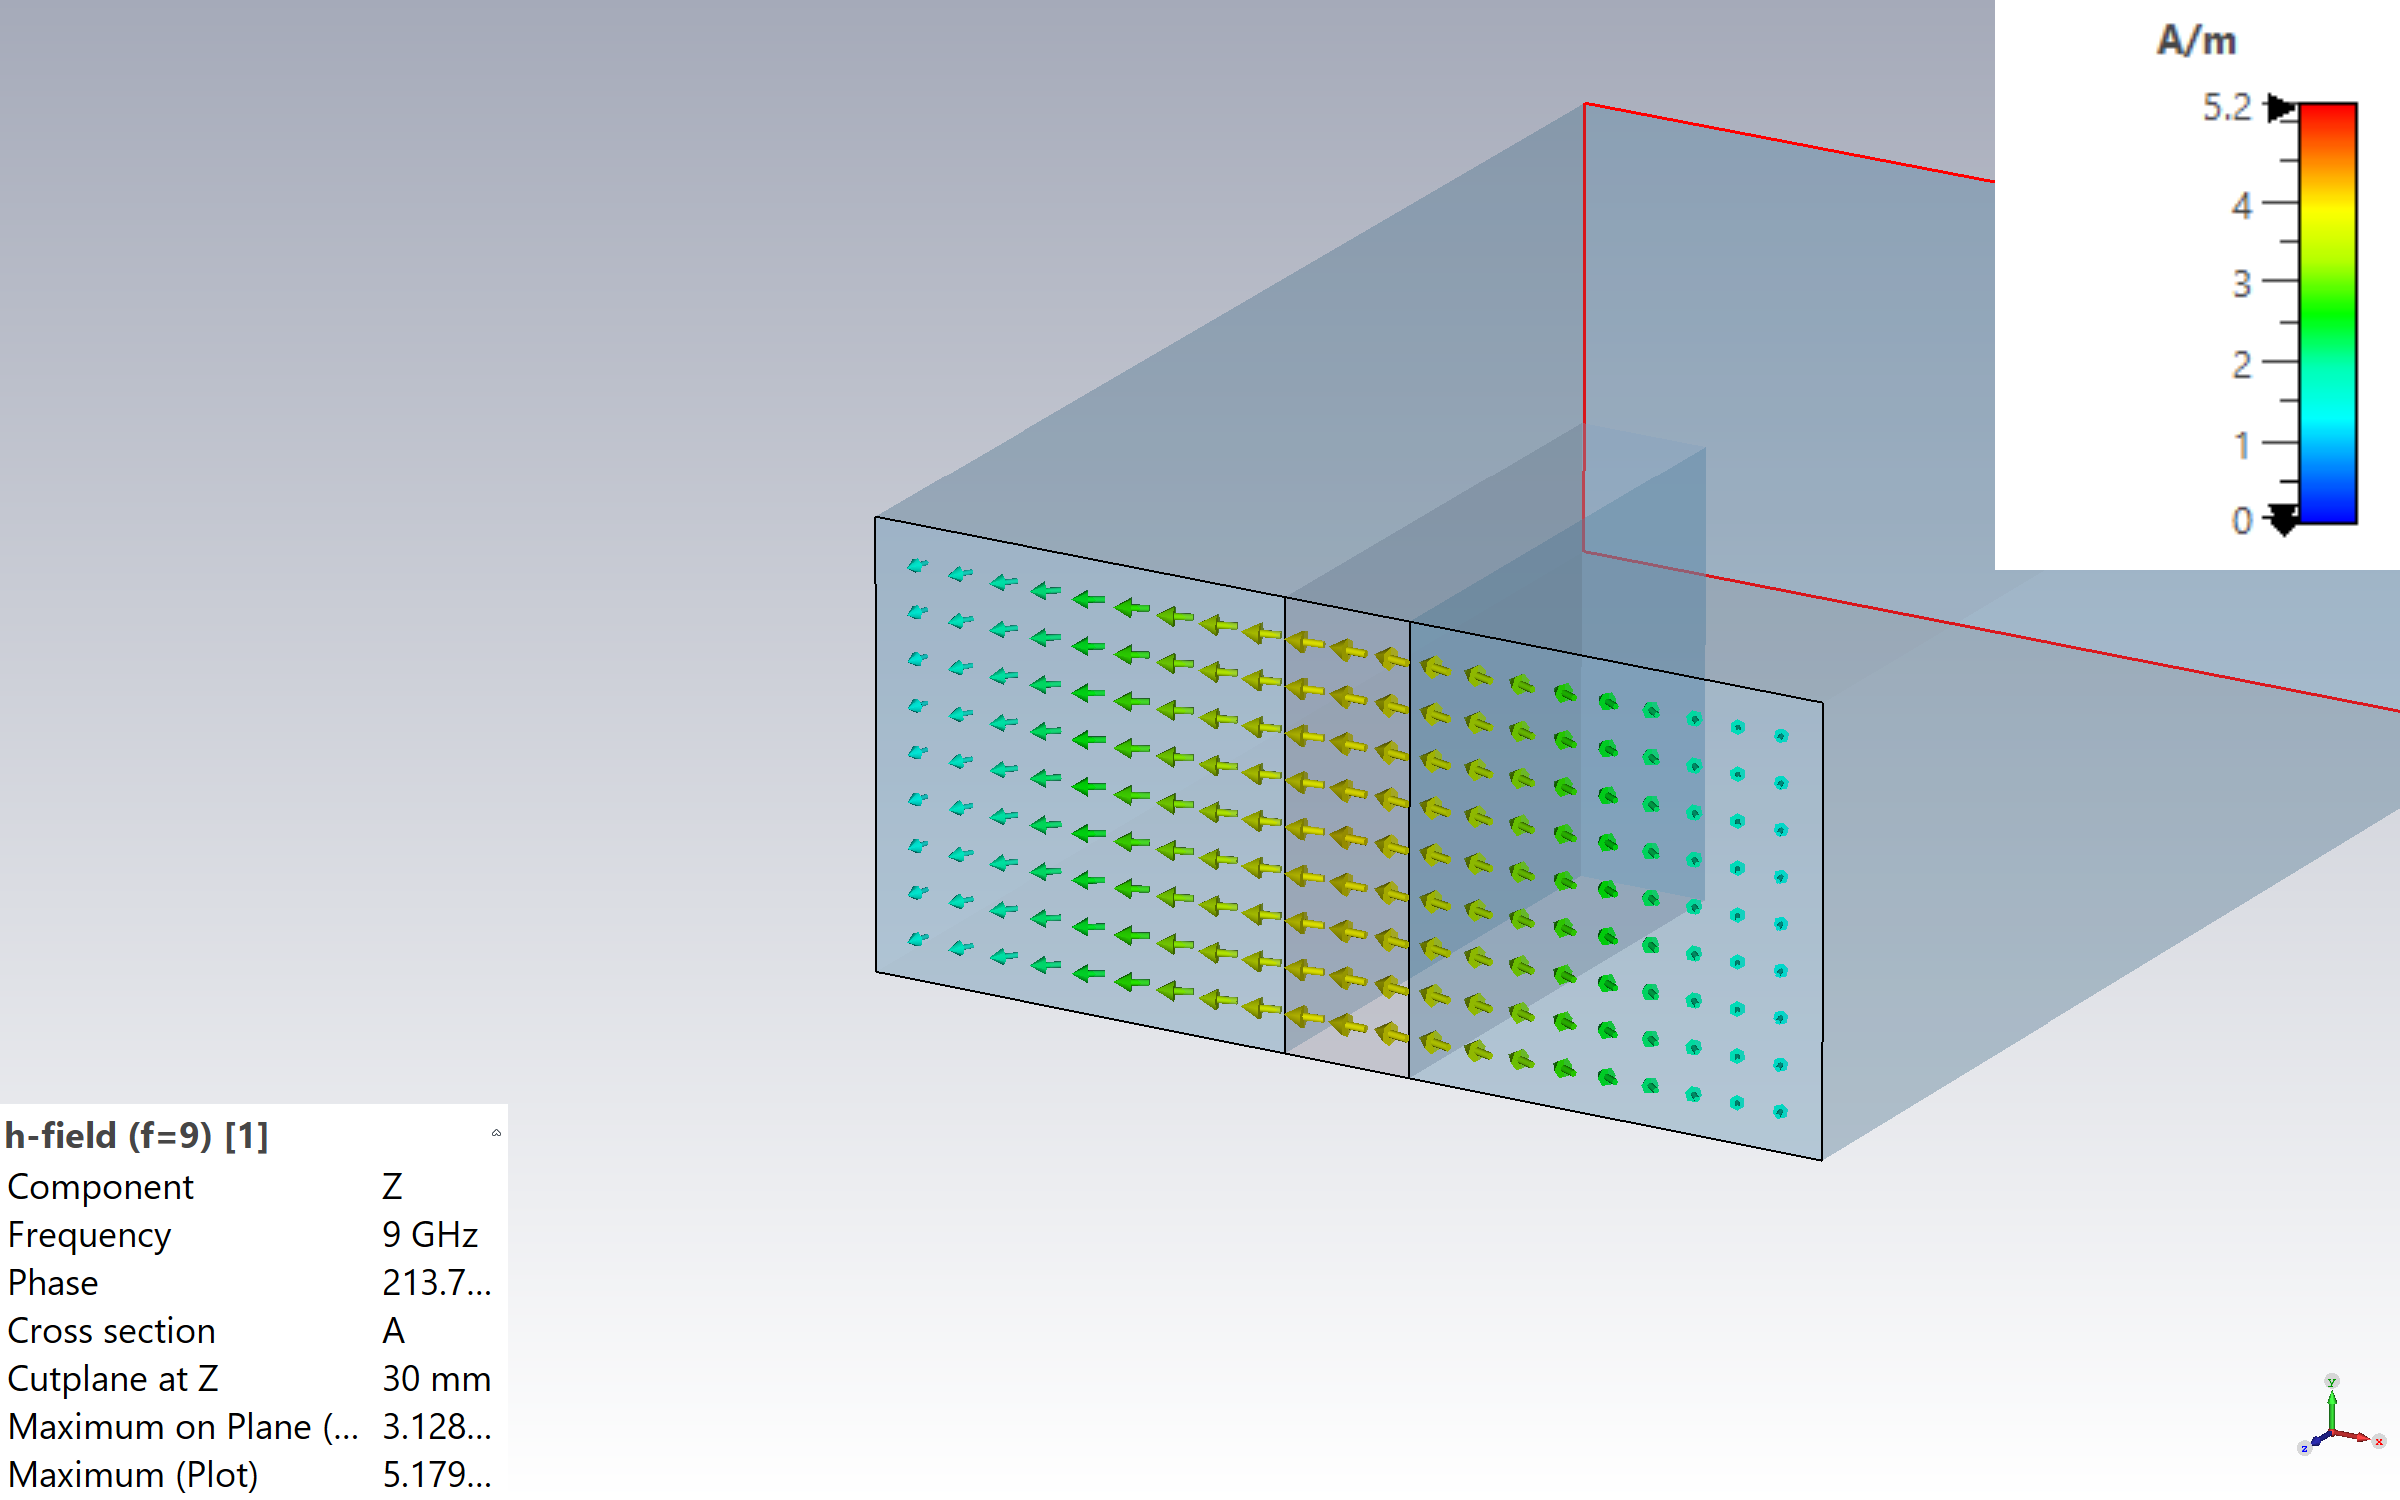
\includegraphics[width=\textwidth]{img/hfield_v2_vector_XY.png}
        \caption{میدان مغناطیسی --- نمای برداری}
    \end{subfigure}
    \hfill
    \begin{subfigure}[b]{0.48\textwidth}
        \centering
        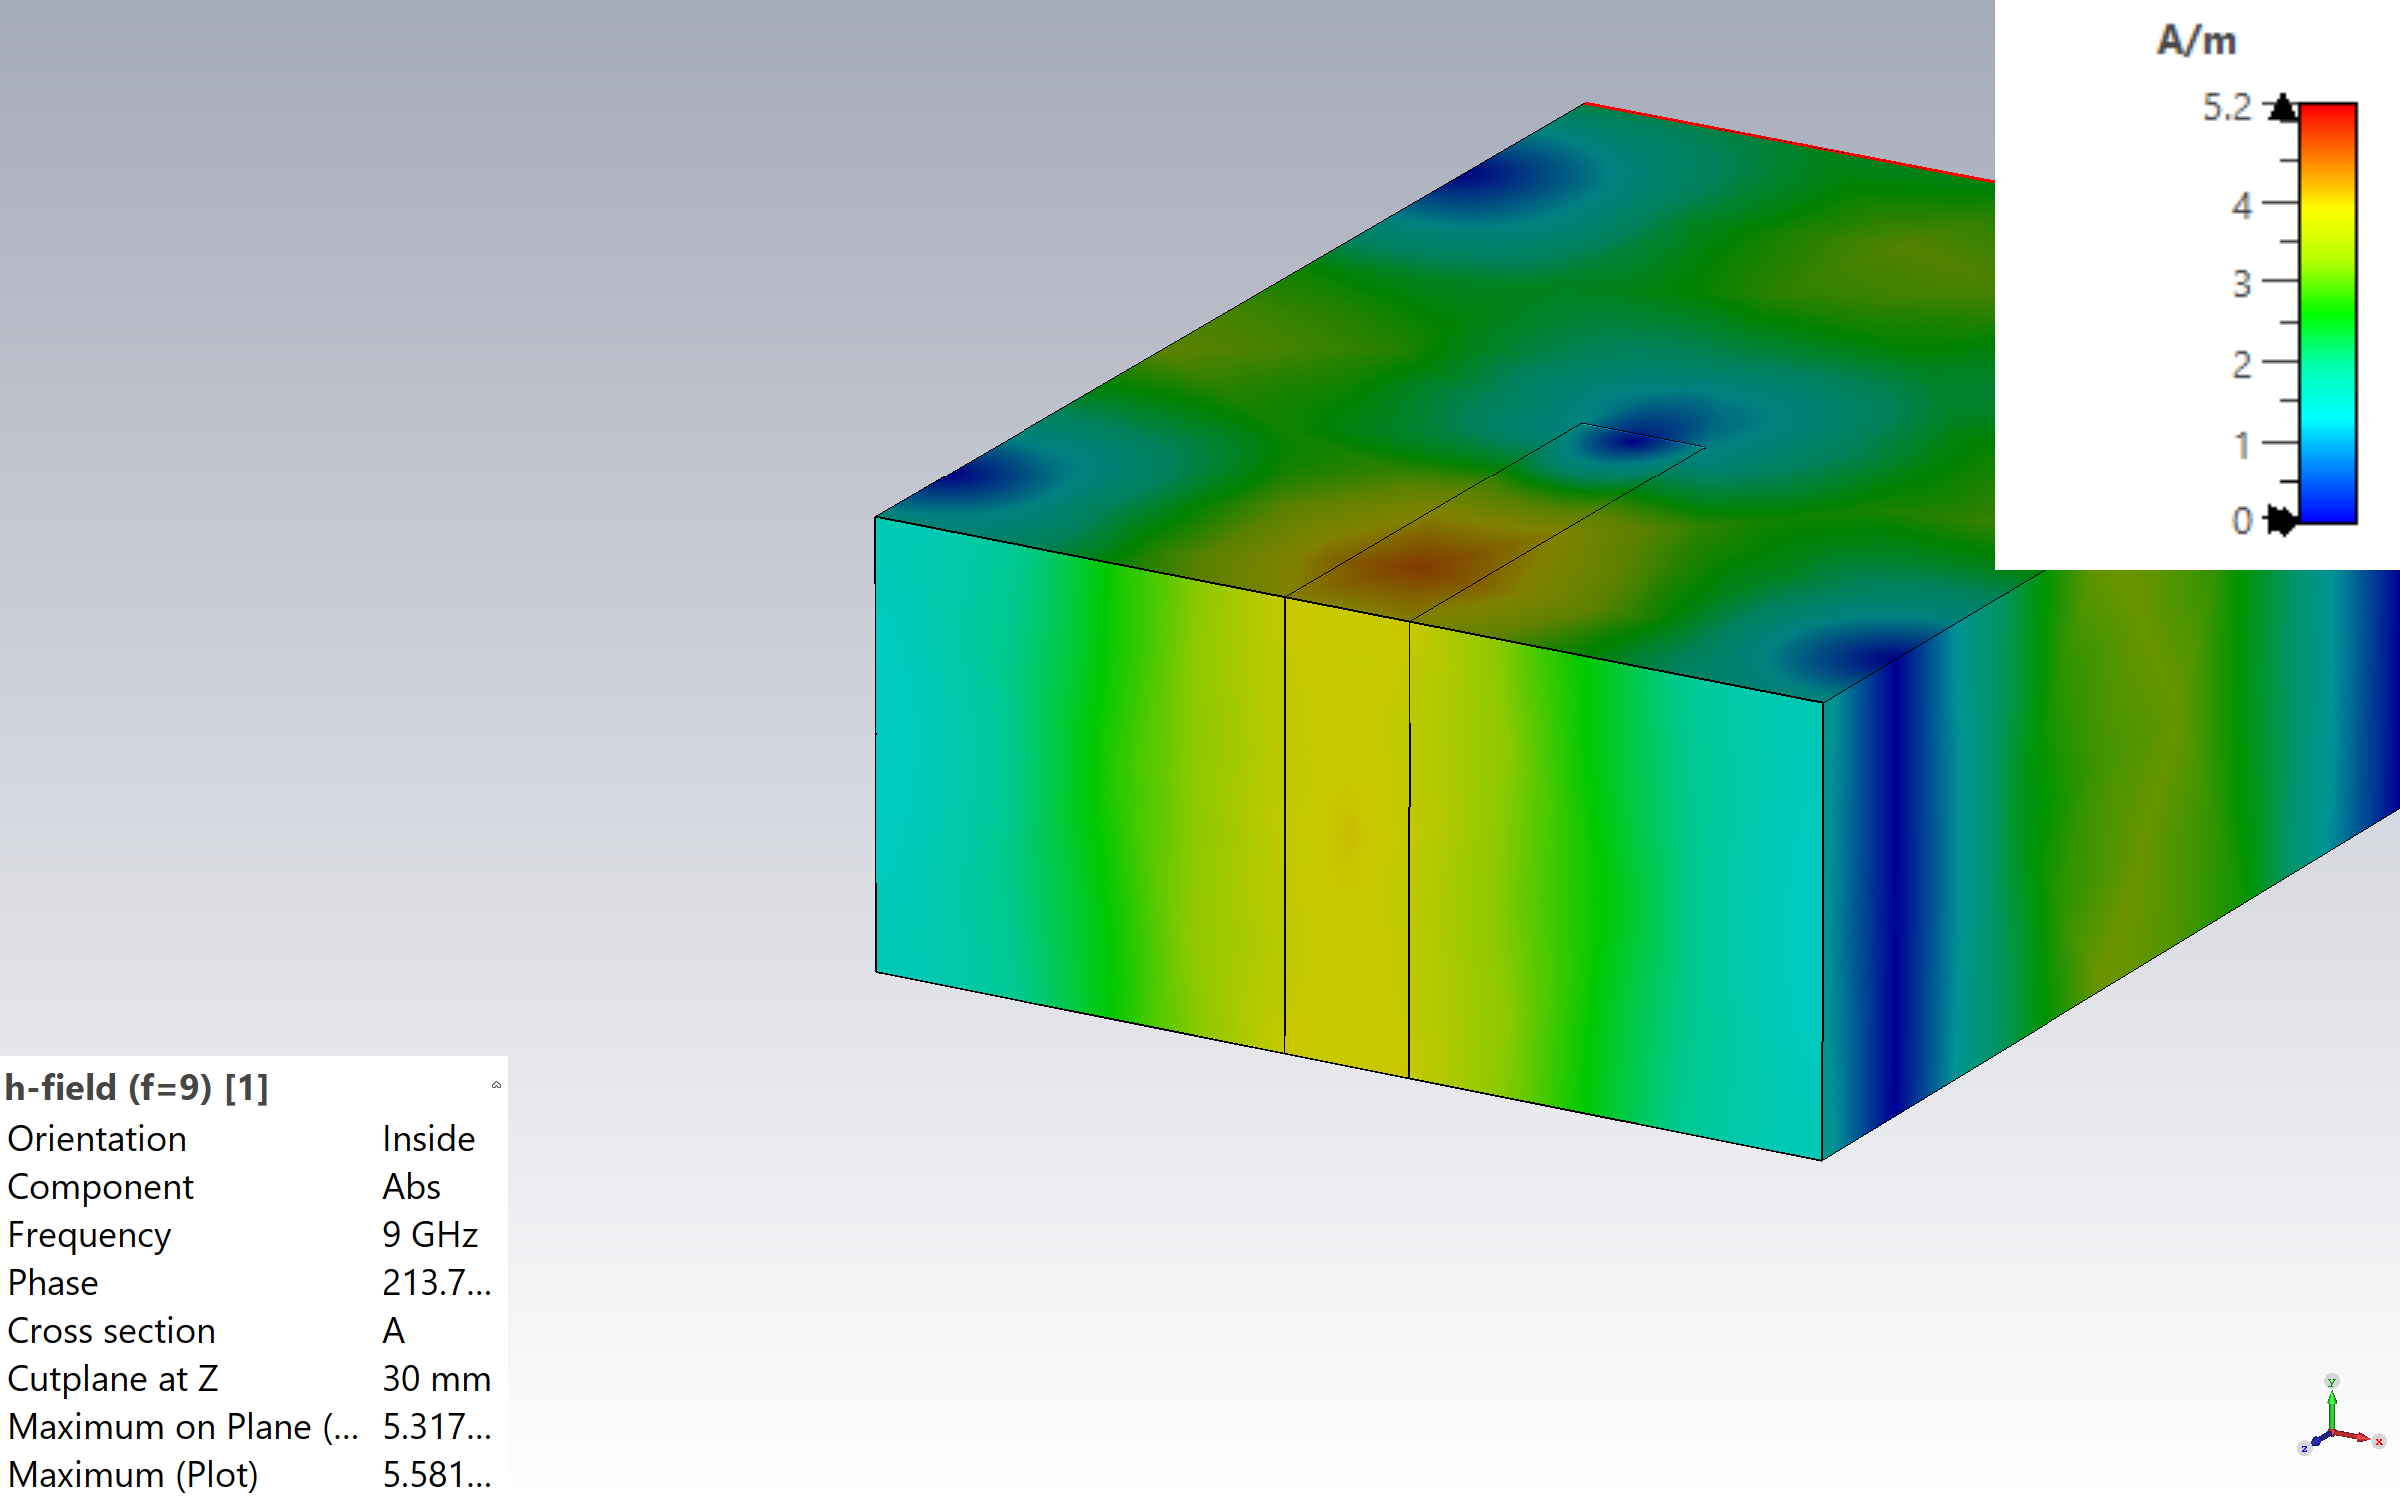
\includegraphics[width=\textwidth]{img/hfield_v2_contour_XY.png}
        \caption{میدان مغناطیسی --- نمای کانتوری پیوسته}
    \end{subfigure}
    \caption{توزیع میدان مغناطیسی در مقطع عرضی ($XY$) در $Z=30\text{ mm}$ (مقیاس یکنواخت: ۰ تا ۵٫۲ آمپر بر متر).}
    \label{fig:h_xy}
\end{figure}

همچنین در \autoref{fig:ey_transverse}، مقایسه تحلیلی پروفایل عرضی میدان الکتریکی موج‌بر خالی با ساختار بارگذاری‌شده با تیغه تفلون ارائه شده است که تمرکز بیشتر میدان در هسته دی‌الکتریک را نشان می‌دهد.

\begin{figure}[!htbp]
    \centering
    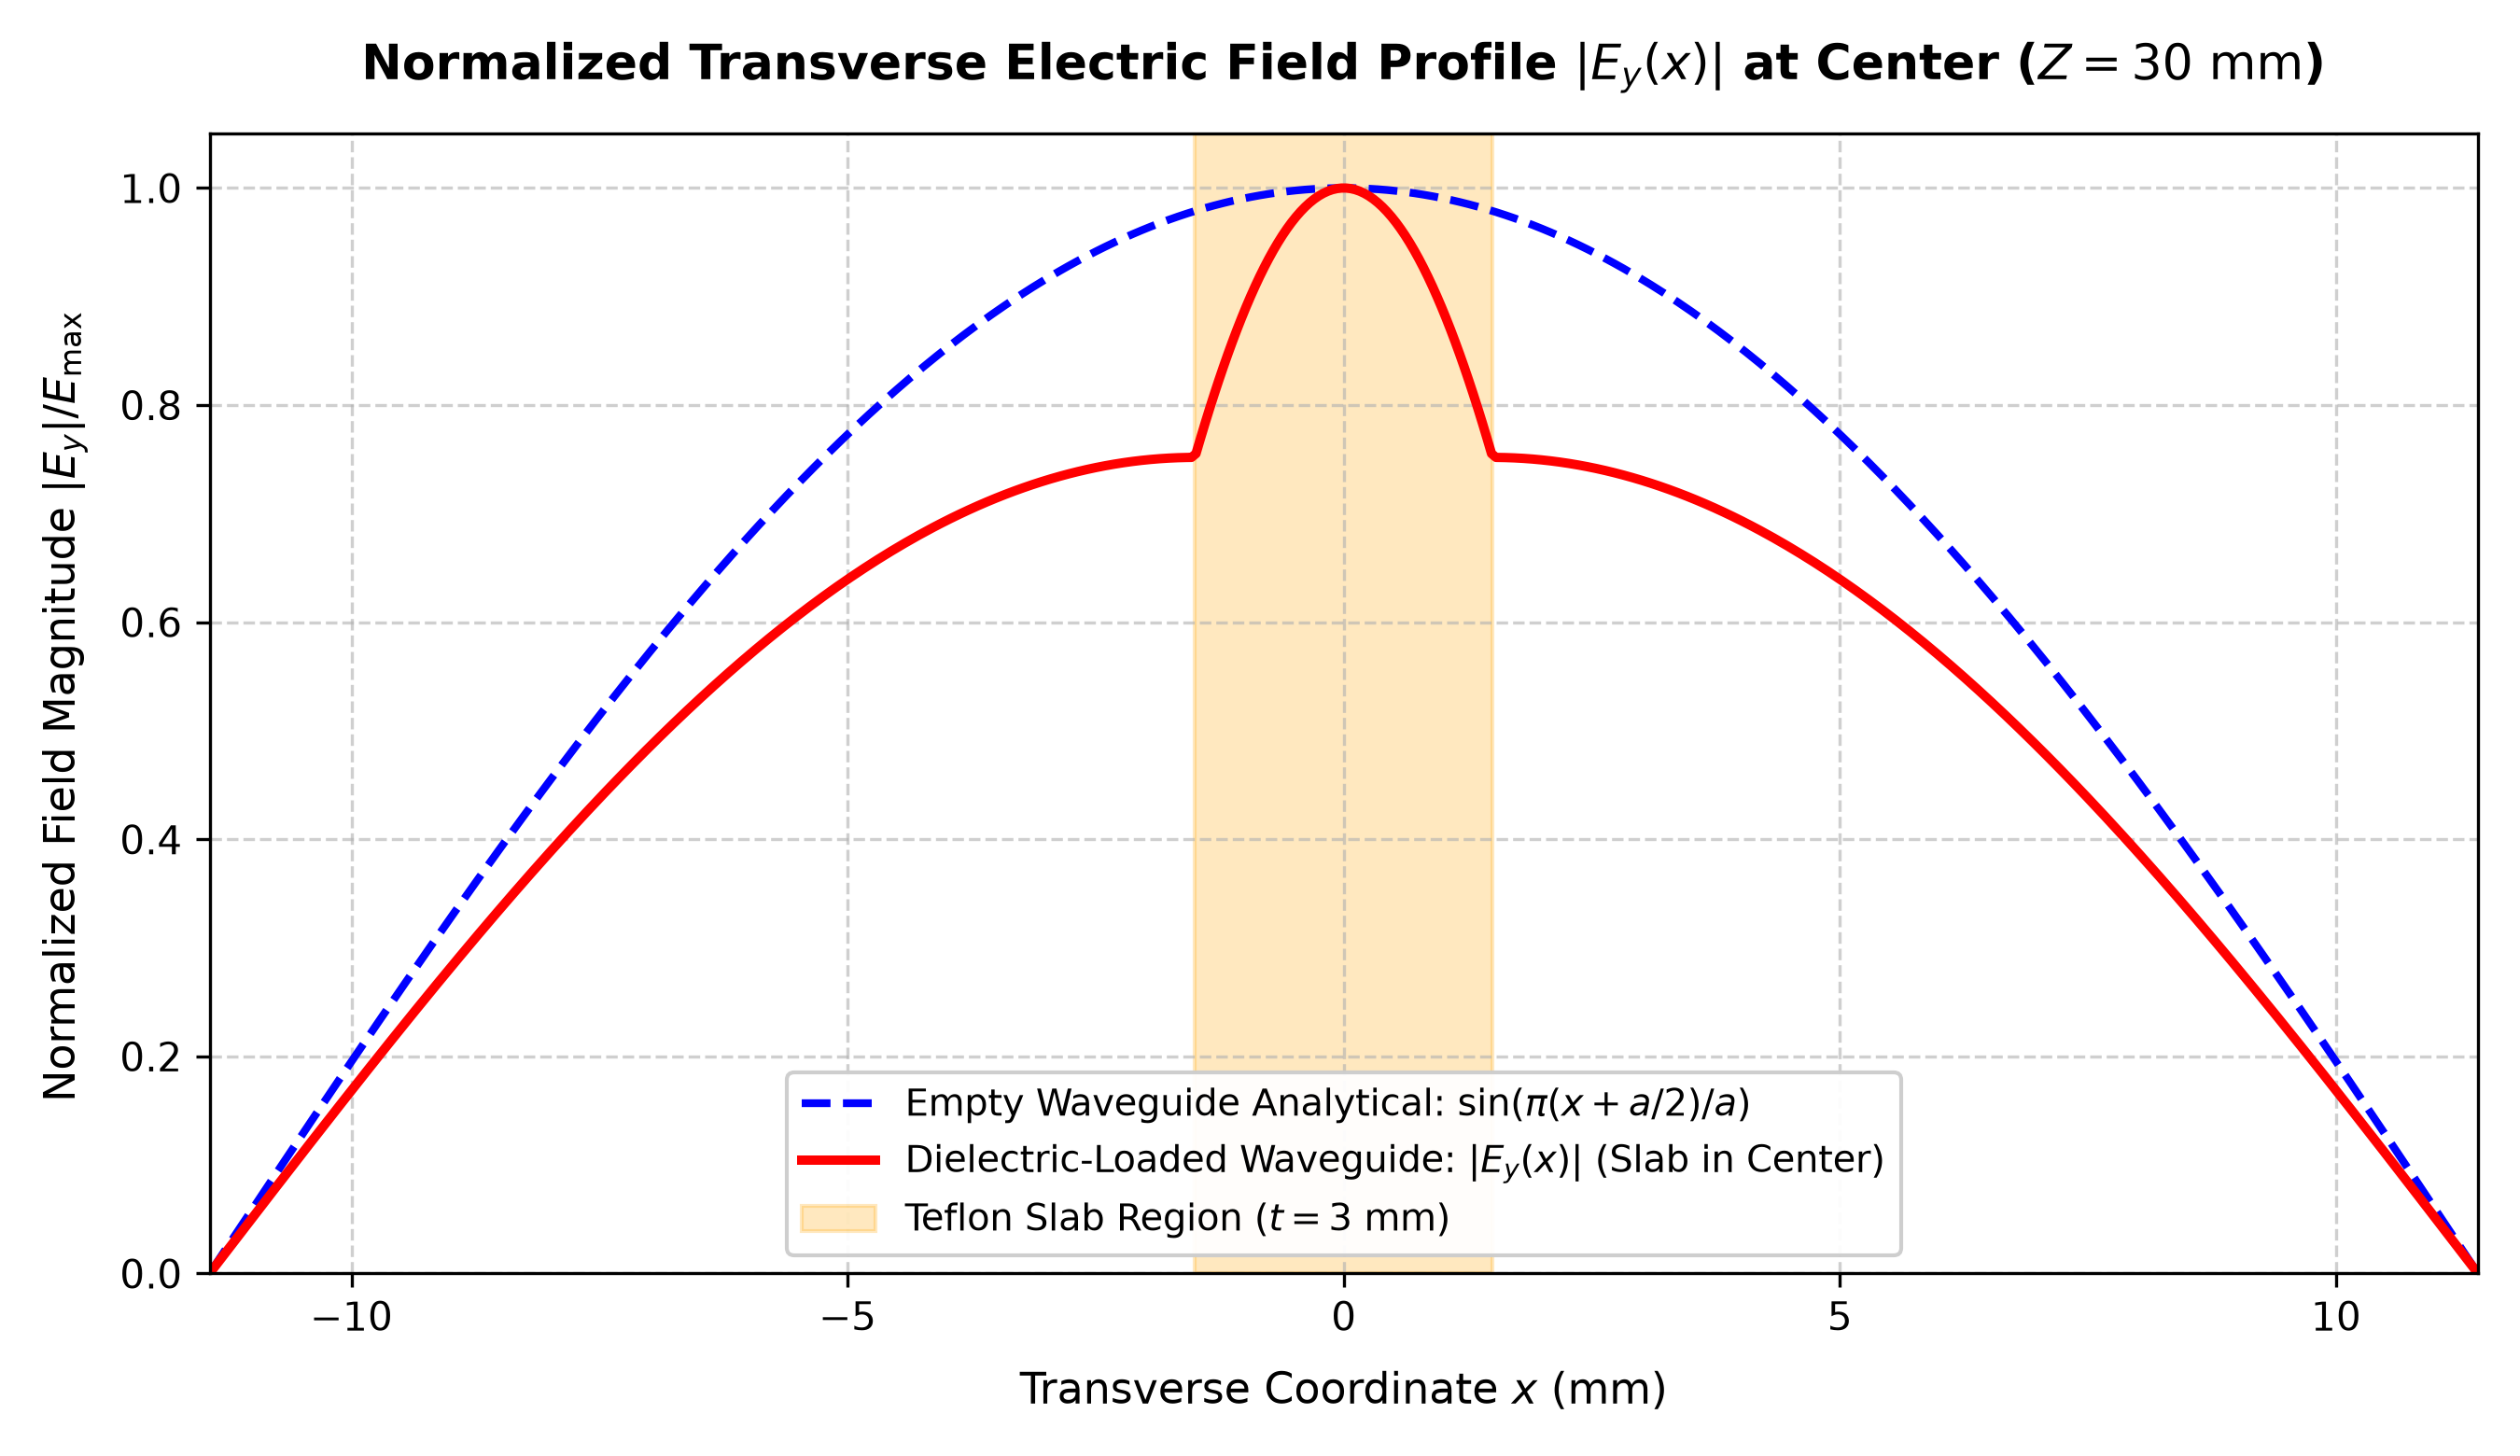
\includegraphics[width=0.85\textwidth]{img/ey_transverse_comparison.png}
    \caption{مقایسه پروفایل نرمال‌شده میدان $|E_y(x)|$ در مرکز موج‌بر بین حالت خالی ($\sin(\pi x/a)$) و تیغه‌دار.}
    \label{fig:ey_transverse}
\end{figure}

\subsection{صفحه طولی افقی ($XZ$) در $Y = 5.08\text{ mm}$}
برش طولی افقی رفتار انتشار امواج در امتداد محور Z را به تصویر می‌کشد. در هر دو نمای کانتوری و برداری، به وضوح دیده می‌شود که فاصله بین بیشینه‌ها و کمینه‌های متوالی میدان در ناحیه میانی موج‌بر (محدوده استقرار تیغه دی‌الکتریک از $Z=17.5\text{ mm}$ تا $Z=42.5\text{ mm}$) به صورت مشهود فشرده‌تر شده است. این فشرده‌سازی بازتاب مستقیم کاهش طول موج هدایت‌شده از $\lambda_{g0} = 48.63\text{ mm}$ به $\lambda_{g,\text{slab}} = 37.68\text{ mm}$ به دلیل افزایش ثابت فاز انتشار است. همچنین شدت رنگ‌های گرم‌تر و تراکم خطوط شار در هسته مرکزی نشان می‌دهد که دی‌الکتریک تفلون بخش عمده چگالی توان الکترومغناطیسی را در خود محبوس کرده است.

\begin{figure}[!htbp]
    \centering
    \begin{subfigure}[b]{0.48\textwidth}
        \centering
        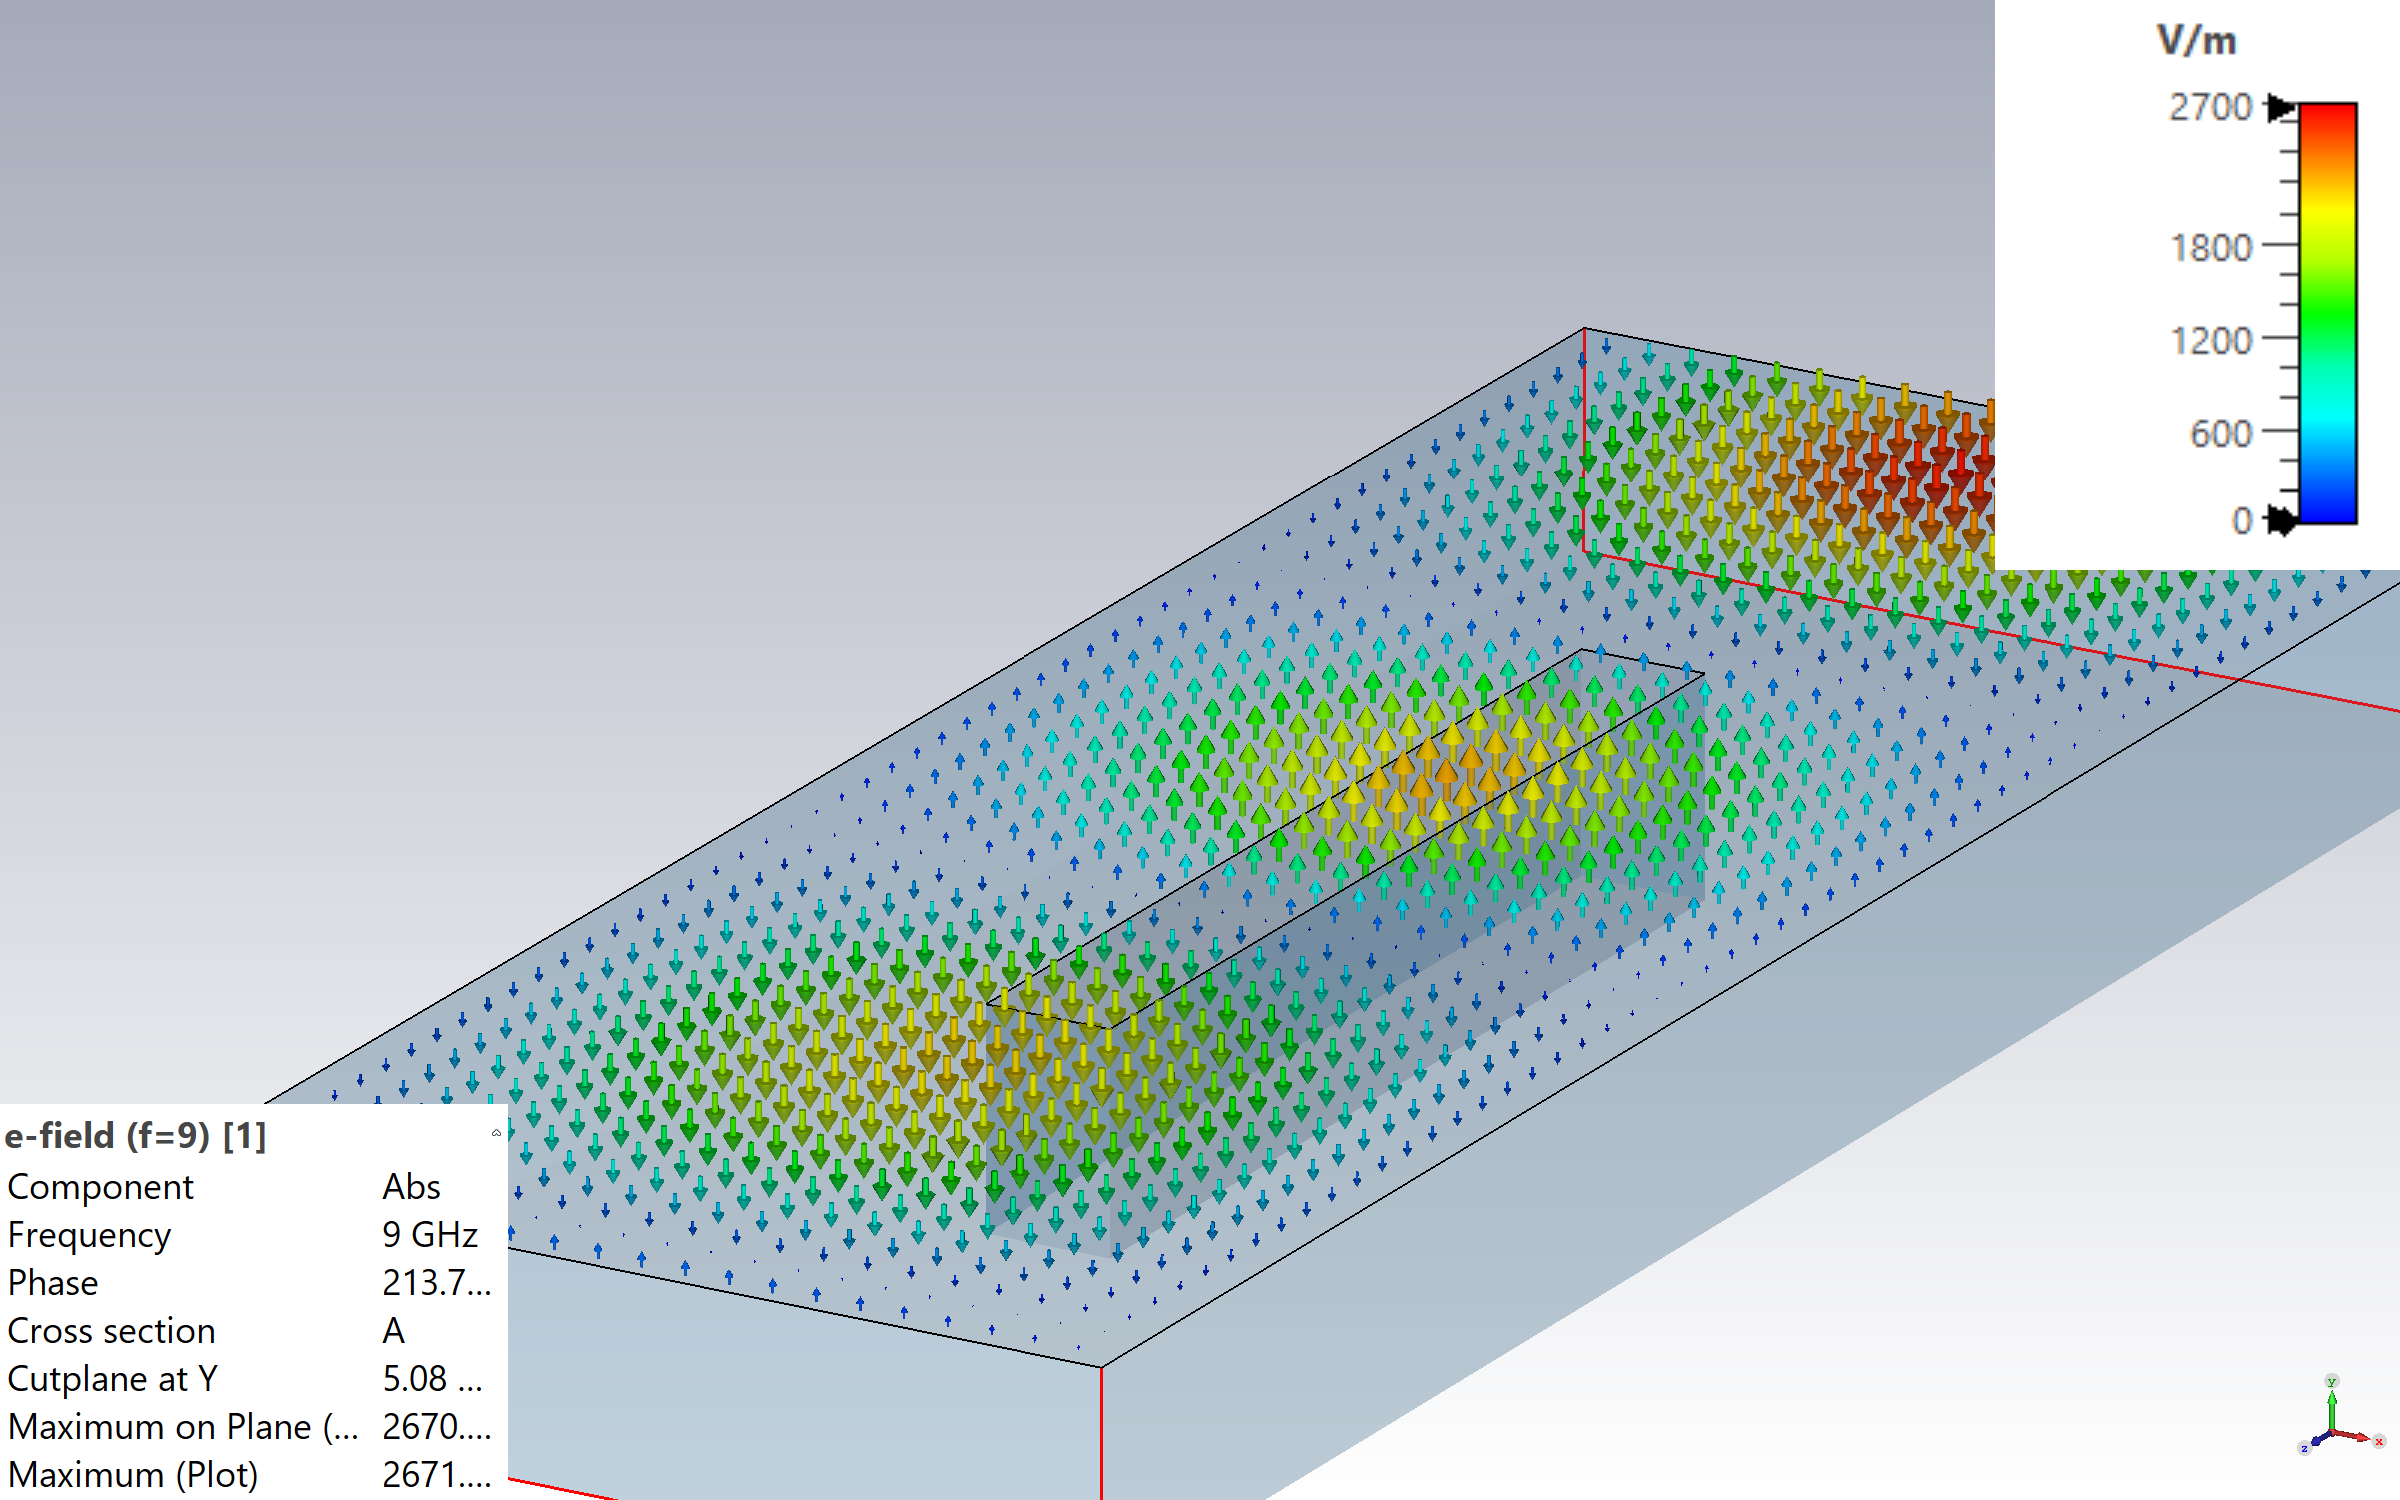
\includegraphics[width=\textwidth]{img/efield_v2_vector_XZ.png}
        \caption{میدان الکتریکی --- نمای برداری}
    \end{subfigure}
    \hfill
    \begin{subfigure}[b]{0.48\textwidth}
        \centering
        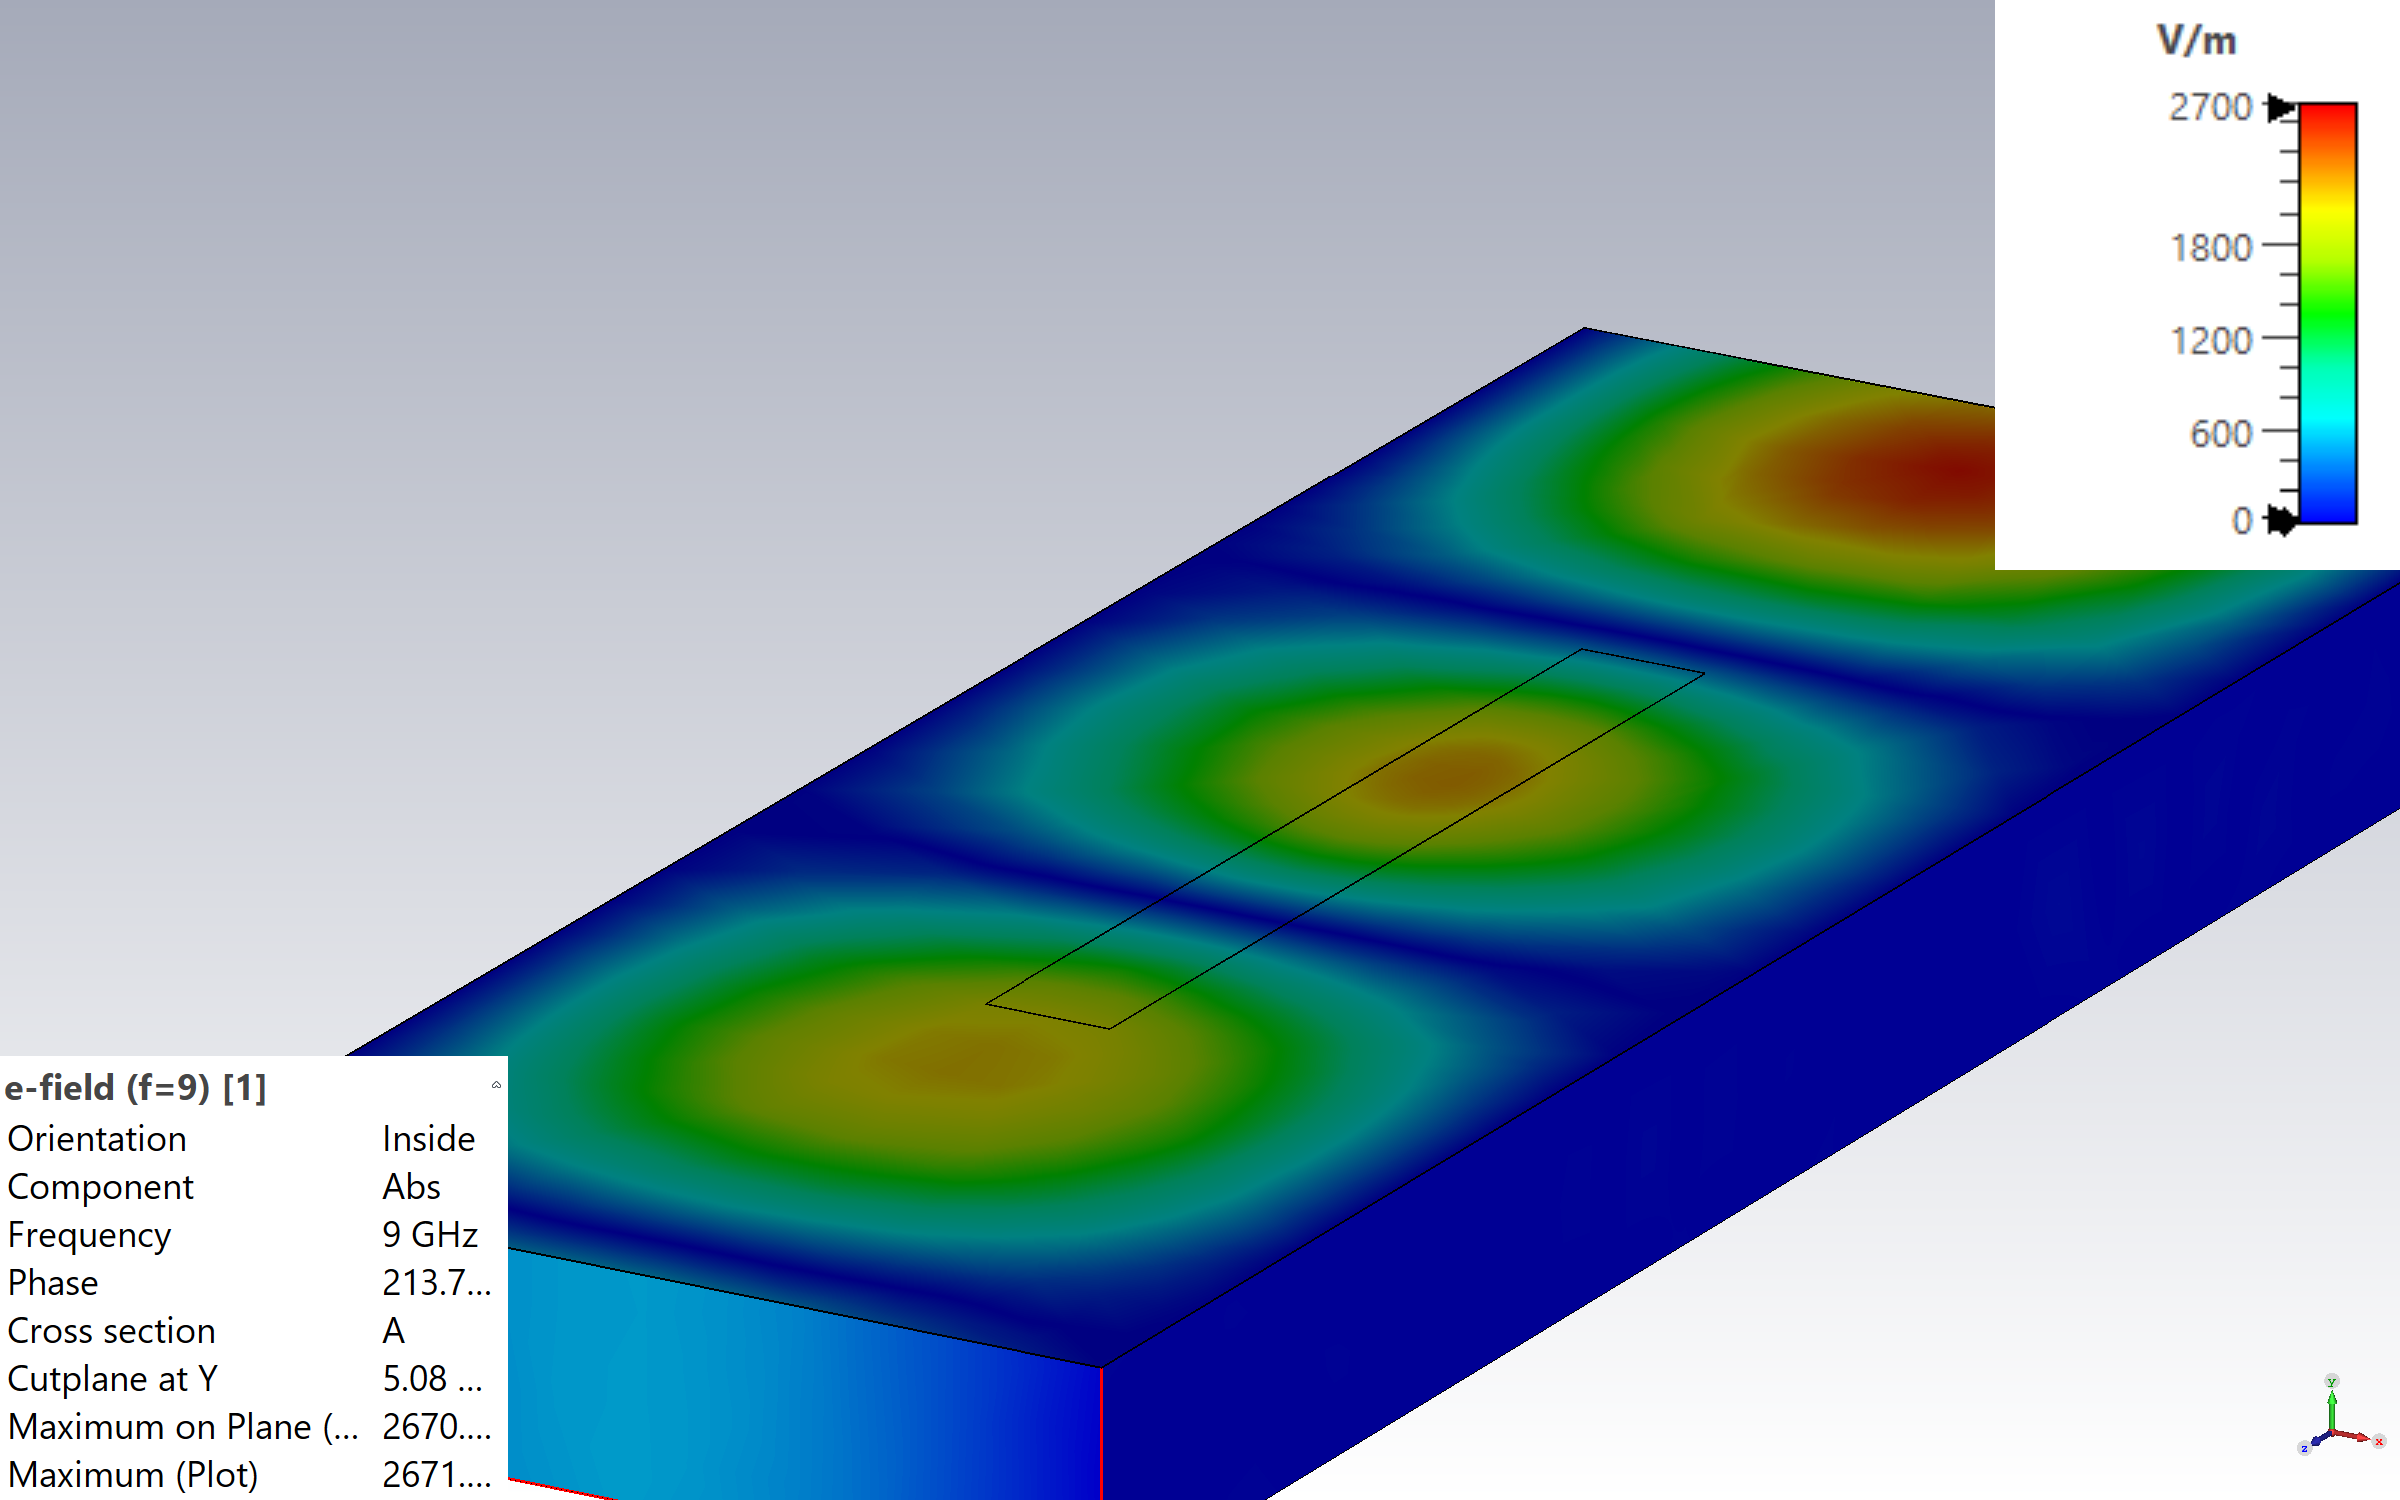
\includegraphics[width=\textwidth]{img/efield_v2_contour_XZ.png}
        \caption{میدان الکتریکی --- نمای کانتوری پیوسته}
    \end{subfigure}
    \caption{توزیع میدان الکتریکی در صفحه طولی افقی ($XZ$) در $Y=5.08\text{ mm}$ (مقیاس: ۰ تا ۲۷۰۰ ولت بر متر).}
    \label{fig:e_xz}
\end{figure}

\begin{figure}[!htbp]
    \centering
    \begin{subfigure}[b]{0.48\textwidth}
        \centering
        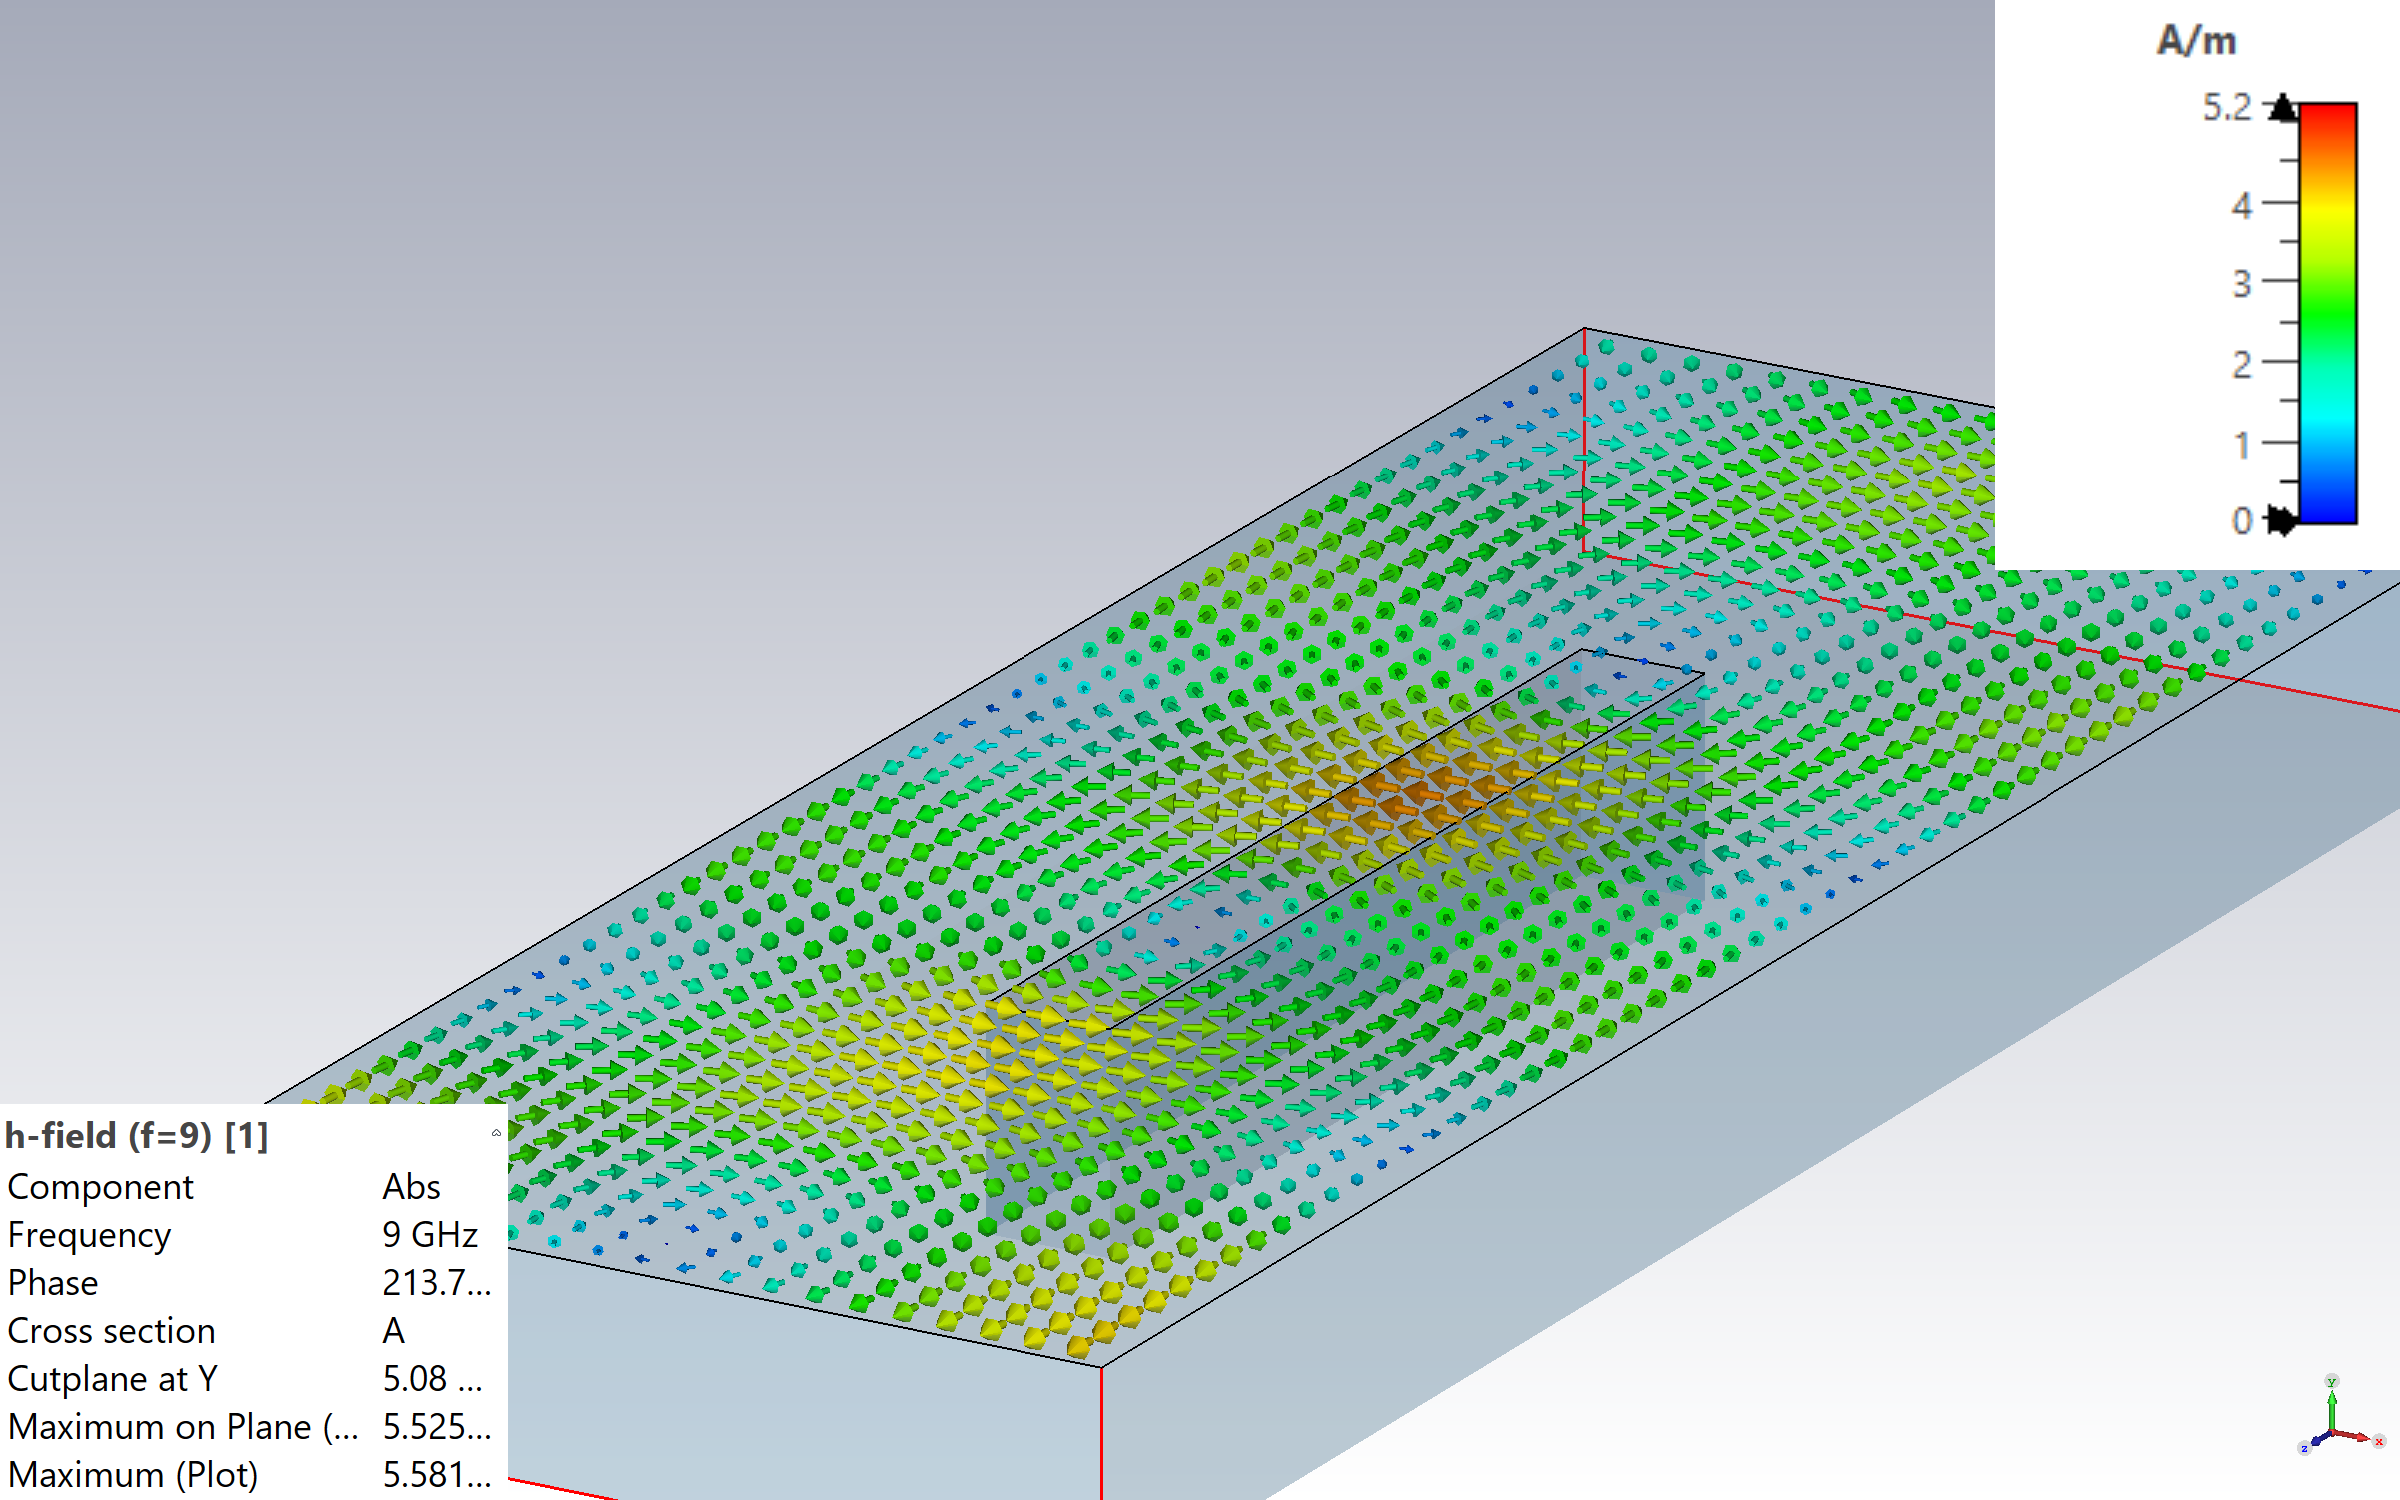
\includegraphics[width=\textwidth]{img/hfield_v2_vector_XZ.png}
        \caption{میدان مغناطیسی --- نمای برداری}
    \end{subfigure}
    \hfill
    \begin{subfigure}[b]{0.48\textwidth}
        \centering
        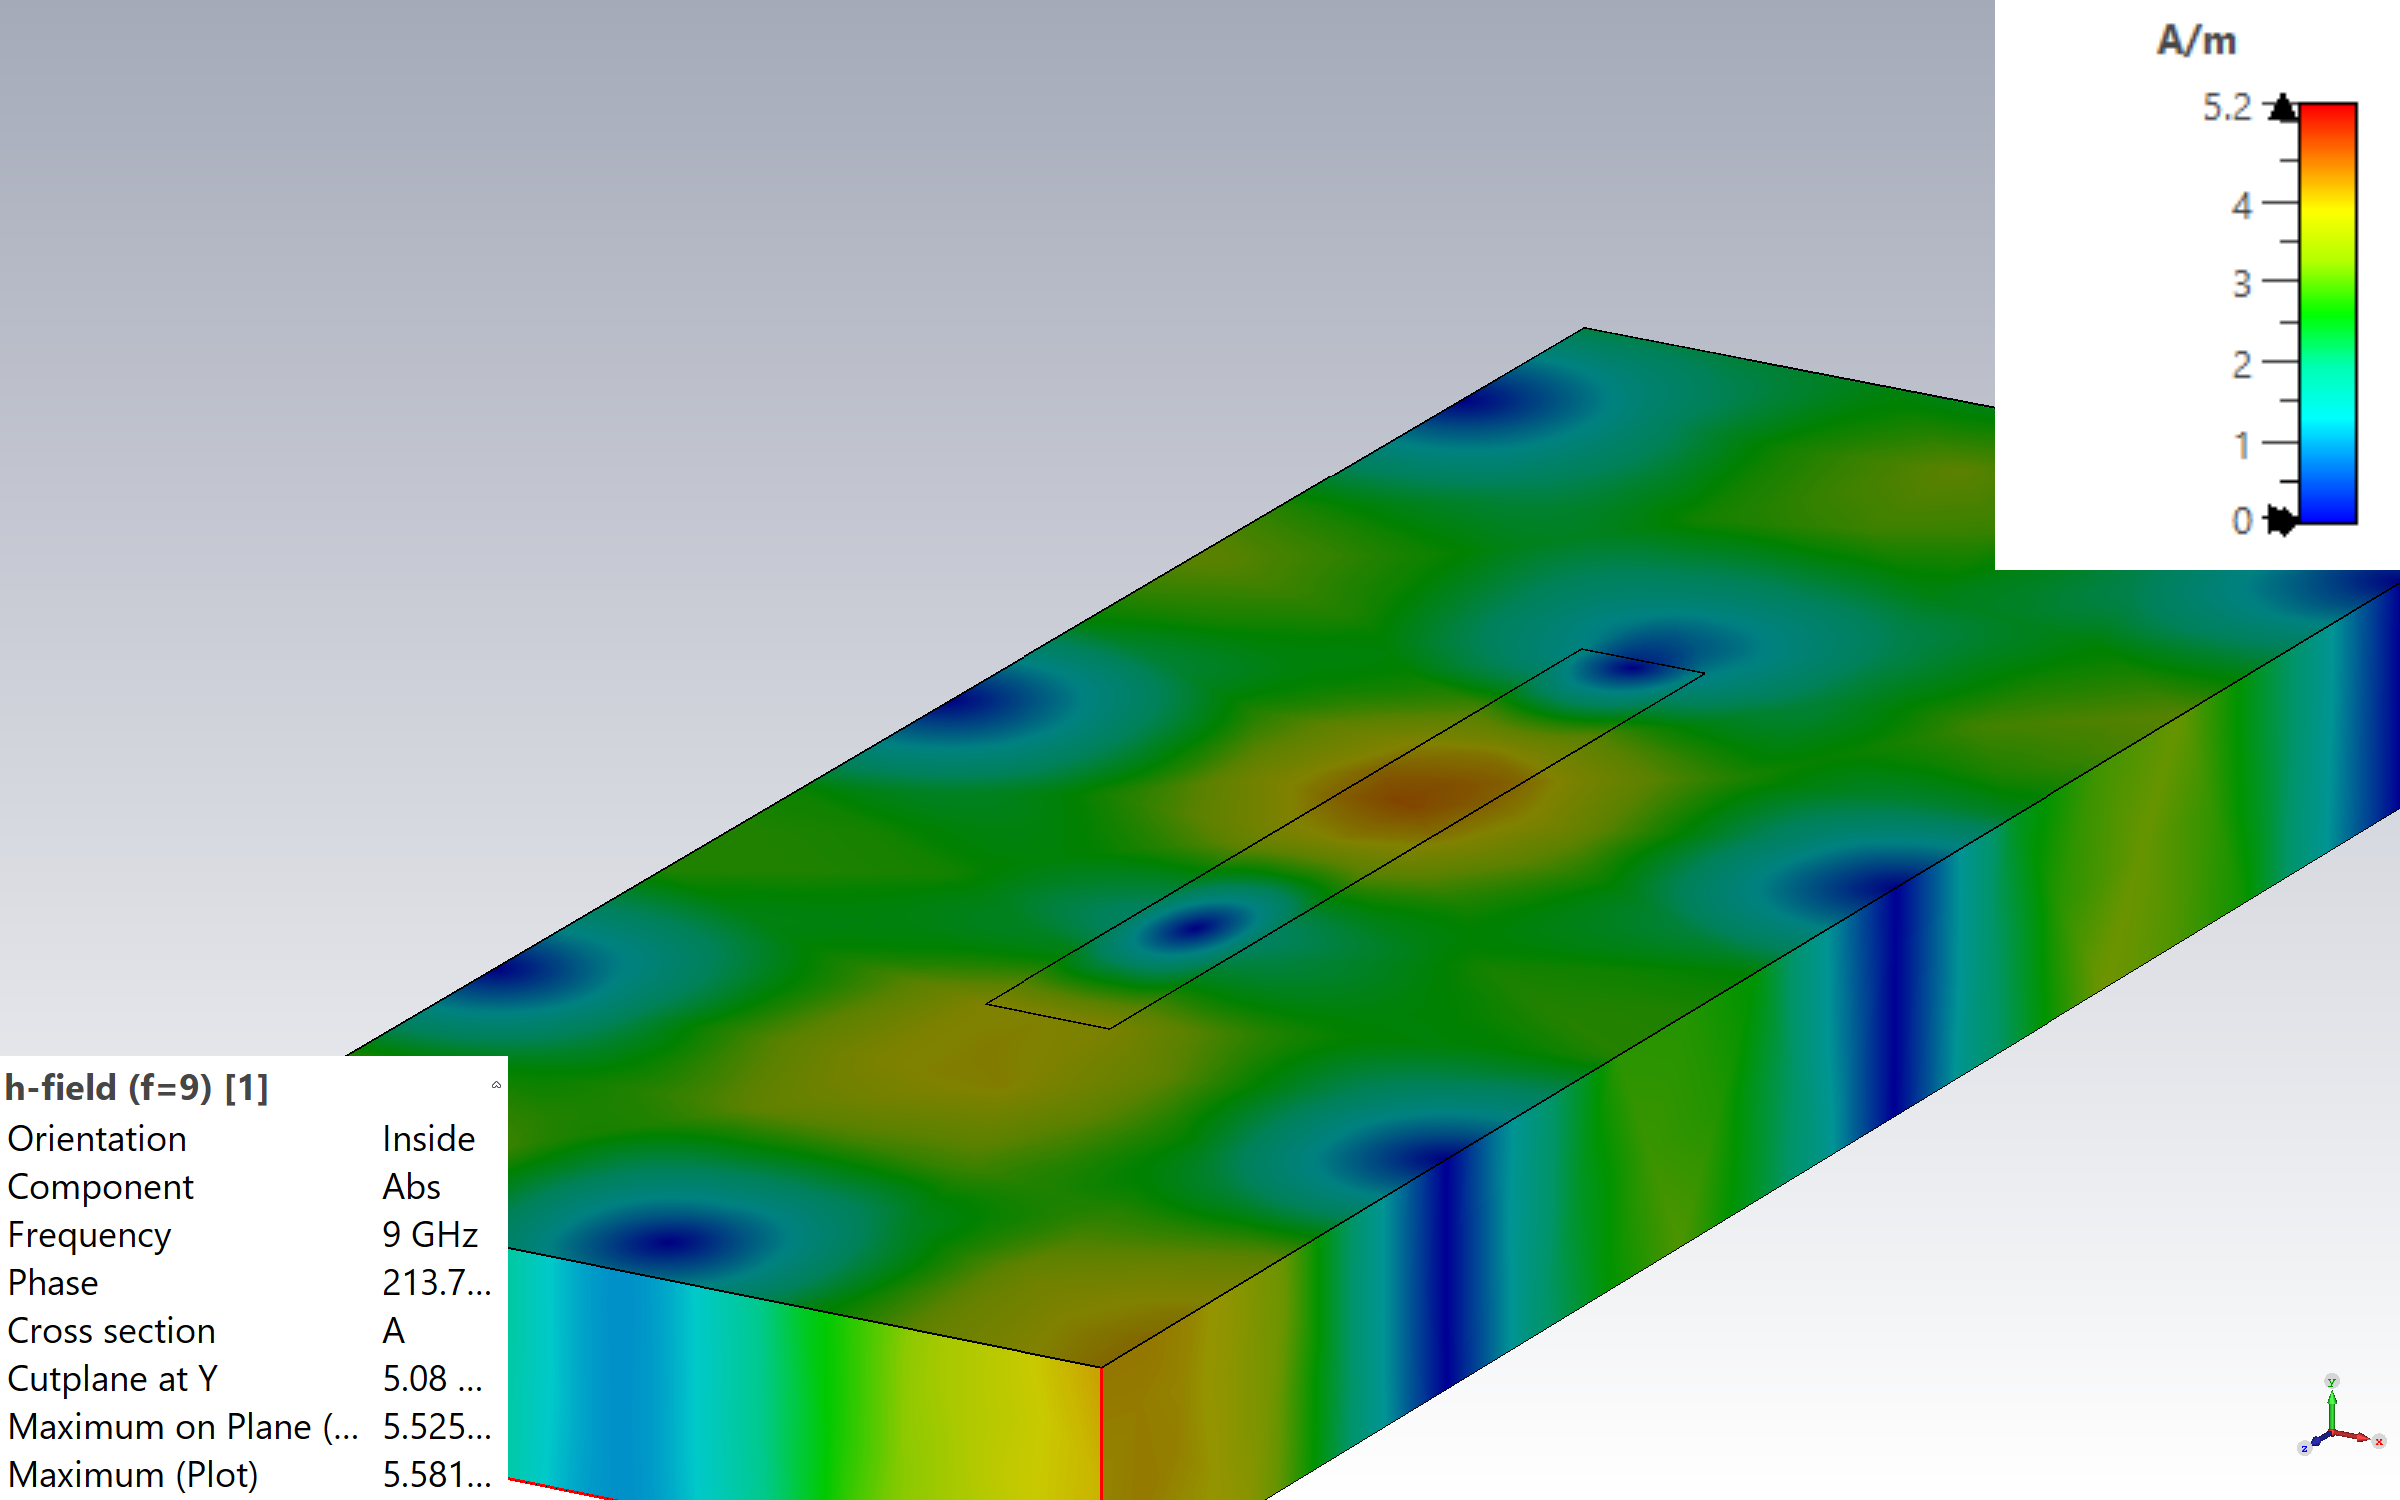
\includegraphics[width=\textwidth]{img/hfield_v2_contour_XZ.png}
        \caption{میدان مغناطیسی --- نمای کانتوری پیوسته}
    \end{subfigure}
    \caption{توزیع میدان مغناطیسی در صفحه طولی افقی ($XZ$) در $Y=5.08\text{ mm}$ (مقیاس: ۰ تا ۵٫۲ آمپر بر متر).}
    \label{fig:h_xz}
\end{figure}

\subsection{صفحه طولی عمودی ($YZ$) در $X = 0\text{ mm}$}
در صفحه تقارن عمودی ($X=0$)، توزیع میدان در امتداد ارتفاع موج‌بر مورد بررسی قرار می‌گیرد. در نمای کانتوری، نوارهای رنگی کاملاً یکدست و موازی با محور افقی هستند و هیچ‌گونه تغییرات گرادیانی در امتداد بعد عمودی $y$ مشاهده نمی‌شود. این یکنواختی عمودی تایید می‌کند که مد منتشره دقیقاً مد $\text{TE}_{10}$ با شاخص ارتفاعی صفر ($n=0$) است و هیچ مد مرتبه بالاتری نظیر $\text{TE}_{01}$ برانگیخته نشده است. فلش‌های برداری در تمام ارتفاع اندازه و جهت ثابتی به سمت بالا دارند که نشان‌دهنده ارضای طبیعی شرایط مرزی روی دیواره‌های بالا و پایین هادی ایده‌آل است.

\begin{figure}[!htbp]
    \centering
    \begin{subfigure}[b]{0.48\textwidth}
        \centering
        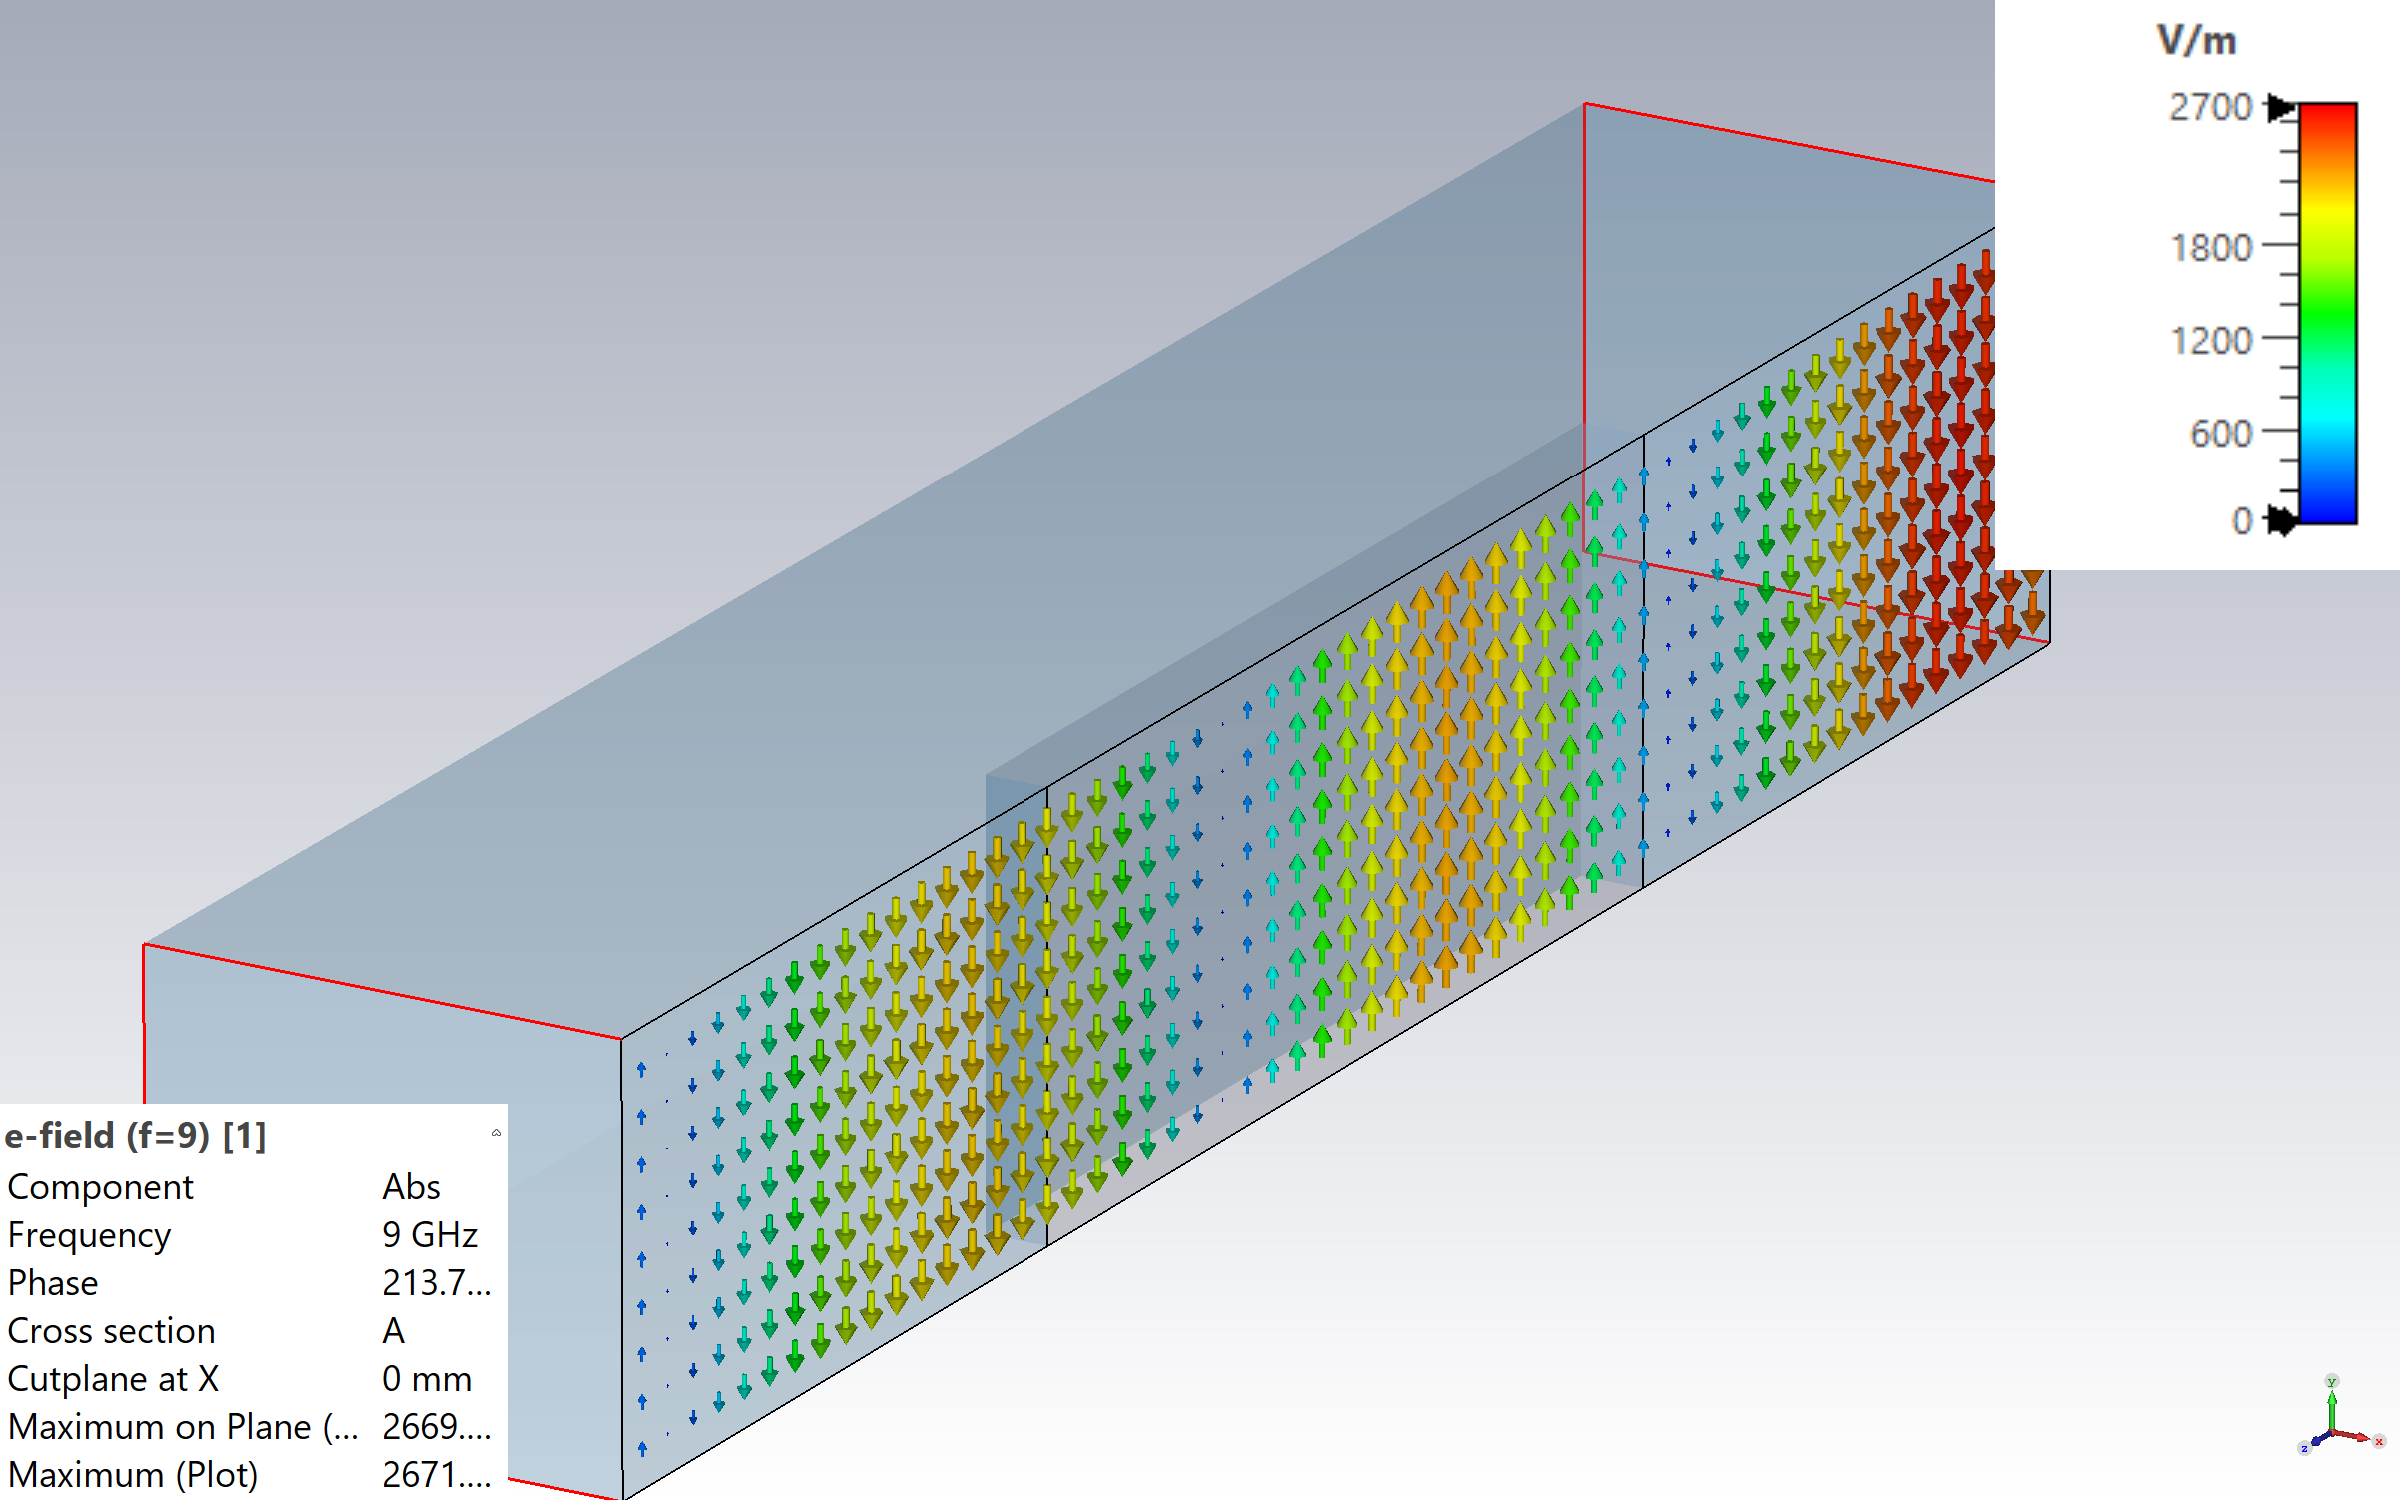
\includegraphics[width=\textwidth]{img/efield_v2_vector_YZ.png}
        \caption{میدان الکتریکی --- نمای برداری}
    \end{subfigure}
    \hfill
    \begin{subfigure}[b]{0.48\textwidth}
        \centering
        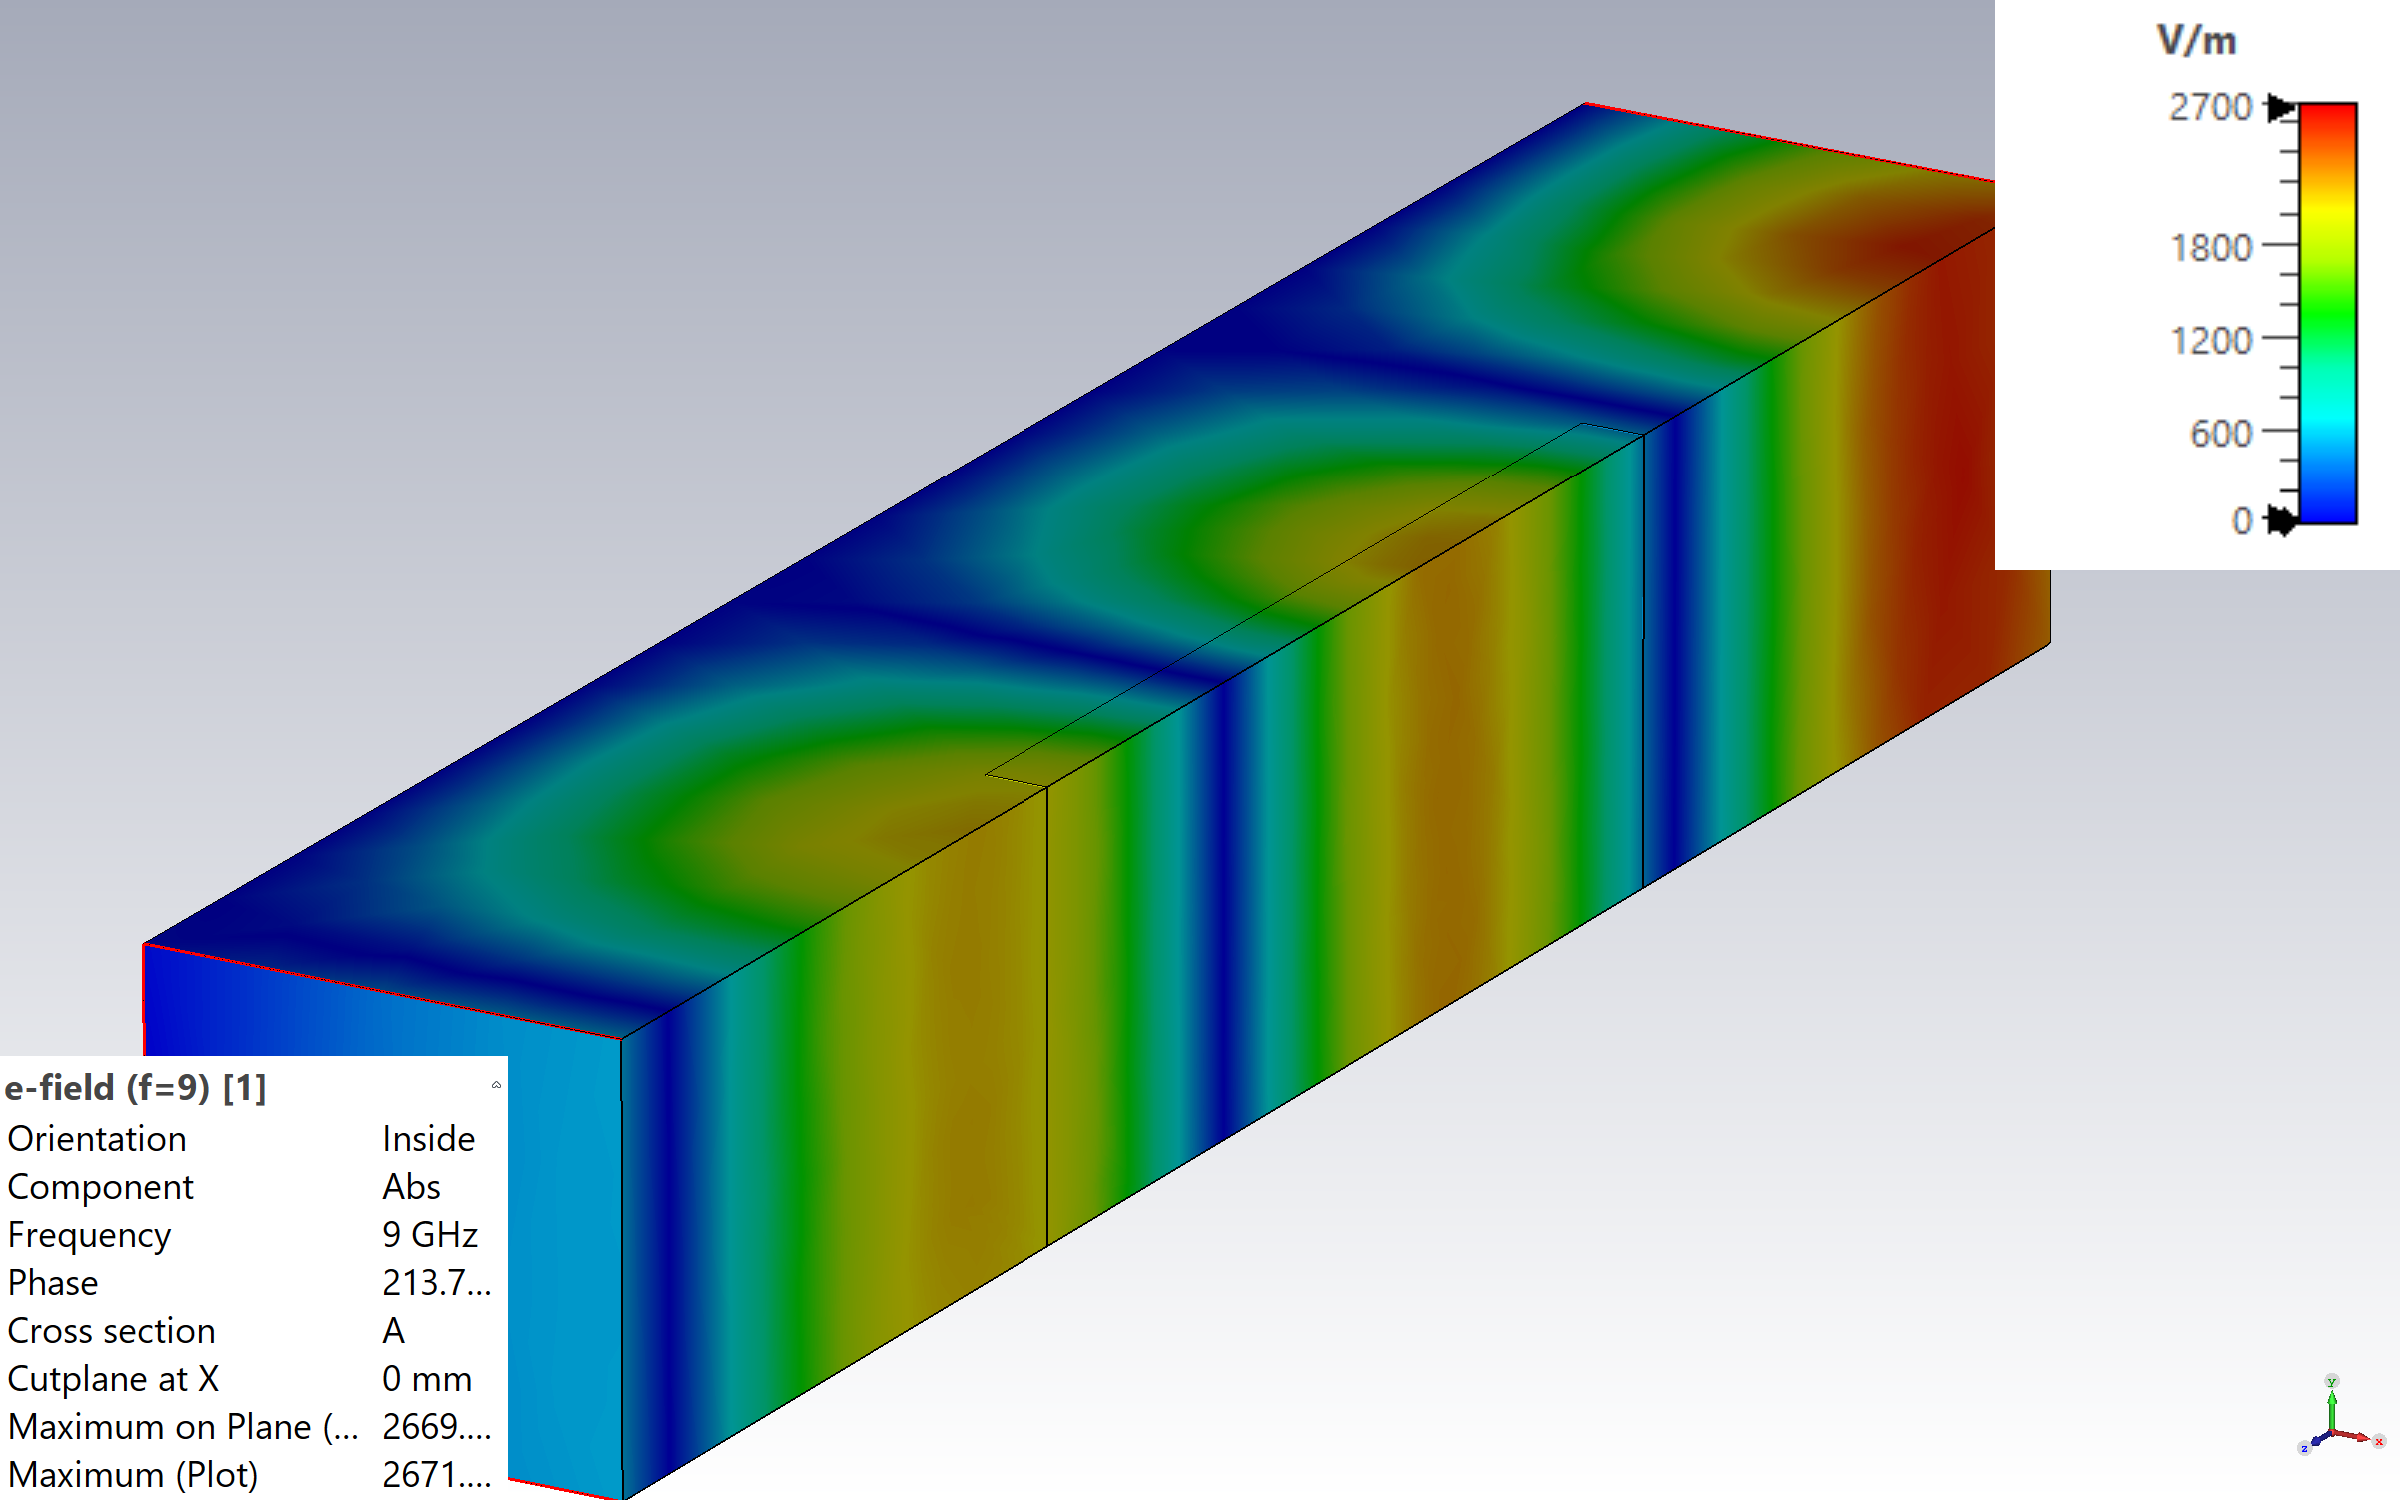
\includegraphics[width=\textwidth]{img/efield_v2_contour_YZ.png}
        \caption{میدان الکتریکی --- نمای کانتوری پیوسته}
    \end{subfigure}
    \caption{توزیع میدان الکتریکی در صفحه طولی عمودی ($YZ$) در $X=0\text{ mm}$ (مقیاس: ۰ تا ۲۷۰۰ ولت بر متر).}
    \label{fig:e_yz}
\end{figure}

\begin{figure}[!htbp]
    \centering
    \begin{subfigure}[b]{0.48\textwidth}
        \centering
        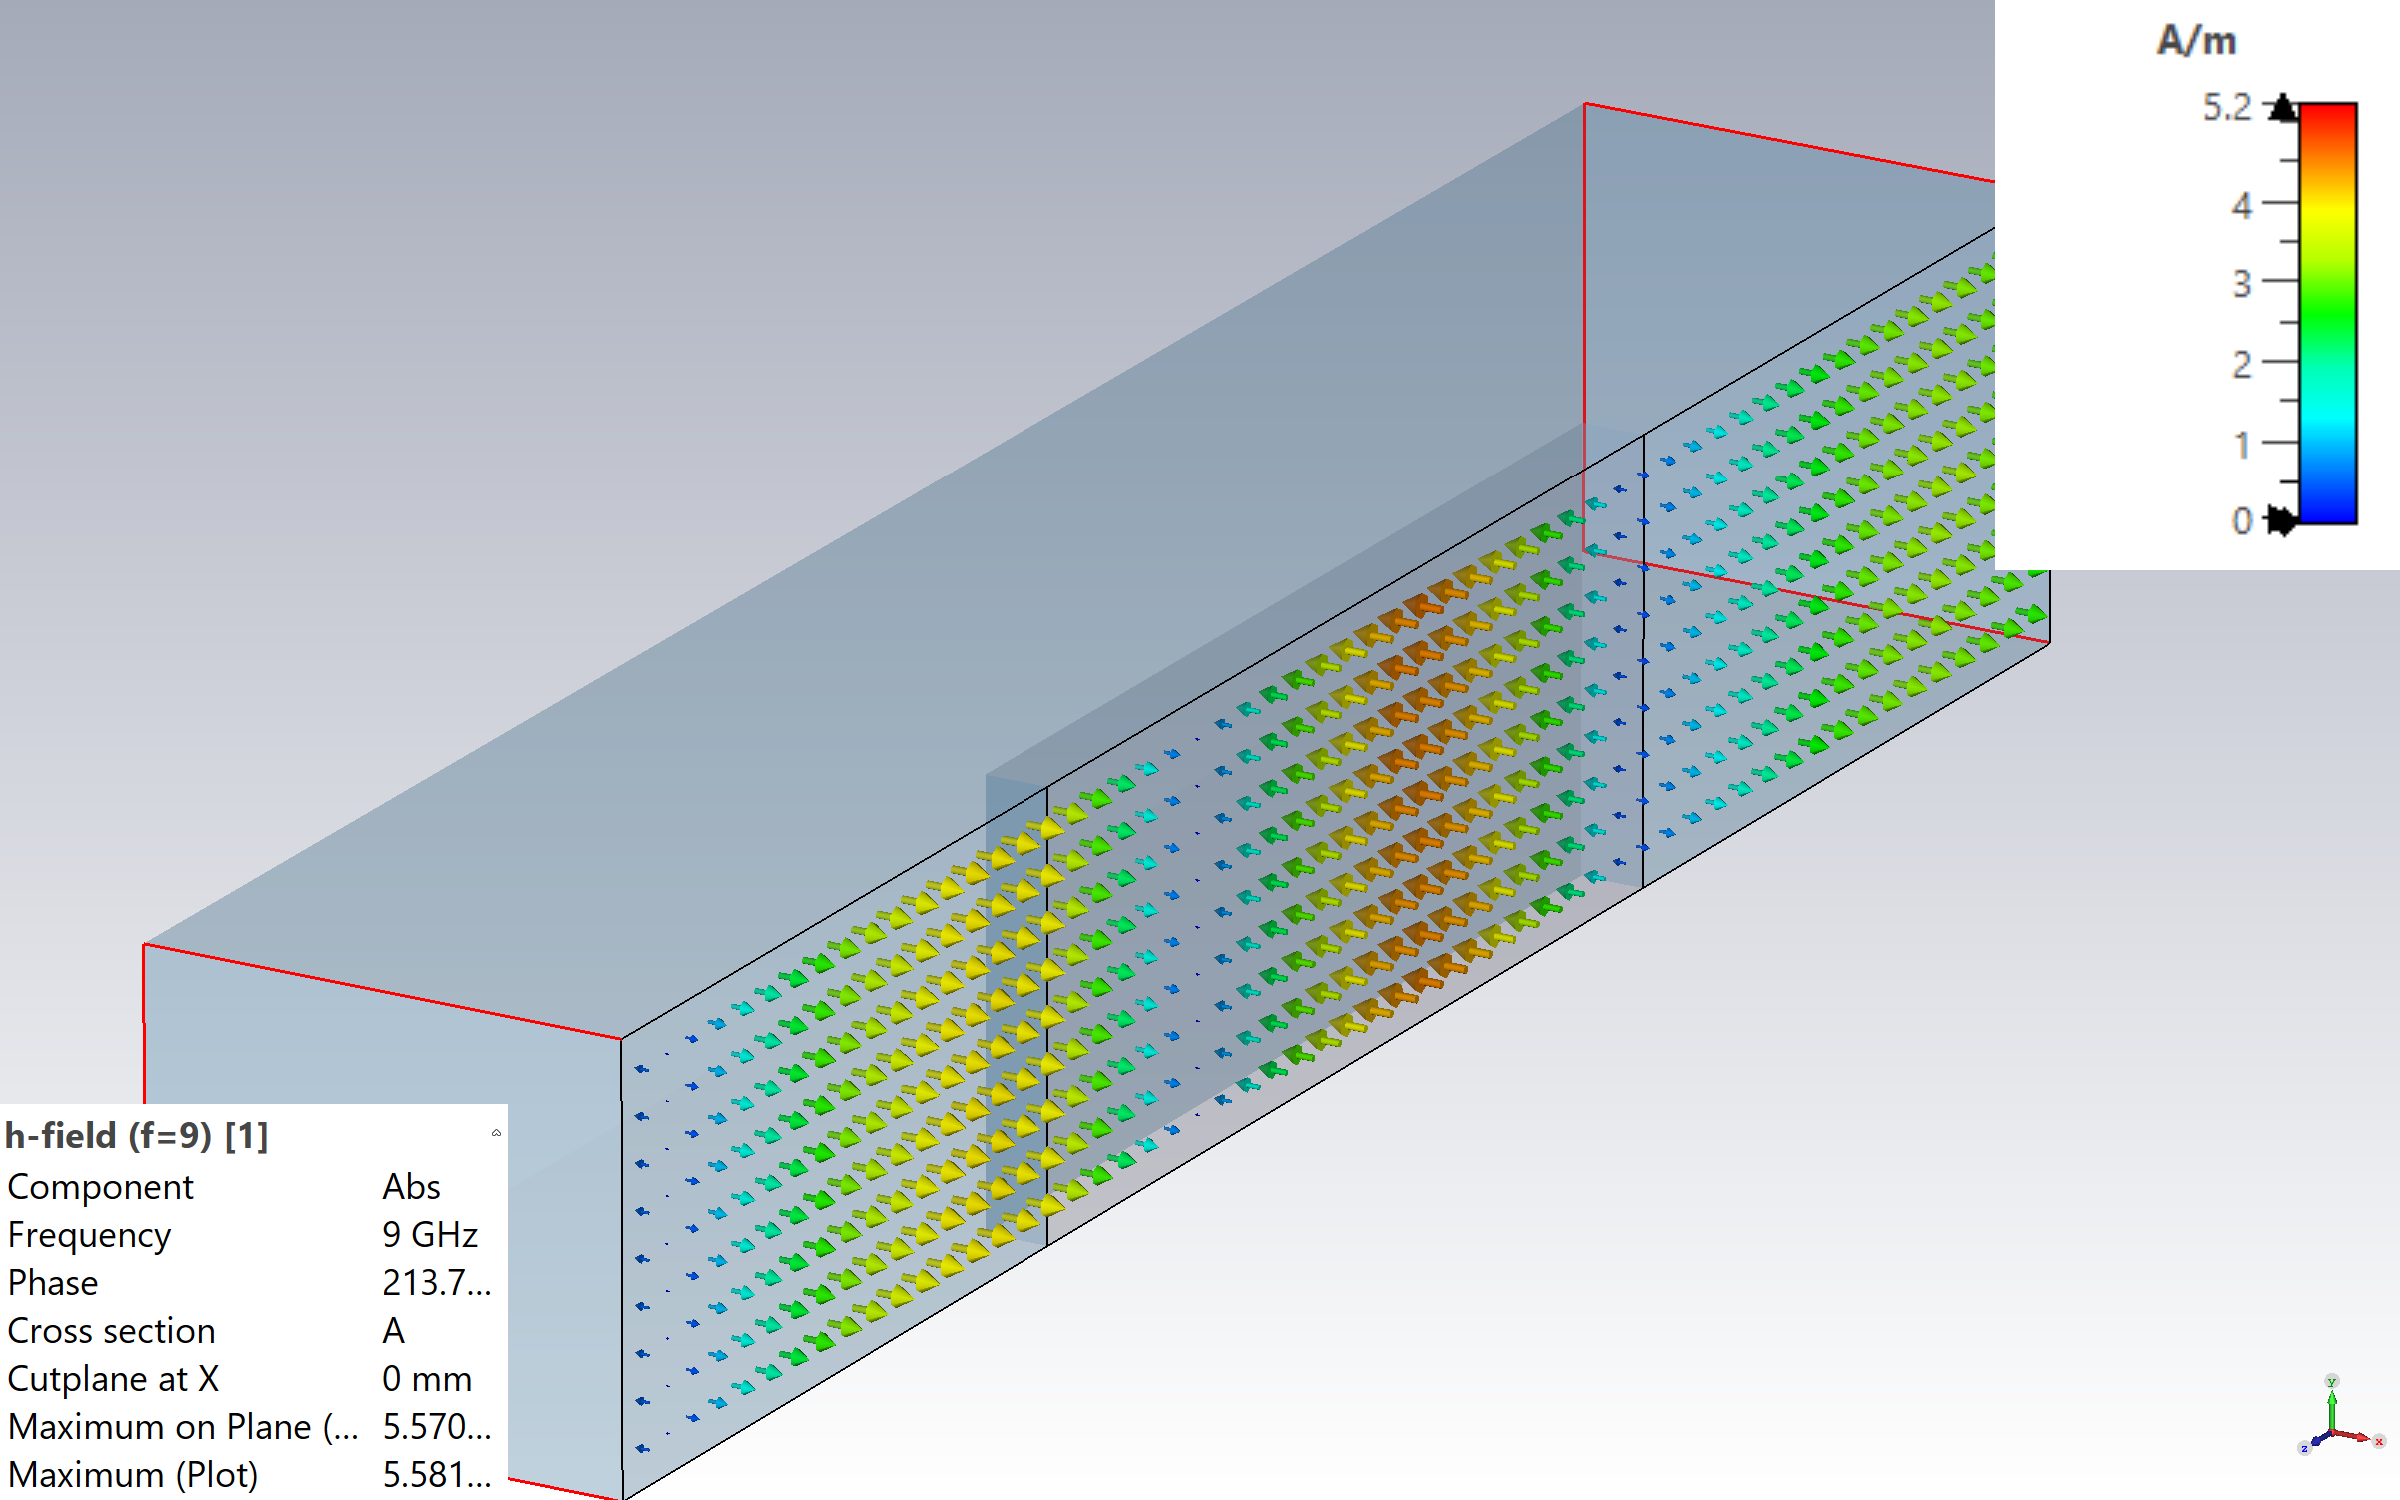
\includegraphics[width=\textwidth]{img/hfield_v2_vector_YZ.png}
        \caption{میدان مغناطیسی --- نمای برداری}
    \end{subfigure}
    \hfill
    \begin{subfigure}[b]{0.48\textwidth}
        \centering
        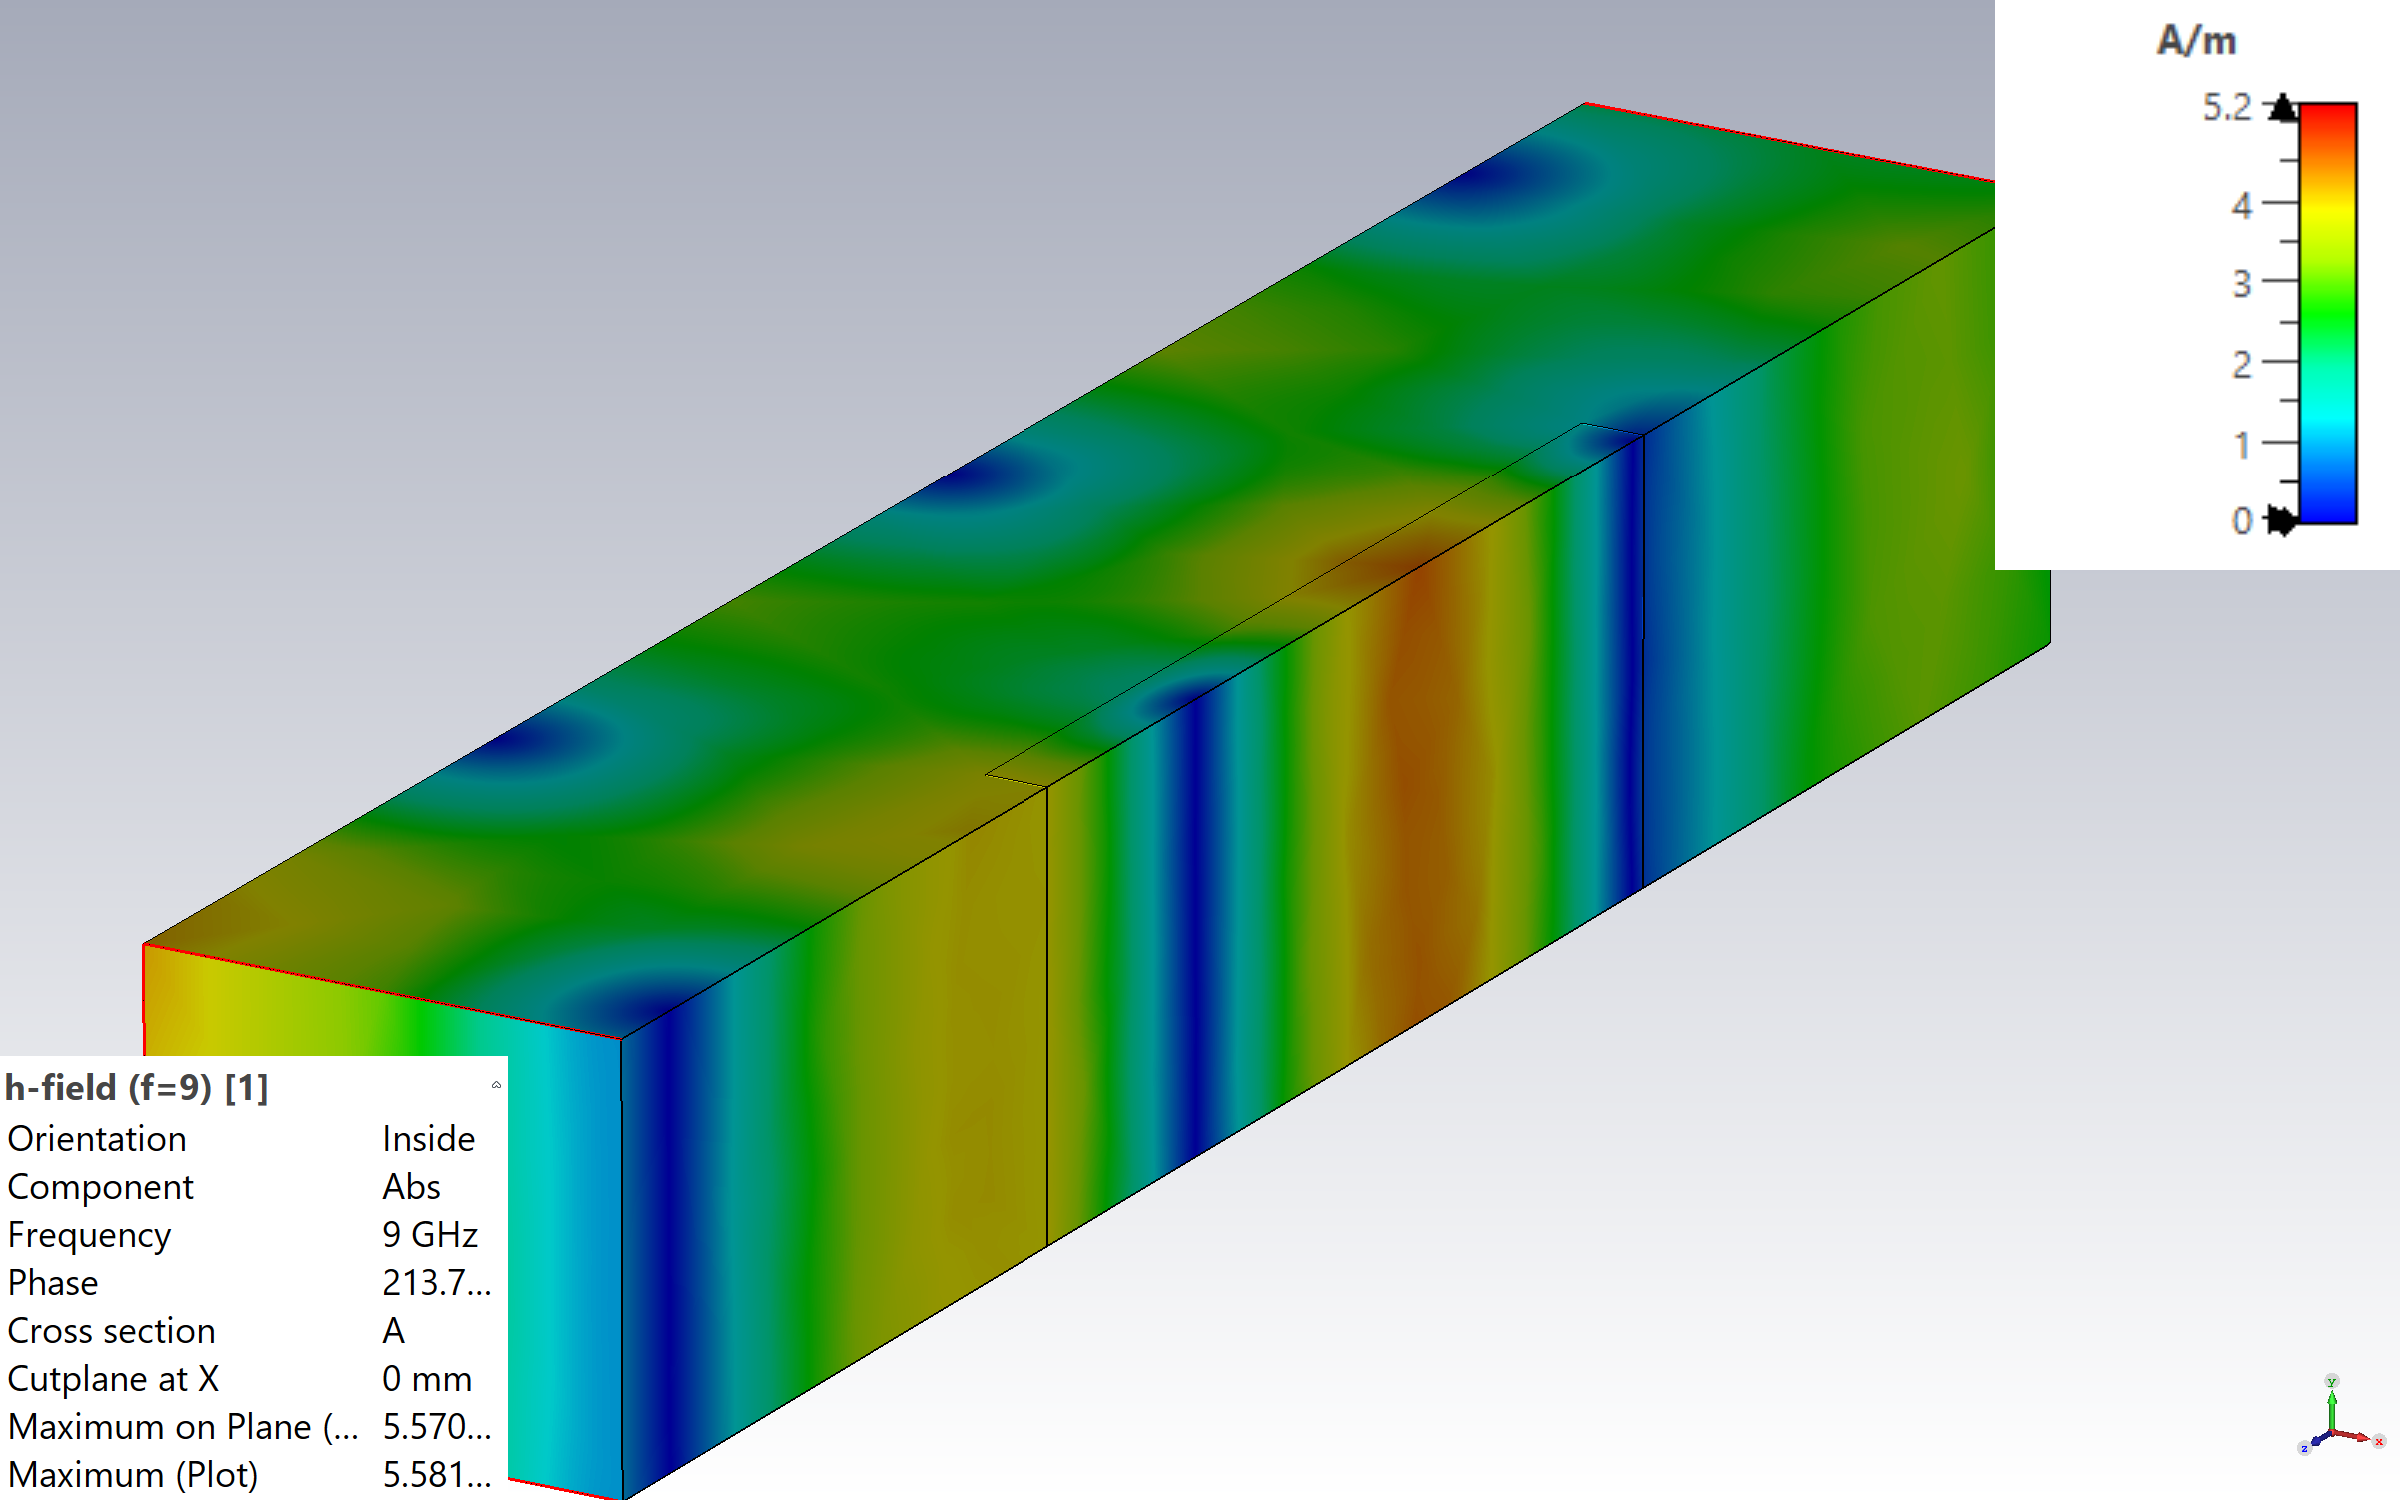
\includegraphics[width=\textwidth]{img/hfield_v2_contour_YZ.png}
        \caption{میدان مغناطیسی --- نمای کانتوری پیوسته}
    \end{subfigure}
    \caption{توزیع میدان مغناطیسی در صفحه طولی عمودی ($YZ$) در $X=0\text{ mm}$ (مقیاس: ۰ تا ۵٫۲ آمپر بر متر).}
    \label{fig:h_yz}
\end{figure}

\section{نتیجه‌گیری و محدودیت‌ها}

\subsection{خلاصه نتایج طراحی و شبیه‌سازی}
در این پروژه، موج‌بر مستطیلی استاندارد \lr{WR-90} بارگذاری‌شده با تیغه تفلون ($\varepsilon_r = 2.1$) در فرکانس مرکزی $9.0\text{ GHz}$ با نرم‌افزار \lr{CST Studio Suite} تحلیل شد:
\begin{enumerate}
    \item \textbf{انطباق فرکانس قطع عددی و تحلیلی:} حل‌کننده پورت موج‌بری CST فرکانس قطع مد غالب $\text{TE}_{10}$ را برابر با $6.557\text{ GHz}$ محاسبه کرده است (\autoref{tab:cst_port}) که با رابطه تحلیلی $f_c = c / (2a) = 6.55706\text{ GHz}$ انطباق صدم درصدی دارد.
    \item \textbf{عملکرد شیفتر فاز:} تیغه دی‌الکتریک با ابعاد $25 \times 10.16 \times 3\text{ mm}$ (طول $\times$ ارتفاع $\times$ ضخامت) شیفت فاز تفاضلی $\Delta\phi = 53.79^\circ$ ایجاد کرد و افت توان عبوری آن ناچیز و برابر با $|S_{21}| = -0.194\text{ dB}$ (انتقال $95.6\%$ توان) بود.
    \item \textbf{پایداری همگرایی مش:} با افزایش $78.5\%$ تعداد المان‌های تتراهدرال، تغییرات پارامترهای پراکندگی کمتر از $0.007\text{ dB}$ بود که استقلال کامل نتایج از مش را تضمین می‌کند.
    \item \textbf{تحلیل بصری میدان‌ها:} نمایش کانتوری پیوسته سطحی به خوبی محبوس شدن چگالی توان درون تیغه دی‌الکتریک و کاهش طول موج هدایت‌شده به $37.7\text{ mm}$ را بدون خطوط تراز مزاحم نشان داد.
\end{enumerate}

\begin{table}[!htbp]
    \centering
    \caption{مشخصات مدهای پورت ورودی استخراج‌شده توسط حل‌گر پورت CST در فرکانس $9.0\text{ GHz}$}
    \vspace{0.2cm}
    \begin{tabular}{|c|c|c|c|c|}
        \hline
        \textbf{شماره پورت / مد} & \textbf{نوع مد} & \textbf{فرکانس قطع عددی CST} & \textbf{فرکانس قطع تحلیلی} & \textbf{امپدانس خط} \\
        \hline
        Port 1 / Mode 1 & $\text{TE}_{10}$ & $6.557\text{ GHz}$ & $6.557\text{ GHz}$ & $549.9\ \Omega$ \\
        \hline
        Port 1 / Mode 2 & $\text{TE}_{20}$ & $13.114\text{ GHz}$ & $13.114\text{ GHz}$ & ناپایدار (زیر قطع) \\
        \hline
    \end{tabular}
    \label{tab:cst_port}
\end{table}

\subsection{محدودیت‌های مدل‌سازی و شرایط عملی}
در شبیه‌سازی حاضر، دیواره‌های هادی موج‌بر به صورت هادی الکتریکی ایده‌آل \lr{(PEC)} مدل‌سازی شده‌اند. در کاربردهای عملی و ساخت آزمایشگاهی:
\begin{itemize}
    \item دیواره‌ها از جنس مس یا برنج با رسانندگی محدود ($\sigma \approx 5.8 \times 10^7\text{ S/m}$) هستند که تلفات اهمی دیواره ایجاد می‌کنند.
    \item زبری سطح \lr{(Surface Roughness)} در فرکانس‌های بالای مایکروویو به دلیل اثر پوستی \lr{(Skin Depth)} افت هدایتی را افزایش می‌دهد.
    \item لبه‌های تیغه تفلون در ساخت بدون پخ \lr{(Tapering)} مدل شدند که باعث تمرکز میدان در گوشه‌ها می‌شود.
\end{itemize}
بنابراین، تلفات عبوری در نمونه واقعی اندکی بیشتر از مقدار $0.19\text{ dB}$ حاصل از شبیه‌سازی خواهد بود.

\end{document}
